% Plantilla para un Trabajo Fin de Grado de la Universidad de Granada,
% adaptada para el Doble Grado en Ingeniería Informática y Matemáticas.
%
%  Autor: Mario Román.
%  Licencia: GNU GPLv2.
%
% Esta plantilla es una adaptación al castellano de la plantilla
% classicthesis de André Miede, que puede obtenerse en:
%  https://ctan.org/tex-archive/macros/latex/contrib/classicthesis?lang=en
% La plantilla original se licencia en GNU GPLv2.
%
% Esta plantilla usa símbolos de la Universidad de Granada sujetos a la normativa
% de identidad visual corporativa, que puede encontrarse en:
% http://secretariageneral.ugr.es/pages/ivc/normativa
%
% La compilación se realiza con las siguientes instrucciones:
%   pdflatex --shell-escape main.tex
%   bibtex main
%   pdflatex --shell-escape main.tex
%   pdflatex --shell-escape main.tex

% Opciones del tipo de documento
\documentclass[oneside,openright,titlepage,numbers=noenddot,openany,headinclude,footinclude=true,
cleardoublepage=empty,abstractoff,BCOR=5mm,paper=a4,fontsize=12pt,main=spanish]{scrreprt}

% Paquetes de latex que se cargan al inicio. Cubren la entrada de
% texto, gráficos, código fuente y símbolos.
\usepackage[utf8]{inputenc}
\usepackage[T1]{fontenc}

\usepackage{subcaption}
\expandafter\def\csname ver@subfig.sty\endcsname{}

\usepackage[table]{xcolor}
\usepackage[final]{pdfpages}
\usepackage{fixltx2e}
\usepackage{graphicx} % Inclusión de imágenes.
\usepackage{graphics}
\usepackage{grffile}  % Distintos formatos para imágenes.
\usepackage{longtable} % Tablas multipágina.
\usepackage{wrapfig} % Coloca texto alrededor de una figura.
\usepackage{rotating}
\usepackage[normalem]{ulem}
\usepackage{acronym}
\usepackage{amsmath}
\usepackage[inline]{enumitem}
\usepackage{tikz}
\usepackage{adjustbox}
\usetikzlibrary{matrix}
\usetikzlibrary{decorations.text}
\usetikzlibrary{mindmap,shadows}
\usepackage{xcolor}
\usepackage{textcomp}
\usepackage{amssymb}
\usepackage[numbers]{natbib}
\usepackage{capt-of}
\usepackage[colorlinks=true]{hyperref}
\usepackage{tikz} % Diagramas conmutativos.
\usepackage{minted} % Código fuente.
\usepackage[T1]{fontenc}
\usepackage{mathtools}
\usepackage{amsmath}
\usepackage{lineno,hyperref}
\usepackage[utf8]{inputenc}
\usepackage[inline]{enumitem}
\usepackage{tabularx}
\usepackage{tabu}
\usepackage{amsmath}
\usepackage{ amssymb }
\usepackage{tikz}
\usetikzlibrary{matrix}
\usetikzlibrary{decorations.text}
\usepackage{mathtools}
\usepackage{amsmath}
\usepackage{comment}
\usepackage{multirow}
\usepackage{longtable}
\usepackage{booktabs}
\usepackage{url}
\usepackage[multiple]{footmisc}
\usepackage{todonotes}
\usepackage{rotfloat}
\usepackage{graphicx}
\usepackage{ amssymb }
%\usepackage{enumerate}
%\usepackage{natbib}

\usepackage{lscape,caption} 
\usepackage{amssymb}
\usepackage{amsmath}
\usepackage{mathtools, cuted}
%\usepackage{graphicx}
\usepackage{url}
\usepackage{algorithm}
\usepackage{algpseudocode}
\usepackage{color}
\usepackage{booktabs}
\usepackage{stmaryrd}
\usepackage{epstopdf}
\usepackage{pdflscape}
\usepackage{stmaryrd}
\usepackage{array}
%\usepackage{tikz}
\usepackage{caption}
\usepackage{hyperref}

\usepackage{grffile} % extends the file name processing of package graphics 
                         % to support a larger range
    \makeatletter % fix for grffile with XeLaTeX
    \def\Gread@@xetex#1{%
      \IfFileExists{"\Gin@base".bb}%
      {\Gread@eps{\Gin@base.bb}}%
      {\Gread@@xetex@aux#1}%
    }
    \makeatother

\usetikzlibrary{matrix,chains,positioning,decorations.pathreplacing,arrows}


\usepackage{dblfloatfix}
\usepackage{flushend}

\setcounter{tocdepth}{1}

\providecommand{\tightlist}{%
  \setlength{\itemsep}{0pt}\setlength{\parskip}{0pt}}
\graphicspath{{./}{inffus/}}

% Plantilla classicthesis
\usepackage[beramono,eulerchapternumbers,linedheaders,parts,a5paper,dottedtoc,
manychapters,pdfspacing]{classicthesis}

% Geometría y espaciado de párrafos.
\setcounter{secnumdepth}{0}
\usepackage{enumitem}
\setitemize{noitemsep,topsep=0pt,parsep=0pt,partopsep=0pt}
\setlist[enumerate]{topsep=0pt,itemsep=-1ex,partopsep=1ex,parsep=1ex}
\usepackage[top=1in, bottom=1.5in, left=1in, right=1in]{geometry}
\setlength\itemsep{0em}
\setlength{\parindent}{0pt}
\usepackage{parskip}

% Profundidad de la tabla de contenidos.
\setcounter{secnumdepth}{3}

% Usa el paquete minted para mostrar trozos de código.
% Pueden seleccionarse el lenguaje apropiado y el estilo del código.
\usepackage{minted}
\usemintedstyle{colorful}
\setminted{fontsize=\small}
\setminted[haskell]{linenos=false,fontsize=\small}
\renewcommand{\theFancyVerbLine}{\sffamily\textcolor[rgb]{0.5,0.5,1.0}{\oldstylenums{\arabic{FancyVerbLine}}}}

% Archivos de configuración.
%------------------------
% Bibliotecas para matemáticas de latex
%------------------------
\usepackage{amsthm}
\usepackage{amsmath}
\usepackage{tikz}
\usepackage{tikz-cd}
\usetikzlibrary{shapes,fit}
\usepackage{bussproofs}
\EnableBpAbbreviations{}
\usepackage{mathtools}
\usepackage{scalerel}
\usepackage{stmaryrd}
\usepackage{ amssymb }
\usepackage{etoolbox}

%------------------------
% Estilos para los teoremas
%------------------------
\theoremstyle{plain}
\newtheorem{theorem}{Teorema}
\newtheorem{proposition}{Proposición}
\newtheorem{lemma}{Lema}
\newtheorem{corollary}{Corolario}
\theoremstyle{definition}
\newtheorem{definition}{Definición}
\newtheorem{proofs}{Demostración}
\theoremstyle{remark}
\newtheorem{remark}{Comentario}
\newtheorem{exampleth}{Ejemplo}

\begingroup\makeatletter\@for\theoremstyle:=definition,remark,plain\do{\expandafter\g@addto@macro\csname th@\theoremstyle\endcsname{\addtolength\thm@preskip\parskip}}\endgroup

%------------------------
% Macros
% ------------------------

% Aquí pueden añadirse abreviaturas para comandos de latex
% frequentemente usados.
\newcommand*\diff{\mathop{}\!\mathrm{d}}  % En macros.tex se almacenan las opciones y comandos para escribir matemáticas.
% ****************************************************************************************************
% classicthesis-config.tex 
% formerly known as loadpackages.sty, classicthesis-ldpkg.sty, and classicthesis-preamble.sty 
% Use it at the beginning of your ClassicThesis.tex, or as a LaTeX Preamble 
% in your ClassicThesis.{tex,lyx} with % ****************************************************************************************************
% classicthesis-config.tex 
% formerly known as loadpackages.sty, classicthesis-ldpkg.sty, and classicthesis-preamble.sty 
% Use it at the beginning of your ClassicThesis.tex, or as a LaTeX Preamble 
% in your ClassicThesis.{tex,lyx} with % ****************************************************************************************************
% classicthesis-config.tex 
% formerly known as loadpackages.sty, classicthesis-ldpkg.sty, and classicthesis-preamble.sty 
% Use it at the beginning of your ClassicThesis.tex, or as a LaTeX Preamble 
% in your ClassicThesis.{tex,lyx} with \input{classicthesis-config}
% ****************************************************************************************************  
% If you like the classicthesis, then I would appreciate a postcard. 
% My address can be found in the file ClassicThesis.pdf. A collection 
% of the postcards I received so far is available online at 
% http://postcards.miede.de
% ****************************************************************************************************


% ****************************************************************************************************
% 0. Set the encoding of your files. UTF-8 is the only sensible encoding nowadays. If you can't read
% äöüßáéçèê∂åëæƒÏ€ then change the encoding setting in your editor, not the line below. If your editor
% does not support utf8 use another editor!
% ****************************************************************************************************
\PassOptionsToPackage{utf8x}{inputenc}
	\usepackage{inputenc}

% ****************************************************************************************************
% 1. Configure classicthesis for your needs here, e.g., remove "drafting" below 
% in order to deactivate the time-stamp on the pages
% ****************************************************************************************************
\PassOptionsToPackage{eulerchapternumbers,listings,drafting,%
		pdfspacing,%floatperchapter,%linedheaders,%
                subfig,beramono,eulermath,parts,dottedtoc}{classicthesis}                                        
% ********************************************************************
% Available options for classicthesis.sty 
% (see ClassicThesis.pdf for more information):
% drafting
% parts nochapters linedheaders
% eulerchapternumbers beramono eulermath pdfspacing minionprospacing
% tocaligned dottedtoc manychapters
% listings floatperchapter subfig
% ********************************************************************

% ****************************************************************************************************
% 2. Personal data and user ad-hoc commands
% ****************************************************************************************************
\newcommand{\myTitle}{A Classic Thesis Style\xspace}
\newcommand{\mySubtitle}{An Homage to The Elements of Typographic Style\xspace}
\newcommand{\myDegree}{Doktor-Ingenieur (Dr.-Ing.)\xspace}
\newcommand{\myName}{André Miede\xspace}
\newcommand{\myProf}{Put name here\xspace}
\newcommand{\myOtherProf}{Put name here\xspace}
\newcommand{\mySupervisor}{Put name here\xspace}
\newcommand{\myFaculty}{Put data here\xspace}
\newcommand{\myDepartment}{Put data here\xspace}
\newcommand{\myUni}{Put data here\xspace}
\newcommand{\myLocation}{Saarbrücken\xspace}
\newcommand{\myTime}{September 2015\xspace}
%\newcommand{\myVersion}{version 4.2\xspace}

% ********************************************************************
% Setup, finetuning, and useful commands
% ********************************************************************
\newcounter{dummy} % necessary for correct hyperlinks (to index, bib, etc.)
\newlength{\abcd} % for ab..z string length calculation
\providecommand{\mLyX}{L\kern-.1667em\lower.25em\hbox{Y}\kern-.125emX\@}
\newcommand{\ie}{i.\,e.}
\newcommand{\Ie}{I.\,e.}
\newcommand{\eg}{e.\,g.}
\newcommand{\Eg}{E.\,g.} 
% ****************************************************************************************************


% ****************************************************************************************************
% 3. Loading some handy packages
% ****************************************************************************************************
% ******************************************************************** 
% Packages with options that might require adjustments
% ******************************************************************** 
%\PassOptionsToPackage{ngerman,american}{babel}   % change this to your language(s)
% Spanish languages need extra options in order to work with this template
% \PassOptionsToPackage{es-lcroman,spanish}{babel}
\usepackage[spanish]{babel}

%\usepackage{csquotes}
% \PassOptionsToPackage{%
%     %backend=biber, %instead of bibtex
% 	backend=bibtex8,bibencoding=ascii,%
% 	language=auto,%
% 	style=alpha,%
%     %style=authoryear-comp, % Author 1999, 2010
%     %bibstyle=authoryear,dashed=false, % dashed: substitute rep. author with ---
%     sorting=nyt, % name, year, title
%     maxbibnames=10, % default: 3, et al.
%     %backref=true,%
%     natbib=true % natbib compatibility mode (\citep and \citet still work)
% }{biblatex}
%     \usepackage{biblatex}

% \PassOptionsToPackage{fleqn}{amsmath}       % math environments and more by the AMS 
%     \usepackage{amsmath}

% ******************************************************************** 
% General useful packages
% ******************************************************************** 
\PassOptionsToPackage{T1}{fontenc} % T2A for cyrillics
    \usepackage{fontenc}     
\usepackage{textcomp} % fix warning with missing font shapes
\usepackage{scrhack} % fix warnings when using KOMA with listings package          
\usepackage{xspace} % to get the spacing after macros right  
\usepackage{mparhack} % get marginpar right
\usepackage{fixltx2e} % fixes some LaTeX stuff --> since 2015 in the LaTeX kernel (see below)
%\usepackage[latest]{latexrelease} % will be used once available in more distributions (ISSUE #107)
\PassOptionsToPackage{printonlyused,smaller}{acronym} 
    \usepackage{acronym} % nice macros for handling all acronyms in the thesis
    %\renewcommand{\bflabel}[1]{{#1}\hfill} % fix the list of acronyms --> no longer working
    %\renewcommand*{\acsfont}[1]{\textsc{#1}} 
    \renewcommand*{\aclabelfont}[1]{\acsfont{#1}}
% ****************************************************************************************************


% ****************************************************************************************************
% 4. Setup floats: tables, (sub)figures, and captions
% ****************************************************************************************************
\usepackage{tabularx} % better tables
    \setlength{\extrarowheight}{3pt} % increase table row height
\newcommand{\tableheadline}[1]{\multicolumn{1}{c}{\spacedlowsmallcaps{#1}}}
\newcommand{\myfloatalign}{\centering} % to be used with each float for alignment
\usepackage{caption}
% Thanks to cgnieder and Claus Lahiri
% http://tex.stackexchange.com/questions/69349/spacedlowsmallcaps-in-caption-label
% [REMOVED DUE TO OTHER PROBLEMS, SEE ISSUE #82]    
%\DeclareCaptionLabelFormat{smallcaps}{\bothIfFirst{#1}{~}\MakeTextLowercase{\textsc{#2}}}
%\captionsetup{font=small,labelformat=smallcaps} % format=hang,
\captionsetup{font=small} % format=hang,
\usepackage{subfig}  
% ****************************************************************************************************


% ****************************************************************************************************
% 5. Setup code listings
% ****************************************************************************************************
% \usepackage{listings} 
% %\lstset{emph={trueIndex,root},emphstyle=\color{BlueViolet}}%\underbar} % for special keywords
% \lstset{language={Haskell},morekeywords={PassOptionsToPackage,selectlanguage},keywordstyle=\color{RoyalBlue},basicstyle=\small\ttfamily,commentstyle=\color{Green}\ttfamily,stringstyle=\rmfamily,numbers=none,numberstyle=\scriptsize,stepnumber=5,numbersep=8pt,showstringspaces=false,breaklines=true,belowcaptionskip=.75\baselineskip} 
% ****************************************************************************************************             


% ****************************************************************************************************
% 6. PDFLaTeX, hyperreferences and citation backreferences
% ****************************************************************************************************
% ********************************************************************
% Using PDFLaTeX
% ********************************************************************
\PassOptionsToPackage{pdftex,hyperfootnotes=false,pdfpagelabels}{hyperref}
    \usepackage{hyperref}  % backref linktocpage pagebackref
\pdfcompresslevel=9
\pdfadjustspacing=1 
\PassOptionsToPackage{pdftex}{graphicx}
    \usepackage{graphicx} 
 

% ********************************************************************
% Hyperreferences
% ********************************************************************
\hypersetup{%
    %draft, % = no hyperlinking at all (useful in b/w printouts)
    colorlinks=true, linktocpage=true, pdfstartpage=3, pdfstartview=FitV,%
    % uncomment the following line if you want to have black links (e.g., for printing)
    %colorlinks=false, linktocpage=false, pdfstartpage=3, pdfstartview=FitV, pdfborder={0 0 0},%
    breaklinks=true, pdfpagemode=UseNone, pageanchor=true, pdfpagemode=UseOutlines,%
    plainpages=false, bookmarksnumbered, bookmarksopen=true, bookmarksopenlevel=1,%
    hypertexnames=true, pdfhighlight=/O,%nesting=true,%frenchlinks,%
    urlcolor=webbrown, linkcolor=RoyalBlue, citecolor=webgreen, %pagecolor=RoyalBlue,%
    %urlcolor=Black, linkcolor=Black, citecolor=Black, %pagecolor=Black,%
    pdftitle={\myTitle},%
    pdfauthor={\textcopyright\ \myName, \myUni, \myFaculty},%
    pdfsubject={},%
    pdfkeywords={},%
    pdfcreator={pdfLaTeX},%
    pdfproducer={LaTeX with hyperref and classicthesis}%
}   

% ********************************************************************
% Setup autoreferences
% ********************************************************************
% There are some issues regarding autorefnames
% http://www.ureader.de/msg/136221647.aspx
% http://www.tex.ac.uk/cgi-bin/texfaq2html?label=latexwords
% you have to redefine the makros for the 
% language you use, e.g., american, ngerman
% (as chosen when loading babel/AtBeginDocument)
% ********************************************************************
\makeatletter
\@ifpackageloaded{babel}%
    {%
       \addto\extrasamerican{%
			\renewcommand*{\figureautorefname}{Figure}%
			\renewcommand*{\tableautorefname}{Table}%
			\renewcommand*{\partautorefname}{Part}%
			\renewcommand*{\chapterautorefname}{Chapter}%
			\renewcommand*{\sectionautorefname}{Section}%
			\renewcommand*{\subsectionautorefname}{Section}%
			\renewcommand*{\subsubsectionautorefname}{Section}%     
                }%
       \addto\extrasngerman{% 
			\renewcommand*{\paragraphautorefname}{Absatz}%
			\renewcommand*{\subparagraphautorefname}{Unterabsatz}%
			\renewcommand*{\footnoteautorefname}{Fu\"snote}%
			\renewcommand*{\FancyVerbLineautorefname}{Zeile}%
			\renewcommand*{\theoremautorefname}{Theorem}%
			\renewcommand*{\appendixautorefname}{Anhang}%
			\renewcommand*{\equationautorefname}{Gleichung}%        
			\renewcommand*{\itemautorefname}{Punkt}%
                }%  
            % Fix to getting autorefs for subfigures right (thanks to Belinda Vogt for changing the definition)
            \providecommand{\subfigureautorefname}{\figureautorefname}%             
    }{\relax}
\makeatother


% ****************************************************************************************************
% 7. Last calls before the bar closes
% ****************************************************************************************************
% ********************************************************************
% Development Stuff
% ********************************************************************
\listfiles
%\PassOptionsToPackage{l2tabu,orthodox,abort}{nag}
%   \usepackage{nag}
%\PassOptionsToPackage{warning, all}{onlyamsmath}
%   \usepackage{onlyamsmath}

% ********************************************************************
% Last, but not least...
% ********************************************************************
\usepackage{classicthesis} 
% ****************************************************************************************************


% ****************************************************************************************************
% 8. Further adjustments (experimental)
% ****************************************************************************************************
% ********************************************************************
% Changing the text area
% ********************************************************************
%\linespread{1.05} % a bit more for Palatino
%\areaset[current]{312pt}{761pt} % 686 (factor 2.2) + 33 head + 42 head \the\footskip
%\setlength{\marginparwidth}{7em}%
%\setlength{\marginparsep}{2em}%

% ********************************************************************
% Using different fonts
% ********************************************************************
%\usepackage[oldstylenums]{kpfonts} % oldstyle notextcomp
%\usepackage[osf]{libertine}
%\usepackage[light,condensed,math]{iwona}
%\renewcommand{\sfdefault}{iwona}
%\usepackage{lmodern} % <-- no osf support :-(
%\usepackage{cfr-lm} % 
%\usepackage[urw-garamond]{mathdesign} <-- no osf support :-(
%\usepackage[default,osfigures]{opensans} % scale=0.95 
%\usepackage[sfdefault]{FiraSans}
% ****************************************************************************************************

% ****************************************************************************************************  
% If you like the classicthesis, then I would appreciate a postcard. 
% My address can be found in the file ClassicThesis.pdf. A collection 
% of the postcards I received so far is available online at 
% http://postcards.miede.de
% ****************************************************************************************************


% ****************************************************************************************************
% 0. Set the encoding of your files. UTF-8 is the only sensible encoding nowadays. If you can't read
% äöüßáéçèê∂åëæƒÏ€ then change the encoding setting in your editor, not the line below. If your editor
% does not support utf8 use another editor!
% ****************************************************************************************************
\PassOptionsToPackage{utf8x}{inputenc}
	\usepackage{inputenc}

% ****************************************************************************************************
% 1. Configure classicthesis for your needs here, e.g., remove "drafting" below 
% in order to deactivate the time-stamp on the pages
% ****************************************************************************************************
\PassOptionsToPackage{eulerchapternumbers,listings,drafting,%
		pdfspacing,%floatperchapter,%linedheaders,%
                subfig,beramono,eulermath,parts,dottedtoc}{classicthesis}                                        
% ********************************************************************
% Available options for classicthesis.sty 
% (see ClassicThesis.pdf for more information):
% drafting
% parts nochapters linedheaders
% eulerchapternumbers beramono eulermath pdfspacing minionprospacing
% tocaligned dottedtoc manychapters
% listings floatperchapter subfig
% ********************************************************************

% ****************************************************************************************************
% 2. Personal data and user ad-hoc commands
% ****************************************************************************************************
\newcommand{\myTitle}{A Classic Thesis Style\xspace}
\newcommand{\mySubtitle}{An Homage to The Elements of Typographic Style\xspace}
\newcommand{\myDegree}{Doktor-Ingenieur (Dr.-Ing.)\xspace}
\newcommand{\myName}{André Miede\xspace}
\newcommand{\myProf}{Put name here\xspace}
\newcommand{\myOtherProf}{Put name here\xspace}
\newcommand{\mySupervisor}{Put name here\xspace}
\newcommand{\myFaculty}{Put data here\xspace}
\newcommand{\myDepartment}{Put data here\xspace}
\newcommand{\myUni}{Put data here\xspace}
\newcommand{\myLocation}{Saarbrücken\xspace}
\newcommand{\myTime}{September 2015\xspace}
%\newcommand{\myVersion}{version 4.2\xspace}

% ********************************************************************
% Setup, finetuning, and useful commands
% ********************************************************************
\newcounter{dummy} % necessary for correct hyperlinks (to index, bib, etc.)
\newlength{\abcd} % for ab..z string length calculation
\providecommand{\mLyX}{L\kern-.1667em\lower.25em\hbox{Y}\kern-.125emX\@}
\newcommand{\ie}{i.\,e.}
\newcommand{\Ie}{I.\,e.}
\newcommand{\eg}{e.\,g.}
\newcommand{\Eg}{E.\,g.} 
% ****************************************************************************************************


% ****************************************************************************************************
% 3. Loading some handy packages
% ****************************************************************************************************
% ******************************************************************** 
% Packages with options that might require adjustments
% ******************************************************************** 
%\PassOptionsToPackage{ngerman,american}{babel}   % change this to your language(s)
% Spanish languages need extra options in order to work with this template
% \PassOptionsToPackage{es-lcroman,spanish}{babel}
\usepackage[spanish]{babel}

%\usepackage{csquotes}
% \PassOptionsToPackage{%
%     %backend=biber, %instead of bibtex
% 	backend=bibtex8,bibencoding=ascii,%
% 	language=auto,%
% 	style=alpha,%
%     %style=authoryear-comp, % Author 1999, 2010
%     %bibstyle=authoryear,dashed=false, % dashed: substitute rep. author with ---
%     sorting=nyt, % name, year, title
%     maxbibnames=10, % default: 3, et al.
%     %backref=true,%
%     natbib=true % natbib compatibility mode (\citep and \citet still work)
% }{biblatex}
%     \usepackage{biblatex}

% \PassOptionsToPackage{fleqn}{amsmath}       % math environments and more by the AMS 
%     \usepackage{amsmath}

% ******************************************************************** 
% General useful packages
% ******************************************************************** 
\PassOptionsToPackage{T1}{fontenc} % T2A for cyrillics
    \usepackage{fontenc}     
\usepackage{textcomp} % fix warning with missing font shapes
\usepackage{scrhack} % fix warnings when using KOMA with listings package          
\usepackage{xspace} % to get the spacing after macros right  
\usepackage{mparhack} % get marginpar right
\usepackage{fixltx2e} % fixes some LaTeX stuff --> since 2015 in the LaTeX kernel (see below)
%\usepackage[latest]{latexrelease} % will be used once available in more distributions (ISSUE #107)
\PassOptionsToPackage{printonlyused,smaller}{acronym} 
    \usepackage{acronym} % nice macros for handling all acronyms in the thesis
    %\renewcommand{\bflabel}[1]{{#1}\hfill} % fix the list of acronyms --> no longer working
    %\renewcommand*{\acsfont}[1]{\textsc{#1}} 
    \renewcommand*{\aclabelfont}[1]{\acsfont{#1}}
% ****************************************************************************************************


% ****************************************************************************************************
% 4. Setup floats: tables, (sub)figures, and captions
% ****************************************************************************************************
\usepackage{tabularx} % better tables
    \setlength{\extrarowheight}{3pt} % increase table row height
\newcommand{\tableheadline}[1]{\multicolumn{1}{c}{\spacedlowsmallcaps{#1}}}
\newcommand{\myfloatalign}{\centering} % to be used with each float for alignment
\usepackage{caption}
% Thanks to cgnieder and Claus Lahiri
% http://tex.stackexchange.com/questions/69349/spacedlowsmallcaps-in-caption-label
% [REMOVED DUE TO OTHER PROBLEMS, SEE ISSUE #82]    
%\DeclareCaptionLabelFormat{smallcaps}{\bothIfFirst{#1}{~}\MakeTextLowercase{\textsc{#2}}}
%\captionsetup{font=small,labelformat=smallcaps} % format=hang,
\captionsetup{font=small} % format=hang,
\usepackage{subfig}  
% ****************************************************************************************************


% ****************************************************************************************************
% 5. Setup code listings
% ****************************************************************************************************
% \usepackage{listings} 
% %\lstset{emph={trueIndex,root},emphstyle=\color{BlueViolet}}%\underbar} % for special keywords
% \lstset{language={Haskell},morekeywords={PassOptionsToPackage,selectlanguage},keywordstyle=\color{RoyalBlue},basicstyle=\small\ttfamily,commentstyle=\color{Green}\ttfamily,stringstyle=\rmfamily,numbers=none,numberstyle=\scriptsize,stepnumber=5,numbersep=8pt,showstringspaces=false,breaklines=true,belowcaptionskip=.75\baselineskip} 
% ****************************************************************************************************             


% ****************************************************************************************************
% 6. PDFLaTeX, hyperreferences and citation backreferences
% ****************************************************************************************************
% ********************************************************************
% Using PDFLaTeX
% ********************************************************************
\PassOptionsToPackage{pdftex,hyperfootnotes=false,pdfpagelabels}{hyperref}
    \usepackage{hyperref}  % backref linktocpage pagebackref
\pdfcompresslevel=9
\pdfadjustspacing=1 
\PassOptionsToPackage{pdftex}{graphicx}
    \usepackage{graphicx} 
 

% ********************************************************************
% Hyperreferences
% ********************************************************************
\hypersetup{%
    %draft, % = no hyperlinking at all (useful in b/w printouts)
    colorlinks=true, linktocpage=true, pdfstartpage=3, pdfstartview=FitV,%
    % uncomment the following line if you want to have black links (e.g., for printing)
    %colorlinks=false, linktocpage=false, pdfstartpage=3, pdfstartview=FitV, pdfborder={0 0 0},%
    breaklinks=true, pdfpagemode=UseNone, pageanchor=true, pdfpagemode=UseOutlines,%
    plainpages=false, bookmarksnumbered, bookmarksopen=true, bookmarksopenlevel=1,%
    hypertexnames=true, pdfhighlight=/O,%nesting=true,%frenchlinks,%
    urlcolor=webbrown, linkcolor=RoyalBlue, citecolor=webgreen, %pagecolor=RoyalBlue,%
    %urlcolor=Black, linkcolor=Black, citecolor=Black, %pagecolor=Black,%
    pdftitle={\myTitle},%
    pdfauthor={\textcopyright\ \myName, \myUni, \myFaculty},%
    pdfsubject={},%
    pdfkeywords={},%
    pdfcreator={pdfLaTeX},%
    pdfproducer={LaTeX with hyperref and classicthesis}%
}   

% ********************************************************************
% Setup autoreferences
% ********************************************************************
% There are some issues regarding autorefnames
% http://www.ureader.de/msg/136221647.aspx
% http://www.tex.ac.uk/cgi-bin/texfaq2html?label=latexwords
% you have to redefine the makros for the 
% language you use, e.g., american, ngerman
% (as chosen when loading babel/AtBeginDocument)
% ********************************************************************
\makeatletter
\@ifpackageloaded{babel}%
    {%
       \addto\extrasamerican{%
			\renewcommand*{\figureautorefname}{Figure}%
			\renewcommand*{\tableautorefname}{Table}%
			\renewcommand*{\partautorefname}{Part}%
			\renewcommand*{\chapterautorefname}{Chapter}%
			\renewcommand*{\sectionautorefname}{Section}%
			\renewcommand*{\subsectionautorefname}{Section}%
			\renewcommand*{\subsubsectionautorefname}{Section}%     
                }%
       \addto\extrasngerman{% 
			\renewcommand*{\paragraphautorefname}{Absatz}%
			\renewcommand*{\subparagraphautorefname}{Unterabsatz}%
			\renewcommand*{\footnoteautorefname}{Fu\"snote}%
			\renewcommand*{\FancyVerbLineautorefname}{Zeile}%
			\renewcommand*{\theoremautorefname}{Theorem}%
			\renewcommand*{\appendixautorefname}{Anhang}%
			\renewcommand*{\equationautorefname}{Gleichung}%        
			\renewcommand*{\itemautorefname}{Punkt}%
                }%  
            % Fix to getting autorefs for subfigures right (thanks to Belinda Vogt for changing the definition)
            \providecommand{\subfigureautorefname}{\figureautorefname}%             
    }{\relax}
\makeatother


% ****************************************************************************************************
% 7. Last calls before the bar closes
% ****************************************************************************************************
% ********************************************************************
% Development Stuff
% ********************************************************************
\listfiles
%\PassOptionsToPackage{l2tabu,orthodox,abort}{nag}
%   \usepackage{nag}
%\PassOptionsToPackage{warning, all}{onlyamsmath}
%   \usepackage{onlyamsmath}

% ********************************************************************
% Last, but not least...
% ********************************************************************
\usepackage{classicthesis} 
% ****************************************************************************************************


% ****************************************************************************************************
% 8. Further adjustments (experimental)
% ****************************************************************************************************
% ********************************************************************
% Changing the text area
% ********************************************************************
%\linespread{1.05} % a bit more for Palatino
%\areaset[current]{312pt}{761pt} % 686 (factor 2.2) + 33 head + 42 head \the\footskip
%\setlength{\marginparwidth}{7em}%
%\setlength{\marginparsep}{2em}%

% ********************************************************************
% Using different fonts
% ********************************************************************
%\usepackage[oldstylenums]{kpfonts} % oldstyle notextcomp
%\usepackage[osf]{libertine}
%\usepackage[light,condensed,math]{iwona}
%\renewcommand{\sfdefault}{iwona}
%\usepackage{lmodern} % <-- no osf support :-(
%\usepackage{cfr-lm} % 
%\usepackage[urw-garamond]{mathdesign} <-- no osf support :-(
%\usepackage[default,osfigures]{opensans} % scale=0.95 
%\usepackage[sfdefault]{FiraSans}
% ****************************************************************************************************

% ****************************************************************************************************  
% If you like the classicthesis, then I would appreciate a postcard. 
% My address can be found in the file ClassicThesis.pdf. A collection 
% of the postcards I received so far is available online at 
% http://postcards.miede.de
% ****************************************************************************************************


% ****************************************************************************************************
% 0. Set the encoding of your files. UTF-8 is the only sensible encoding nowadays. If you can't read
% äöüßáéçèê∂åëæƒÏ€ then change the encoding setting in your editor, not the line below. If your editor
% does not support utf8 use another editor!
% ****************************************************************************************************
\PassOptionsToPackage{utf8x}{inputenc}
	\usepackage{inputenc}

% ****************************************************************************************************
% 1. Configure classicthesis for your needs here, e.g., remove "drafting" below 
% in order to deactivate the time-stamp on the pages
% ****************************************************************************************************
\PassOptionsToPackage{eulerchapternumbers,listings,drafting,%
		pdfspacing,%floatperchapter,%linedheaders,%
                subfig,beramono,eulermath,parts,dottedtoc}{classicthesis}                                        
% ********************************************************************
% Available options for classicthesis.sty 
% (see ClassicThesis.pdf for more information):
% drafting
% parts nochapters linedheaders
% eulerchapternumbers beramono eulermath pdfspacing minionprospacing
% tocaligned dottedtoc manychapters
% listings floatperchapter subfig
% ********************************************************************

% ****************************************************************************************************
% 2. Personal data and user ad-hoc commands
% ****************************************************************************************************
\newcommand{\myTitle}{A Classic Thesis Style\xspace}
\newcommand{\mySubtitle}{An Homage to The Elements of Typographic Style\xspace}
\newcommand{\myDegree}{Doktor-Ingenieur (Dr.-Ing.)\xspace}
\newcommand{\myName}{André Miede\xspace}
\newcommand{\myProf}{Put name here\xspace}
\newcommand{\myOtherProf}{Put name here\xspace}
\newcommand{\mySupervisor}{Put name here\xspace}
\newcommand{\myFaculty}{Put data here\xspace}
\newcommand{\myDepartment}{Put data here\xspace}
\newcommand{\myUni}{Put data here\xspace}
\newcommand{\myLocation}{Saarbrücken\xspace}
\newcommand{\myTime}{September 2015\xspace}
%\newcommand{\myVersion}{version 4.2\xspace}

% ********************************************************************
% Setup, finetuning, and useful commands
% ********************************************************************
\newcounter{dummy} % necessary for correct hyperlinks (to index, bib, etc.)
\newlength{\abcd} % for ab..z string length calculation
\providecommand{\mLyX}{L\kern-.1667em\lower.25em\hbox{Y}\kern-.125emX\@}
\newcommand{\ie}{i.\,e.}
\newcommand{\Ie}{I.\,e.}
\newcommand{\eg}{e.\,g.}
\newcommand{\Eg}{E.\,g.} 
% ****************************************************************************************************


% ****************************************************************************************************
% 3. Loading some handy packages
% ****************************************************************************************************
% ******************************************************************** 
% Packages with options that might require adjustments
% ******************************************************************** 
%\PassOptionsToPackage{ngerman,american}{babel}   % change this to your language(s)
% Spanish languages need extra options in order to work with this template
% \PassOptionsToPackage{es-lcroman,spanish}{babel}
\usepackage[spanish]{babel}

%\usepackage{csquotes}
% \PassOptionsToPackage{%
%     %backend=biber, %instead of bibtex
% 	backend=bibtex8,bibencoding=ascii,%
% 	language=auto,%
% 	style=alpha,%
%     %style=authoryear-comp, % Author 1999, 2010
%     %bibstyle=authoryear,dashed=false, % dashed: substitute rep. author with ---
%     sorting=nyt, % name, year, title
%     maxbibnames=10, % default: 3, et al.
%     %backref=true,%
%     natbib=true % natbib compatibility mode (\citep and \citet still work)
% }{biblatex}
%     \usepackage{biblatex}

% \PassOptionsToPackage{fleqn}{amsmath}       % math environments and more by the AMS 
%     \usepackage{amsmath}

% ******************************************************************** 
% General useful packages
% ******************************************************************** 
\PassOptionsToPackage{T1}{fontenc} % T2A for cyrillics
    \usepackage{fontenc}     
\usepackage{textcomp} % fix warning with missing font shapes
\usepackage{scrhack} % fix warnings when using KOMA with listings package          
\usepackage{xspace} % to get the spacing after macros right  
\usepackage{mparhack} % get marginpar right
\usepackage{fixltx2e} % fixes some LaTeX stuff --> since 2015 in the LaTeX kernel (see below)
%\usepackage[latest]{latexrelease} % will be used once available in more distributions (ISSUE #107)
\PassOptionsToPackage{printonlyused,smaller}{acronym} 
    \usepackage{acronym} % nice macros for handling all acronyms in the thesis
    %\renewcommand{\bflabel}[1]{{#1}\hfill} % fix the list of acronyms --> no longer working
    %\renewcommand*{\acsfont}[1]{\textsc{#1}} 
    \renewcommand*{\aclabelfont}[1]{\acsfont{#1}}
% ****************************************************************************************************


% ****************************************************************************************************
% 4. Setup floats: tables, (sub)figures, and captions
% ****************************************************************************************************
\usepackage{tabularx} % better tables
    \setlength{\extrarowheight}{3pt} % increase table row height
\newcommand{\tableheadline}[1]{\multicolumn{1}{c}{\spacedlowsmallcaps{#1}}}
\newcommand{\myfloatalign}{\centering} % to be used with each float for alignment
\usepackage{caption}
% Thanks to cgnieder and Claus Lahiri
% http://tex.stackexchange.com/questions/69349/spacedlowsmallcaps-in-caption-label
% [REMOVED DUE TO OTHER PROBLEMS, SEE ISSUE #82]    
%\DeclareCaptionLabelFormat{smallcaps}{\bothIfFirst{#1}{~}\MakeTextLowercase{\textsc{#2}}}
%\captionsetup{font=small,labelformat=smallcaps} % format=hang,
\captionsetup{font=small} % format=hang,
\usepackage{subfig}  
% ****************************************************************************************************


% ****************************************************************************************************
% 5. Setup code listings
% ****************************************************************************************************
% \usepackage{listings} 
% %\lstset{emph={trueIndex,root},emphstyle=\color{BlueViolet}}%\underbar} % for special keywords
% \lstset{language={Haskell},morekeywords={PassOptionsToPackage,selectlanguage},keywordstyle=\color{RoyalBlue},basicstyle=\small\ttfamily,commentstyle=\color{Green}\ttfamily,stringstyle=\rmfamily,numbers=none,numberstyle=\scriptsize,stepnumber=5,numbersep=8pt,showstringspaces=false,breaklines=true,belowcaptionskip=.75\baselineskip} 
% ****************************************************************************************************             


% ****************************************************************************************************
% 6. PDFLaTeX, hyperreferences and citation backreferences
% ****************************************************************************************************
% ********************************************************************
% Using PDFLaTeX
% ********************************************************************
\PassOptionsToPackage{pdftex,hyperfootnotes=false,pdfpagelabels}{hyperref}
    \usepackage{hyperref}  % backref linktocpage pagebackref
\pdfcompresslevel=9
\pdfadjustspacing=1 
\PassOptionsToPackage{pdftex}{graphicx}
    \usepackage{graphicx} 
 

% ********************************************************************
% Hyperreferences
% ********************************************************************
\hypersetup{%
    %draft, % = no hyperlinking at all (useful in b/w printouts)
    colorlinks=true, linktocpage=true, pdfstartpage=3, pdfstartview=FitV,%
    % uncomment the following line if you want to have black links (e.g., for printing)
    %colorlinks=false, linktocpage=false, pdfstartpage=3, pdfstartview=FitV, pdfborder={0 0 0},%
    breaklinks=true, pdfpagemode=UseNone, pageanchor=true, pdfpagemode=UseOutlines,%
    plainpages=false, bookmarksnumbered, bookmarksopen=true, bookmarksopenlevel=1,%
    hypertexnames=true, pdfhighlight=/O,%nesting=true,%frenchlinks,%
    urlcolor=webbrown, linkcolor=RoyalBlue, citecolor=webgreen, %pagecolor=RoyalBlue,%
    %urlcolor=Black, linkcolor=Black, citecolor=Black, %pagecolor=Black,%
    pdftitle={\myTitle},%
    pdfauthor={\textcopyright\ \myName, \myUni, \myFaculty},%
    pdfsubject={},%
    pdfkeywords={},%
    pdfcreator={pdfLaTeX},%
    pdfproducer={LaTeX with hyperref and classicthesis}%
}   

% ********************************************************************
% Setup autoreferences
% ********************************************************************
% There are some issues regarding autorefnames
% http://www.ureader.de/msg/136221647.aspx
% http://www.tex.ac.uk/cgi-bin/texfaq2html?label=latexwords
% you have to redefine the makros for the 
% language you use, e.g., american, ngerman
% (as chosen when loading babel/AtBeginDocument)
% ********************************************************************
\makeatletter
\@ifpackageloaded{babel}%
    {%
       \addto\extrasamerican{%
			\renewcommand*{\figureautorefname}{Figure}%
			\renewcommand*{\tableautorefname}{Table}%
			\renewcommand*{\partautorefname}{Part}%
			\renewcommand*{\chapterautorefname}{Chapter}%
			\renewcommand*{\sectionautorefname}{Section}%
			\renewcommand*{\subsectionautorefname}{Section}%
			\renewcommand*{\subsubsectionautorefname}{Section}%     
                }%
       \addto\extrasngerman{% 
			\renewcommand*{\paragraphautorefname}{Absatz}%
			\renewcommand*{\subparagraphautorefname}{Unterabsatz}%
			\renewcommand*{\footnoteautorefname}{Fu\"snote}%
			\renewcommand*{\FancyVerbLineautorefname}{Zeile}%
			\renewcommand*{\theoremautorefname}{Theorem}%
			\renewcommand*{\appendixautorefname}{Anhang}%
			\renewcommand*{\equationautorefname}{Gleichung}%        
			\renewcommand*{\itemautorefname}{Punkt}%
                }%  
            % Fix to getting autorefs for subfigures right (thanks to Belinda Vogt for changing the definition)
            \providecommand{\subfigureautorefname}{\figureautorefname}%             
    }{\relax}
\makeatother


% ****************************************************************************************************
% 7. Last calls before the bar closes
% ****************************************************************************************************
% ********************************************************************
% Development Stuff
% ********************************************************************
\listfiles
%\PassOptionsToPackage{l2tabu,orthodox,abort}{nag}
%   \usepackage{nag}
%\PassOptionsToPackage{warning, all}{onlyamsmath}
%   \usepackage{onlyamsmath}

% ********************************************************************
% Last, but not least...
% ********************************************************************
\usepackage{classicthesis} 
% ****************************************************************************************************


% ****************************************************************************************************
% 8. Further adjustments (experimental)
% ****************************************************************************************************
% ********************************************************************
% Changing the text area
% ********************************************************************
%\linespread{1.05} % a bit more for Palatino
%\areaset[current]{312pt}{761pt} % 686 (factor 2.2) + 33 head + 42 head \the\footskip
%\setlength{\marginparwidth}{7em}%
%\setlength{\marginparsep}{2em}%

% ********************************************************************
% Using different fonts
% ********************************************************************
%\usepackage[oldstylenums]{kpfonts} % oldstyle notextcomp
%\usepackage[osf]{libertine}
%\usepackage[light,condensed,math]{iwona}
%\renewcommand{\sfdefault}{iwona}
%\usepackage{lmodern} % <-- no osf support :-(
%\usepackage{cfr-lm} % 
%\usepackage[urw-garamond]{mathdesign} <-- no osf support :-(
%\usepackage[default,osfigures]{opensans} % scale=0.95 
%\usepackage[sfdefault]{FiraSans}
% ****************************************************************************************************
 % En classicthesis-config.tex se almacenan las opciones propias de la plantilla.

% Color institucional UGR
% \definecolor{ugrColor}{HTML}{ed1c3e} % Versión clara.
\definecolor{ugrColor}{HTML}{c6474b}  % Usado en el título.
\definecolor{ugrColor2}{HTML}{c6474b} % Usado en las secciones.

% Datos de portada
\usepackage{titling} % Facilita los datos de la portada
\author{Mario García Márquez} 
\date{\today}
\title{Mitigando las vulnerabilidades del aprendizaje\\federado mediante Blockchain}

% Portada
\usepackage{datetime}
\usepackage{changepage}
\renewcommand\maketitle{
  \begin{titlepage}
  \changepage{}{}{}{}{}{-.8cm}{}{}{}

    \begin{addmargin}{-1cm}
    \flushright
    \flushleft
    \end{addmargin}
    
    \begin{addmargin}[-2.5cm]{-3cm}
      \begin{center}
        \large  
        \hfill
        \vfill

        \begingroup
        \color{ugrColor}\spacedallcaps{\thetitle} \\ \bigskip
        \endgroup

        \spacedlowsmallcaps{\theauthor}

        \vfill

        Trabajo Fin de Grado \\ \medskip 
        Doble Grado en Ingeniería Informática y Matemáticas \\  \bigskip\bigskip


        \textbf{Tutores}\\
        Nuria Rodríguez Barroso\\ 
        Francisco Herrera Triguero\\ \bigskip

        \spacedlowsmallcaps{Facultad de Ciencias} \\
        \spacedlowsmallcaps{E.T.S. Ingenierías Informática y de Telecomunicación} \\ \medskip
        
        \textit{Granada, \today}

        \vfill                      

      \end{center}  
    \end{addmargin}       
  \end{titlepage}}

\usepackage{wallpaper}
%\usepackage[spanish]{babel}

\DeclareRobustCommand{\chaptertitle}[1]{\textls[80]{\scshape #1}}


\addto\captionsspanish{\renewcommand{\tablename}{Tabla}}

\begin{document}

\ThisULCornerWallPaper{1}{ugrA4.pdf}
\maketitle


\includepdf[pages=-]{pagina_en_blanc.pdf}

\tableofcontents

\thispagestyle{empty}

\newpage


Yo, \textbf{Mario García Márquez}, alumno del \textbf{Doble Grado de Ingeniería Informática y Matemáticas} de la \textbf{Escuela Técnica Superior de Ingeniería Informática y de Telecomunicaciones} y la \textbf{Facultad de Ciencias} de la \textbf{Universidad de Granada}, con DNI 77147974-V, autorizo la ubicación de la siguiente copia de mi Trabajo Fin de Grado en la Biblioteca del Centro para que pueda ser consultada por las personas que lo deseen.



\vspace{25em}

\begin{figure}[H]
\vspace{4em}
    
\includegraphics[scale = 0.6]{firma_mario.jpg}
\end{figure}

Fdo: Mario García Márquez

\begin{flushright}
 Granada a 11 de junio \hspace{0.1em} del 2024
\end{flushright}



\includepdf[pages=-]{pagina_en_blanc.pdf}


\thispagestyle{empty}

D. \textbf{Francisco Herrera Triguero}, Catedrático del Área de Informática del departamento de \textbf{Ciencias de la Computación e Inteligencia Artificial} de la Universidad de Granada, Dª \textbf{Nuria Rodríguez Barroso}, Docente Invitada y Contrado Investigador con Cargo a Proyecto del departamento de \textbf{Ciencias de la Computación e Inteligencia Artificial} de la Universidad de Granada.

\vspace{8em}

Informan:

Que el presente trabajo, titulado \textbf{Mitigando las Vulnerabilidades del Aprendizaje Federado Mediante Blockchain}, ha sido realizado bajo su supervisión por \textbf{Mario García Márquez}, y autorizan la defensa de dicho trabajo ante la Comisión de Evaluación que corresponda.

Y para que conste, expide y firma el presente documento en Granada a 11 de Junio de 2024.


\vspace{10em}

\textbf{Los tutores:}

\begin{minipage}{0.45\textwidth}
\begin{figure}[H]
    
\includegraphics[scale = 0.4]{firma_paco.png}
\end{figure}
\textbf{Francisco Herrera Triguero}
\end{minipage}
\begin{minipage}{0.45\textwidth}
\vspace{2.3cm}

\begin{figure}[H]
    
\includegraphics[scale = 0.75]{firma_nuria.png}
\end{figure}
\textbf{Nuria Rodríguez Barroso}
\end{minipage}



\vspace{10em}



\includepdf[pages=-]{pagina_en_blanc.pdf}

Yo, \textbf{Mario García Márquez}, alumno del \textbf{Doble Grado en Ingeniería Informática y Matemáticas} de la \textbf{Escuela Técnica Superior de Ingeniería Informática y Matemática} y de la \textbf{Facultad de Ciencias} de la \textbf{Universidad de Granada}, con DNI 77147974-V, \underline{declaro explícitamente} que el trabajo presentado es original, entendido en el sentido de que no he utilizado ninguna fuente sin citarla debidamente.

\vspace{25em}

\begin{figure}[H]
\hspace{4em}
    
\includegraphics[scale = 0.6]{firma_mario.jpg}
\end{figure}

Fdo: Mario García Márquez

\begin{flushright}
 Granada a 11 de junio \hspace{0.1em} del  2024
\end{flushright}


\includepdf[pages=-]{pagina_en_blanc.pdf}

\chapter*{Agradecimientos}
\begin{flushleft}
Este trabajo se puede ver como la conclusión de muchos años de educación y aprendizaje. La realización de este no podría haberse llevado a cabo sin la ayuda de mucha gente. Si buscamos al culpable más directo de estar leyendo esto no puedo decir otra persona que no sea mi tutora, Nuria. Durante estos 5 años de carrera me ha acompañado durante casi la mitad de ellos y además de una más que sobresaliente labor docente (porque hay profesores que marcan y eso es algo que se aprende con la experiencia) también es una de las mejores personas que he conocido jamás y una excelente amiga. Muchas gracias por ser el gigante que me ha puesto sobre sus hombros y me ha enseñado el camino a seguir.

Pero quedarnos en el culpable directo sería poco, y es que hay gente que siempre ha estado ahí, como mi familia que siempre me ha servido un apoyo incondicional a cualquier decisión que he tomado y siempre me ha animado con todo lo académico que me ha acabado llenando tanto. También tengo que agradecer a mis compañeros de carrera: Nerea, Javi, Pablo, Maxim, Isa, Inma, Julio, Jaime y muchos más que no cabrían en tan poco espacio. Gracias por hacerme pensar, mejorar y reírme tanto. Aunque las horas de clases se me hayan hecho eternas, habéis logrado que los años se me hayan hecho cortos.

También, pero no menos importante, tengo que agradecer a todos mis compañeros de Alemania que me han dado su calor incluso por los kilómetros que nos separan. Gracias Alba, Fueyo, Dani, Víctor y Ali. Sin vosotros difícilmente sería quien soy ahora y tampoco lo sería así este trabajo.

Muchas gracias a todos.
\end{flushleft}




\includepdf[pages=-]{pagina_en_blanc.pdf}

\chapter*{Resumen}

En este proyecto se estudia el estado actual de la aplicabilidad de las tecnologías de tipo \textit{blockchain} al Aprendizaje Federado (FL) para la mitigación de ataques adversarios. Para ello se implementan arquitecturas estándar de FL y de \textit{blockchain} aplicado a FL, comprobándose su capacidad como defensa ante ataques y se propone una nueva arquitectura que mejora las anteriores en este sentido.

Para introducir el proyecto y conocer mejor sus fundamentos, se realiza una introducción al álgebra lineal, teoría de la probabilidad, inferencia y teoría de la información. De forma seguida, se explica la base de la optimización de funciones no lineales, el operador de agregación Krum y nociones sobre Aprendizaje Automático, más concretamente Aprendizaje Profundo.

Los siguientes capítulos se enfocan en explicar FL, así como los distintos ataques a los que es vulnerable este esquema, haciendo un especial énfasis en los tratados en el trabajo. También se explica la tecnología \textit{blockchain} y sus beneficios en sistemas distribuidos.

Finalmente, se explica el estado actual del paradigma de \textit{blockchain} aplicado a FL, se expone la hipótesis de cómo ciertas arquitecturas podrían servir como una capa de defensa para FL y se propone una nueva arquitectura enfocada en la seguridad del modelo. Esta nueva arquitectura, Krum Federated Chain (KFC), se basa en las propuestas actuales de aplicabilidad de \textit{blockchain} a FL con un efoque especial en defensa logrado por la aplicación del operador de agregación Krum. Esto es seguido por la realización y análisis de una serie de experimentos para contrastar la hipótesis planteada y la propuesta, observando como KFC mejora los métodos de defensa ofrecidos por \textit{blockchain} mantiendo el modelo seguro bajo escenarios más restrictivos, junto a conclusiones y vías de trabajo futuro.


\textbf{Palabras clave}: aprendizaje federado, ataques adversarios, redes neuronales, blockchain, clasificación de imágenes, aprendizaje automático, optimización no lineal.

\includepdf[pages=-]{pagina_en_blanc.pdf}
\chapter*{Abstract}
This study aims to examine the integration of blockchain technologies with Federated Learning (FL), emphasizing the potential of this combination to protect federated frameworks from adversarial attacks. Initially, the context of the problem is introduced.

\section*{Trustworthy AI}
Artificial Intelligence (AI) systems have become an integral part of daily life, often operating unobtrusively. From recommendation systems to Instagram filters, AI significantly influences various aspects of human existence. Recently, the rising prominence of systems such as ChatGPT and autonomous vehicles has sparked widespread concern regarding their security and potential negative impacts on sectors such as healthcare, education, culture, and democracy. In response to these concerns, the concept of Trustworthy AI systems has emerged, founded on several technical requirements.

\section*{Federated Learning}
A critical technical requirement for Trustworthy AI is security and data governance, which has led to the development of Federated Learning (FL). FL is an innovative architecture that enables collaborative model training across decentralized devices while maintaining data privacy. Despite its advantages, the decentralized nature of FL can be a vulnerability. Since data remains in the nodes, traditional data exploration techniques cannot be employed, rendering the framework susceptible to data poisoning attacks.

\section*{Blockchain Applied to Federated Learning}
Blockchain technologies have gained substantial popularity in recent years, partly due to the success of innovations like Bitcoin. The integration of blockchain into FL has emerged as a promising solution to enhance its security and integrity. By leveraging the immutable and transparent nature of blockchain, FL systems can establish a tamper-resistant record of model updates and participant contributions, thereby mitigating the risks of data manipulation and unauthorized access.

\section*{Mathematical Foundation}
To fully comprehend blockchain technology and machine learning, it is essential to delve into the key mathematical concepts underlying these topics.

This foundational chapter begins with an introduction to basic linear algebra, which is a critical component for understanding machine learning models. Subsequently, we explore probability, inference, and information theory. Here, we introduce the fundamental concepts of probability theory, including random variables, probability distributions, and conditional probability. The discussion then progresses to parameter estimation and maximum likelihood estimation, as machine learning models are frequently optimized using these estimators.

Further, the chapter addresses nonlinear optimization, outlining the essential conditions of this theory and explaining the gradient descent method for unconstrained optimization, which is fundamental for optimizing machine learning models. Lastly, we examine the Krum aggregation operator, which provides a robust algorithm for aggregating gradient estimates, ensuring resilience against outliers.

In addition, we address general deep learning algorithms by introducing neural networks from a theoretical perspective. We define the general structure of a neural network, followed by a discussion on the loss function based on cross-entropy. We then define output units and present specific examples such as sigmoidal units. This is followed by an introduction to hidden units, in a manner similar to our treatment of output units.

After establishing a background in general neural networks, we focus on convolutional neural networks (CNNs) and the classification problem. We define the convolution operation, which plays a crucial role in CNN architecture. Finally, we introduce the notion of the EfficientNet architecture, which will be employed during the experiments in this study.

\section*{Blockchain and Federated Learning}
The following chapters provide a formal exposition of FL. We begin by defining an FL system and presenting a taxonomy of the various types of attacks to which FL is vulnerable. We delve deeper into attacks that specifically target the federated model, as well as some current defenses against these attacks that have been explored in the literature.

Next, we explain blockchain systems, detailing their main components and how they can be utilized to preserve trust and privacy throughout the entire system. We then elucidate the consensus mechanisms that enable blockchain systems to make decisions while maintaining a decentralized structure.

Finally, we explore the combination of FL and blockchain, illustrating the current state of this paradigm. We discuss successful applications of this technological integration and examine the different consensus mechanisms and architectures that have been proposed to achieve the proper integration of both technologies.

\section*{Krum Federated Chain}
Having established the core concepts, the subsequent chapters are dedicated to our proposed framework. We begin by hypothesizing that Proof Of Federated Learning (PoFL), a consensus mechanism specifically designed for FL, can, under certain circumstances, serve as a valid defense against adversarial attacks, even though this was not its original purpose.

Inspired by its disadvantages, we then propose Krum Federated Chain (KFC), a novel blockchain architecture applied to FL. This architecture leverages the PoFL consensus mechanism and the Krum aggregation operator to address more complex scenarios where our initial hypothesis does not hold.

Following this, we detail the experimental setup in which multiple image classification models are trained using KFC, along with some standard architectures from the literature, to validate our proposal. We analyze the results, demonstrating how KFC provides a robust defense against adversarial attacks in federated frameworks, even in cases where PoFL alone does not suffice, thereby establishing KFC as a viable architecture for integrating blockchain and FL.

Finally, we present the conclusions of this study and propose potential directions for future research.

\textbf{Keywords}: federated learning, neuronal networks, adversarial attacks, blockchain, image classification, machine learning, non linear optimization.


\includepdf[pages=-]{pagina_en_blanc.pdf}

\chapter*{Lista de abreviaciones}
%\thispagestyle{fancy}

\begin{acronym}[ME-MOEA/D  ]
    \acro{AA}{Aprendizaje Automático}
    \acro{BFT}{Tolerante a Fallos Bizantinos (\textit{Byzantine Fault Tolerance})}
    \acro{CNN}{Red Neuronal Convolucional (Convolutional Neural Network)}
    \acro{DP}{Privacidad Diferencial (\textit{Differential Privacy})}
    \acro{f.d.p.}{Función de Densidad de Probabilidad}
    \acro{FedAvg}{\textit{Federated Averaging}}
    \acro{FL}{Aprendizaje Federado \textit{(Federated Learning)}}
    \acro{f.m.p.}{Función Masa de Probabilidad}
    \acro{FTL}{\textit{Federated Transfer Learning}}
    \acro{HFL}{Aprendizaje Federado Horizontal (\textit{Horizontal Federated Learning})}
    \acro{IA}{Inteligencia Artificial}
    \acro{i.i.d.}{Independientes e Idénticamente Distribuidas}
    \acro{IoT}{Internet de las Cosas}
    \acro{KFC}{\textit{Krum Federated Chain}}
    \acro{lr}{\textit{Learning Rate}}
    \acro{MLP}{Perceptrón Multicapa (\textit{Multilayer Perceptron})}
    \acro{P2P}{\textit{Peer-to-Peer}}
    \acro{PoFL}{Prueba de Aprendizaje Federado (\textit{Proof of Federated Learning})}
    \acro{PoS}{Prueba de Participación (\textit{Proof of Stake})}
    \acro{PoW}{Prueba de Trabajo (\textit{Proof of Work})}
    \acro{v.a.}{Variable Aleatoria}
    \acro{VFL}{Aprendizaje Federado Vertical (\textit{Vertical Federated Learning})}
\end{acronym} % Acronimos


\includepdf[pages=-]{pagina_en_blanc.pdf}

\part{Introducción}

\chapter{Introducción}
% Te escribo aquí el hilo conductor que tienes que seguir, con la filosofía siempre de "una idea, un párrafo":

\section{Contexto}

%1- La IA lleva muchos años en nuestras vidas: ejemplos medio antiguos.
La \ac{IA} ha tenido un impacto significativo en nuestro día a día, aunque a menudo de manera imperceptible. Desde la personalización de recomendaciones de productos en línea hasta encontrar el trayecto óptimo para moverte de un punto a otro en aplicaciones de mapas, la \ac{IA} lleva más de 20 años estando presente en varios aspectos de nuestra vida cotidiana.

%2- Pero últimamente está entrando de lleno y a nuestro día a día: chatGPT, etc. 
Sin embargo, ahora está más presente que nunca. Con la aparición de productos como chatGPT, asistentes de voz como Alexa o Siri, sistemas de reconocimiento facial como FaceID o la conducción autónoma como Tesla Autopilot, la \ac{IA} se ha convertido que una parte fundamental de la vida de muchas personas. También ha aumentado enormemente el interés general, tanto de personas particulares como de empresas, por esta tecnología con el fin de aplicarla a todas las áreas posibles maximizando el beneficio producido por su uso.


% 3- Esto puede ser muy bueno, pero muy ¡PELIGROSO! Hay ciertos contextos (educación, salud, democracia, cultura) donde hay que tener cuidado (high risk AI scenarios según EU Act). 
Aunque aún se está explorando el potencial de la \ac{IA} en varios campos, hay una creciente preocupación sobre cómo sistemas de \ac{IA} no supervisados por humanos pueden causar un impacto negativo en áreas más delicadas como la educación, salud, democracia, justicia, cultura o ciencia. Esto ha llevado a la definición de \textit{High-Risk AI Systems} por parte de \textit{EU AI Act}~\cite{euact}, los cuales son sistemas que pueden suponer un riesgo a los derechos fundamentales de las personas o a su integridad, como sistemas que procesen datos biométricos o aquellos usados en vehículos.

% 4- En este contexto surge Safe AI, trustworhy AI con los siguientes principios (coger el dibujo que usé en mi tesis, puedes citarlo tal cual la fuente).
En este contexto, emergen los conceptos de sistemas de \textit{Trustworthy AI} o \ac{IA} confiable y \textit{Responsible AI}~\cite{trusworth}. Los sistemas de \textit{Trustworthy AI} están basados en siete requisitos técnicos que se deben de mantener durante durante todo el ciclo de vida del sistema de \ac{IA}: 
\begin{enumerate}
    \item Supervisión e inspección humana.
    \item Robustez y seguridad.
    \item Privacidad y gobernanza de los datos.
    \item Transparencia.
    \item Diversidad, no discriminación y equidad.
    \item Bienestar social y ambiental.
    \item Rendición de cuentas.
\end{enumerate}

Estos requisitos están basados en tres pilares fundamentales: (1) legalidad, (2) ética, y (3) robustez, tanto desde perspectivas técnicas como sociales. Estos requisitos y sus pilares quedan ilustrados en la Figura~\ref{fig:tai}.
\begin{figure}
    \centering
    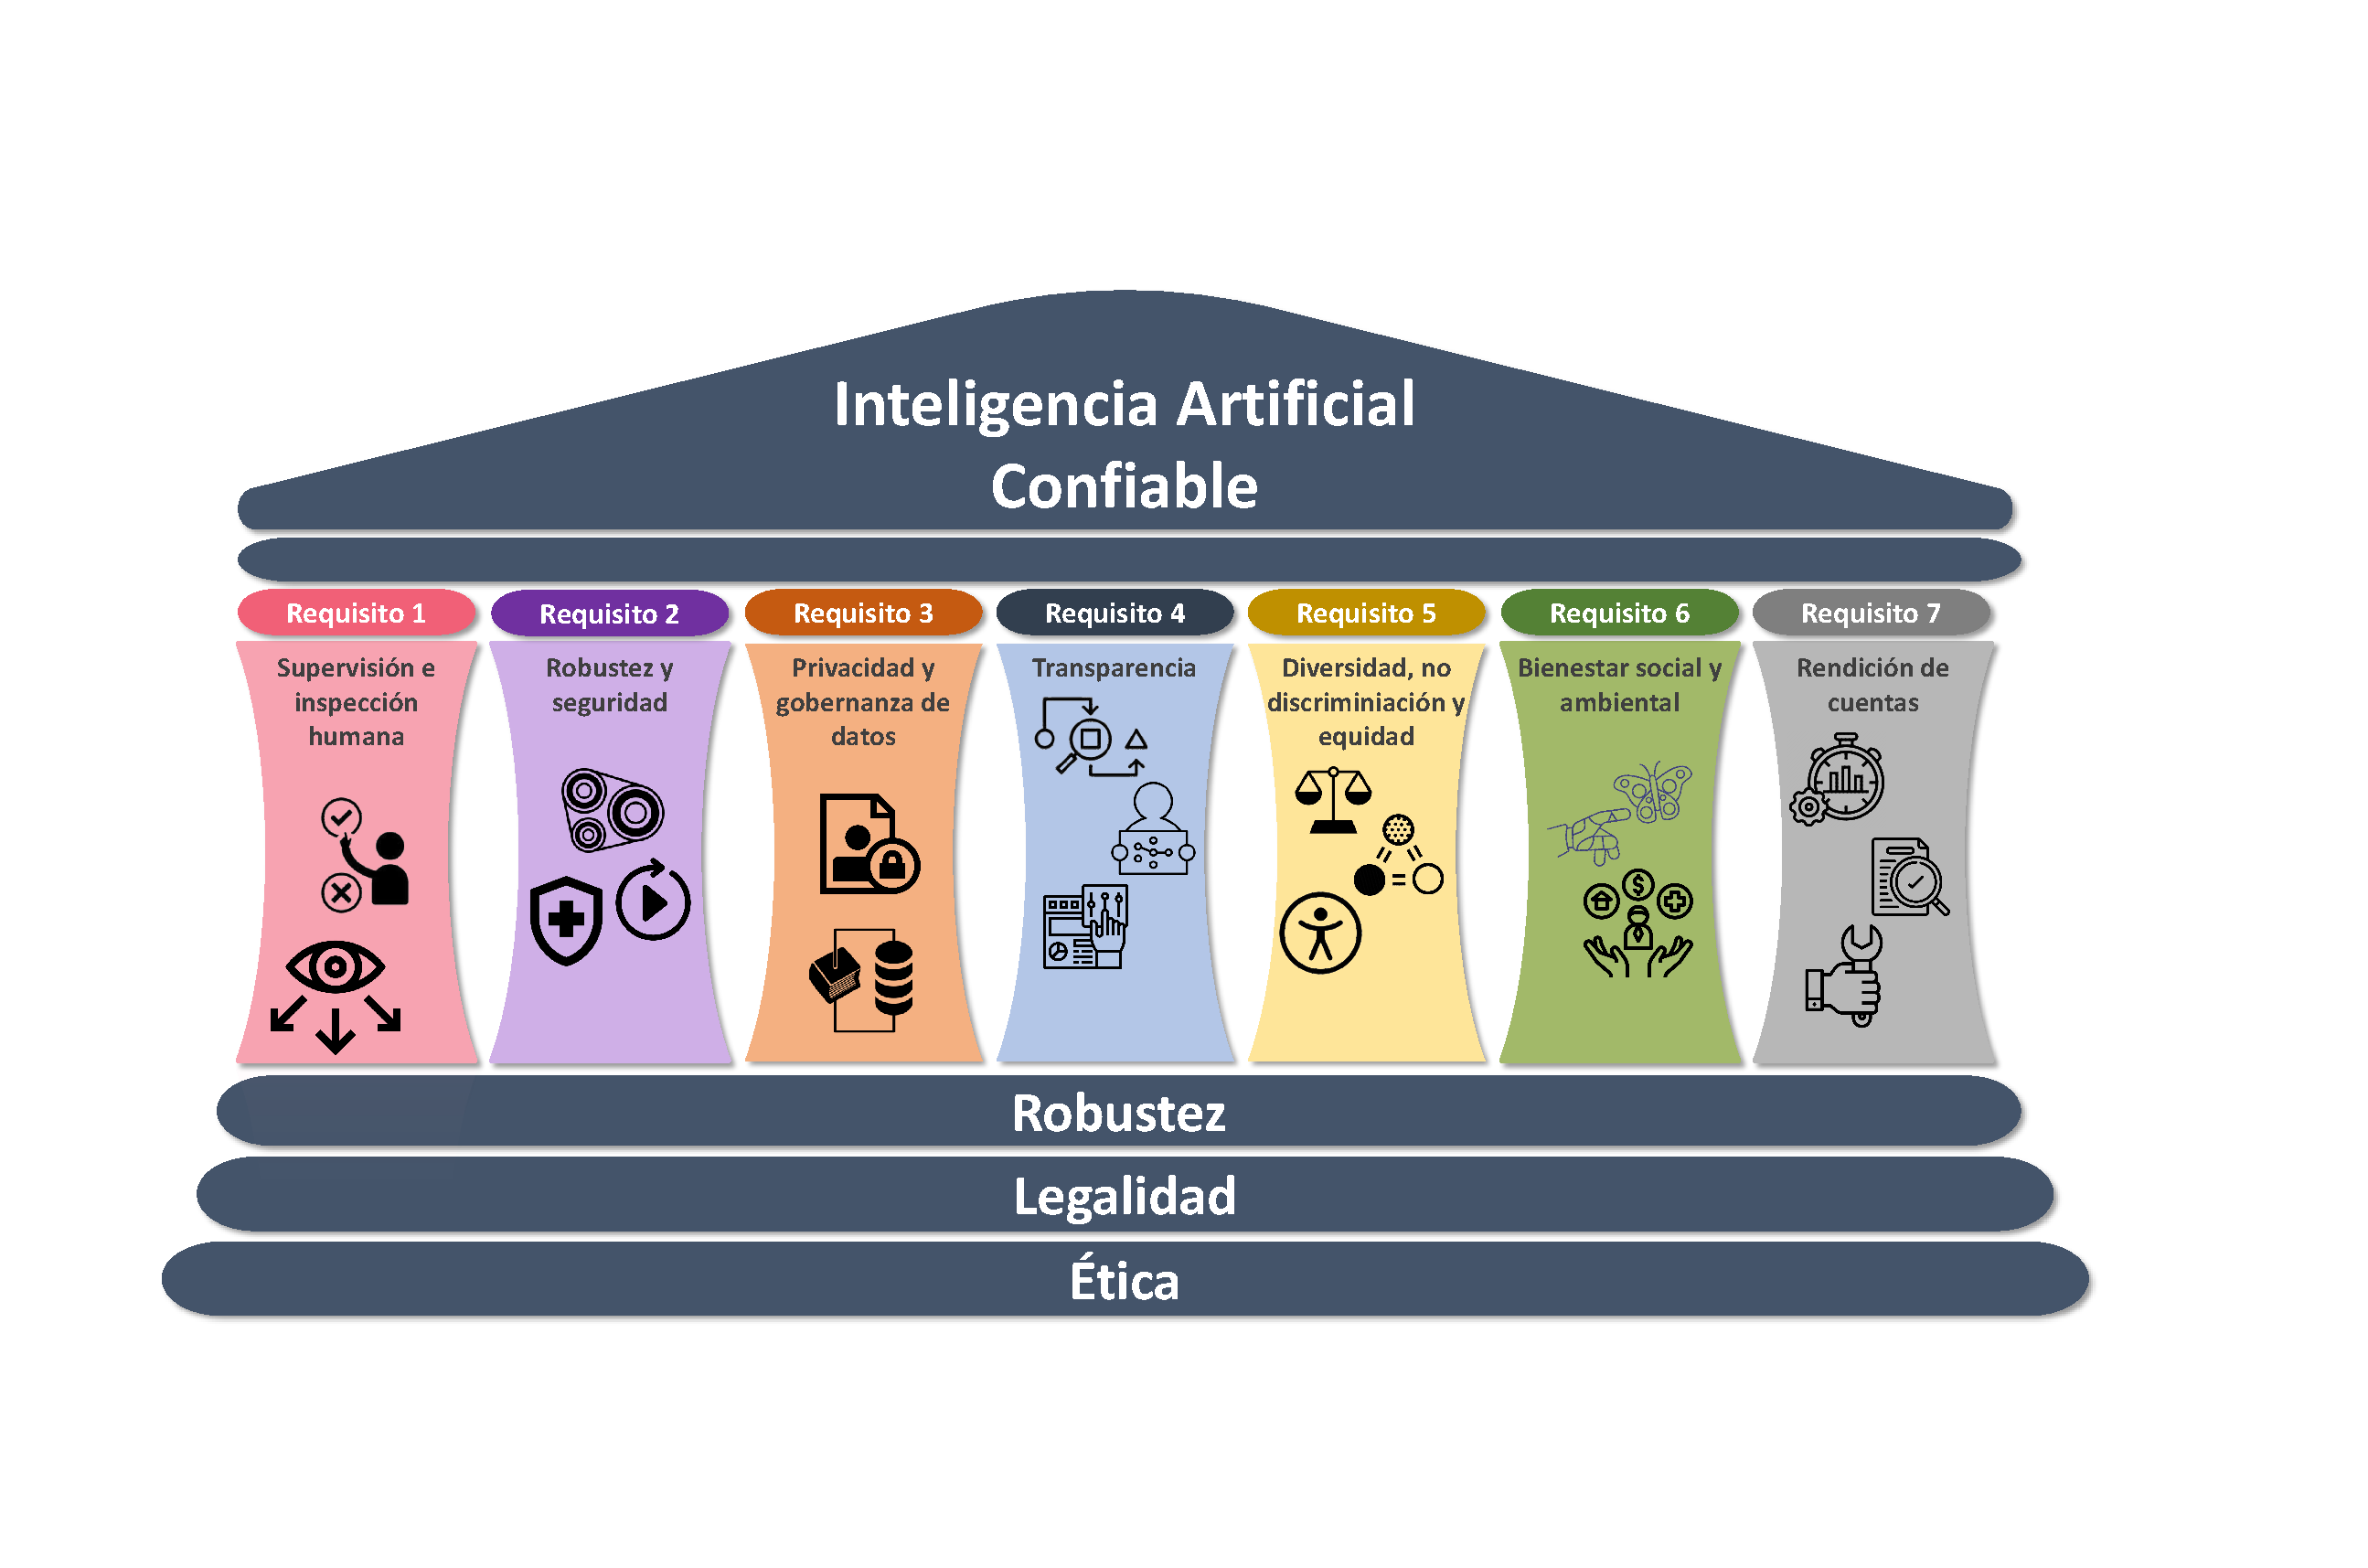
\includegraphics[width=\textwidth]{figuras/TAI.pdf}
    \caption{Diagrama de los requisitos técnicos de un sistema de \textit{Trusworthy AI}. Fuente:~\cite{diaz-tai}.}
    \label{fig:tai}
\end{figure}

% 5- Uno de los principales pialres para asegurar una IA segura y confiable: es la privacidad. En este contexto surge tanto el FL como la blockchain.
Uno de los requisitos técnicos de estos sistemas es garantizar la privacidad. Para ello, en 2016 e impulsado por Google, aparece el concepto de \ac{FL}~\cite{mcmahan-2023}, un paradigma de aprendizaje que permite el entrenamiento distribuido asegurando la privacidad de los datos. También durante este tiempo se aumenta el interés de las masas en las tecnologías \textit{blockchain}, tecnologías que permiten el registro digital descentralizado de transacciones compartidas entre una red que es inmutable, en parte impulsadas por el éxito de Bitcoin~\cite{bitcoin}.

\section{Motivación}

% 6- Parrafito super divulgativo de lo que es el FL y cómo ayuda.
Por su parte, el \ac{FL} permite el entrenamiento de un modelo distribuido sin que los clientes tengan que compartir sus datos privados con ninguna entidad. Para ello cada cliente entrena de manera local un modelo con sus datos personales, siendo este modelo el que luego es compartido con un servidor central, que finalmente agrega todos los resultados de los clientes para obtener un nuevo modelo global. \ac{FL} también incluye más ventajas como costes reducidos en comunicación o robustez respecto a otras alternativas distribuidas.

% 7- Parrafito super divulgativo de lo que es la blockchain y cómo ayuda.
Por otro lado, las tecnologías \textit{blockchain} ofrecen un esquema distribuido para computación~\cite{duc-2023} donde los datos son verificables e inmutables por todas las entidades mediante el uso de funciones criptográficas. A esto hay que añadir que es un sistema descentralizado donde no hay un servidor central, por lo que no hay un único servidor que sea vulnerable a ataques. Otros beneficios de estas tecnologías es una alta escalabilidad y facilidad para rastrear cambios a los datos compartidos~\cite{survey-blockchain}.

% 8- PERO, el FL es vulenrable a ataques adversarios ohhhhhhhhhhhh :(  Y aunque se ha intentado solucionar de muchísimas maneras, no se ha conseguido cubrir esta vulnerabilidad al 100\%.
Debido a estas características, el \ac{FL} se ha empleado en muchas situaciones con éxito~\cite{tutorial-nuria}. Sin embargo, al igual que cualquier modelo de \ac{AA}, es sensible a ataques. Se conocen varios tipos de ataques adversarios, enfocándose tanto en la funcionalidad del modelo como en la privacidad de los datos. Particularmente esto es una vulnerabilidad del \ac{FL}, debido a que al no tener acceso a los datos del entrenamiento, no se pueden aplicar técnicas de inspección de datos por lo que estos ataques se vuelven mucho más difíciles de mitigar. Son muchas las propuestas para mitigar estos ataques~\cite{survey-nuria-2023} pero todavía no se ha logrado solucionar al completo esta vulnerabilidad.

%9- Existen trabajos de FL + blockchain, y juntas pueden ayudarse para esto.
Es por ello que muchos trabajos han desarrollado maneras de combinar la tecnología \ac{FL} y \textit{blockchain}~\cite{kim-2020-blockfl, qu-2021-pofl, zhu-2023-blockfed} con aplicabilidad a \ac{IoT} industrial, detección de anomalías o resistencia a fallos de dispositivos. Uno de los principales argumentos para esto ha sido el de ofrecer una resistencia ante distintos tipos de ataques.

\section{Propuesta}

% 10- Hipótesis: PoFL. Pero tiene debilidades :(
En este trabajo exponemos la hipótesis de que \ac{PoFL}, un mecanismo de consenso diseñado para la combinación entre \ac{FL} y \textit{blockchain} con el fin de mejorar la eficiencia energética del sistema, podría ser un mecanismo viable de defensa contra ciertos ataques a un esquema federado. Sin embargo, esta hipótesis consta de algunos requisitos restrictivos sobre el escenario, no siendo aplicable de forma generalizada como mecanismo de defensa.

% 11- Propuesta: KFC.
Impulsados por estas limitaciones, proponemos la principal aportación de este trabajo, \ac{KFC}, una nueva arquitectura de \ac{FL} y \textit{blockchain} que tiene como objetivo el ofrecer una capa de seguridad robusta en los escenarios en los que \ac{PoFL} no se considera una defensa consistente.

% 12- Entorno experimentso que usamos muy resumido en un parrafito
Para verificar nuestras hipótesis, hemos entrenado tres modelos de clasificación de imágenes en distintos conjuntos de datos y en ambos escenarios: (1) cumpliendo las hipótesis necesitadas para \ac{PoFL} y (2) cuando estas restricciones no se cumplen, ambos bajo ataques hacia la funcionalidad del modelo, siendo estos un ataque de \textit{backdoor} y un ataque bizantino. También hacemos una comparación con arquitecturas clásicas en la literatura para verificar los resultados.

% 13- Resultados obtenidos: somos los putos fucking amos!!!!
Los resultados de los experimentos nos indican que, cumpliendo las hipótesis, \ac{PoFL} resulta ser eficaz y logra mitigar los ataques. Sin embargo, en caso de que no se cumplan, \ac{PoFL} se muestra completamente vulnerable ante estos ataques. Por el contrario, \ac{KFC} demuestra ser robusto, mitigando todos los ataques en todos los escenarios sin ninguna pérdida de rendimiento o compromiso con la seguridad del modelo, postulándose así como un método excelente para la defensa en esquemas federados.

\section{Estructura}

Esta memoria se organiza de la siguiente manera:
\begin{itemize}
    \item Primero hablaremos de todos los conceptos previos para hablar nuestra propuesta en la Parte~\ref{sec:preliminares}. Esta parte incluye:
    \begin{itemize}
        \item Una introducción al álgebra lineal en la Sección~\ref{sec:algebra}.
        \item Una introducción a la probabilidad y teoría de la información en la Sección~\ref{sec:inferencia}.
        \item Una introducción a la optimización no lineal sin restricciones en la Sección~\ref{sec:optim}.
        \item Un estudio del operador de agregación Krum en la Sección~\ref{sec:krum}.
        \item Una introducción a la teoría del aprendizaje en la Sección~\ref{sec:aa}.
        \item Una introducción al \textit{Deep Learning} en la Sección~\ref{sec:deep}.
    \end{itemize}
    \item Una vez dados los conceptos previos, podemos introducir conceptos más avanzados en la Parte~\ref{sec:fundamentosAaBl}.
    \begin{itemize}
        \item Hablaremos de \ac{FL} en la Sección~\ref{sec:fl}.
        \item Introduciremos el concepto de \textit{blockchain} en la Sección~\ref{sec:blockchain}.
    \end{itemize}
    \item Una vez explicados todos los conceptos necesarios, hablaremos de nuestra propuesta en la Parte~\ref{sec:kfc}.
    \begin{itemize}
        \item Empezaremos hablando sobre cómo combinar \textit{Blockchain} y \ac{FL} en la Sección~\ref{sec:blockfed}.
        \item Expondremos nuestra propuesta en la Sección~\ref{sec:propuesta}.
        \item Plantearemos los experimentos realizados en la Sección~\ref{sec:experimentos}.
        \item Analizaremos los resultados en la Sección~\ref{sec:resultados}
    \end{itemize}
    \item Finalmente, hablaremos de las conclusiones del trabajo en la Sección~\ref{sec:conclusiones}.
\end{itemize}



\chapter{Objetivos}
El objetivo de este proyecto será el de comprobar cómo la tecnología \textit{blockchain} puede servir para mitigar ataques a un esquema federado, concretamente a los ataques al modelo.

Para ello se analizará el estado actual de paradigma \textit{blockchain} aplicado al \ac{FL}, se estudiará la viabilidad de las distintas propuestas en el campo como mecanismo de defensa y se propondrá una nueva arquitectura que mejore de algún modo las soluciones ya existentes.

Los requerimientos del proyecto que desarrollemos se resumen en:
\begin{enumerate}
    \item Estudio y escritura sobre el estado actual de \ac{FL}.
    \item Estudio y escritura sobre la tecnología \textit{blockchain}.
    \item Estudio y escritura sobre la combinación y aplicabilidad de \ac{FL} y \textit{blockchain}.
    \item Implementar experimentos para comprobar la viabilidad de las propuestas.
    \item Estudio de una base matemática del trabajo.
    \item Escritura de la base matemática del trabajo.
    \item Estudio de los fundamentos de \textit{deep learning}.
    \item Redacción de los fundamentos de \textit{deep learning}.
    \item Análisis y escritura de los resultados y conclusiones del experimento.
\end{enumerate}

\chapter{Planificación y presupuesto}
Para mostrar como ha sido la planificación de tareas a lo largo del tiempo se ha hecho uso de un Diagrama de Gantt, una herramienta visual que permite ver la distribución de las tareas a lo largo de un periodo.

\begin{figure}[!h]
    \centering
    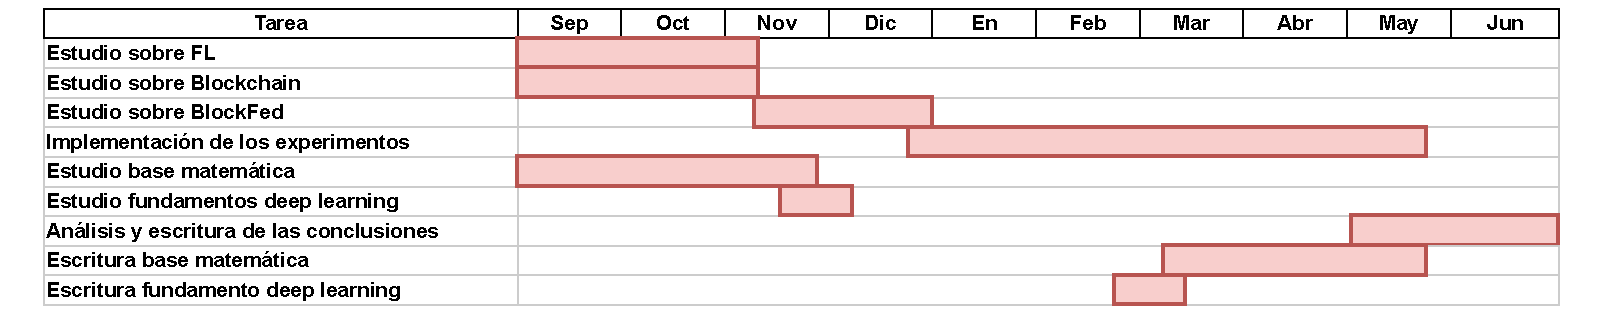
\includegraphics[width=\textwidth]{figuras/gantt.pdf}
    \caption{Diagrama de Gantt mostrando la planificación temporal.}
    \label{fig:gantt}
\end{figure}
Como podemos ver se ha trabajado de manera constante durante todo el curso en este trabajo. Las primeras tareas han sido la debida documentación sobre los fundamentos matemáticos, \ac{FL}, \textit{blockchain} y la aplicabilidad de estas dos tecnologías juntas. Durante el estudio de esta última, comenzó la implementación de los experimentos y su ejecución, la cuál ha ocupado gran parte en el tiempo debido a las múltiples iteraciones realizadas para verificar nuestras hipótesis. Una vez teniendo los experimentos encaminados, se ha dedicado el resto del tiempo a la escritura de la memoria y al análisis de estos.


En total se han empleado 10 meses para realizar el proyecto.


A la hora de calcular el presupuesto se tiene en cuenta los siguientes factores:
\begin{itemize}
    \item \textbf{Coste personal:} sabiendo que el sueldo medio de un Ingeniero Informático Jr. en España asciende a 1800 euros mensuales y su cotización social media es del 32,6\%, el gasto de personal de manera mensual sería de 2670,60 euros.

    Sabiendo la duración del proyecto y los datos anteriores deducimos que el gasto de personal para este proyecto es de $10 \times 2670,60=$ \textbf{26.706 euros}.

    \item \textbf{Coste del equipo:} para la realización de los experimentos se ha usado el clúster \textit{Talos} del Instituto Andaluz de Ciencia de Datos e Inteligencia Computacional (DaSCI) que destaca por contar con 8 tarjetas gráficas NVIDIA A100 40GB. Tras una aproximación del tiempo total de ejecución, el precio del uso de este clúster en un servicio como Google Cloud asciende a \textbf{4.601,35 euros}.
\end{itemize}

Por lo tanto, el presupuesto total de este trabajo sería de \textbf{31.307,35 euros}.


\part{Fundamentos teóricos}\label{sec:preliminares}
 \chapter{Álgebra Lineal}\label{sec:algebra}
En este capítulo introduciremos conceptos básicos de álgebra lineal~\cite{Goodfellow-et-al-2016}. Se necesitará un buen entendimiento en álgebra lineal para ser capaces de trabajar con muchos algoritmos de \ac{AA}, especialmente con aquellos de \textit{deep learning}.

\section{Conceptos básicos}
En nuestro estudio del álgebra lineal nos encontraremos con distintos tipos de objetivos matemáticos:
\begin{itemize}
    \item \textbf{Escalares:} un escalar es un número o elemento de un cuerpo, a diferencia de los demás elementos que estudiaremos más adelante que se suelen componer de varios elementos.
    \item \textbf{Vectores:} un vector es un conjunto ordenado de números. Podemos referirnos a cada número del vector mediante su índice en el conjunto.
    \item \textbf{Matrices:} una matriz es un conjunto ordenado de números de dos dimensiones. Así, para referirnos a un número lo haremos mediante dos índices.
    \item \textbf{Tensores:} un algunas ocasiones necesitaremos más de dos ejes. En este caso recurriremos a los tensores, conjuntos de números organizados en una cuadrícula general con un número variable de ejes.
\end{itemize}

Una operación importante en matrices es la \textbf{transposición}. La operación transposición equivale a obtener la imagen de un espejo a través de la diagonal de la matriz. Es decir:

\begin{definition}
Dada una matriz $A$, definimos su \textbf{transpuesta}, denotada por $A^T$ verificando
    \begin{equation}
    (A^T)_{i,j} = A_{j,i}.
    \end{equation}
\end{definition}

Pese a que hayamos definido la transpuesta como una operación sobre matrices, es fácilmente aplicable a vectores viéndolos como matrices fila y a escalares viéndolos como una matriz de una sola entrada.

Es notorio mencionar que el transpuesto de un escalar es siempre él mismo, esto es $a^T=a$.

En estas estructuras podemos definir las siguientes \textbf{operaciones}:
\begin{enumerate}
    \item Dadas dos matrices $A$ y $B$ de misma dimensión, podemos definir su suma como la matriz como la suma de las matrices componente a componente, esto es:
    \begin{equation}
        C = A + B \implies C_{i,j} = A_{i,j} + B_{i,j}.
    \end{equation}
    
    \item Definimos la suma y producto de una matriz y un escalar mediante la operación componente a componente, esto es:
    \begin{equation}
        C = aA + c \implies C_{i,j} = aA_{i,j} + c.
    \end{equation}

    \item El producto matricial es una de las operaciones más usadas del álgebra lineal en el \ac{AA}.
    \begin{definition}
        Sea $A \in \mathbb{R}^{n \times m}$ y $B \in \mathbb{R}^{m \times k}$, entonces el \textbf{producto matricial} de $A$ y $B$ es una matriz $C \in \mathbb{R}^{n\times k}$ verificando
        \begin{equation}
            C_{i,j} = \sum_{k=1}^{m} A_{i,k}B_{k,j}.
        \end{equation}
    \end{definition}
\end{enumerate}

\textbf{Propiedades del producto matricial:}
\begin{enumerate}
    \item El producto matricial es distributivo:
    \begin{equation}
        A(B+C)=AB+AC.
    \end{equation}
    \item El producto matricial es asociativo:
    \begin{equation}
        (AB)C = A(BC).
    \end{equation}
    \item El producto matricial no es conmutativo:
    \begin{equation}
        AB \ne BA.
    \end{equation}
    \item La transpuesta de un producto es el producto inverso de sus transpuestas, esto es:
    \begin{equation}
        (AB)^T = B^T A^T.
    \end{equation}
\end{enumerate}

De cara a la resolución de ecuaciones lineales haremos uso de la inversión de matrices. Para ello, primero debemos de introducir el concepto de matriz identidad.

\begin{definition}
    Definimos la \textbf{matriz identidad} como aquella que no modifica ningún vector cuando es multiplicado por ella. La matriz identidad de dimensión n quedará denotada por $I_n \in R^{n \times n}$ y verifica que
    \begin{equation}
        \forall x \in R^{n}, I_nx = x.
    \end{equation}
    Esta matriz se compone con una diagonal de 1 y todos sus demás elementos 0.
\end{definition}

\begin{definition}
    Dada una matriz $A \in \mathbb{R}^{n \times n}$ definimos su matriz inversa $A^{-1} \in \mathbb{R}^{n \times n}$ como aquella matriz que cumple que
    \begin{equation}
        AA^{-1}=A^{-1}A=I_n.
    \end{equation}

    Cabe destacar que dada una matriz $A \in \mathbb{R}^{n \times n}$ su matriz inversa no tiene por qué existir. También, si $A^{-1}$ es la matriz inversa de $A$, es fácil ver que
    \begin{equation}
        (A^{-1})^{-1}=A.
    \end{equation}
\end{definition}

\begin{definition}
    Se define el \textbf{determinante} de una matriz cuadrada $A \in \mathbb{R}^{n \times n}$ y se denotará por $det(A)$ a la suma de los $n!$ productos formados por los n-factores que se obtienen de multiplicar n-elementos de la matriz de tal forma que cada producto contenga un solo elemento de cada fila y de cada columna de A.
\end{definition}

También nos interesará definir unos tipos especiales de matrices bastante común en \ac{AA}:
\begin{definition}
    Diremos que una matriz $A$ es simétrica si $A = A^T$.
\end{definition}

\begin{definition}
    Diremos que una matriz $A$ es ortogonal si $A^{-1}=A^T$.
\end{definition}

\section{Sistemas Lineales de Ecuaciones}
Ahora conocemos suficiente álgebra lineal como para poder definir un sistema lineal de ecuaciones.
\begin{definition}
    Dada una matriz conocida $A \in \mathbb{R}^{m \times n}$, un vector conocido $b \in \mathbb{R}^m$ y un vector desconocido $x \in \mathbb{R}^n$ definimos un \textbf{sistema lineal de ecuaciones} como la ecuación
    \begin{equation}\label{linealeq}
        Ax=b.
    \end{equation}
    Cada elemento $x_i$ de nuestro vector desconocido $x$ es una variable que deseamos conocer.
\end{definition}

Otra forma de escribir la ecuación \ref{linealeq} de manera más explícita es:
\begin{equation}
\begin{split}
    A_{1,1}x_1 + A_{1,2}x_2 + \ldots + A_{1,n}x_n = b_1 \\
    A_{2,1}x_1 + A_{2,2}x_2 + \ldots + A_{2,n}x_n = b_2 \\
    \ldots \\
    A_{m,1}x_1 + A_{m,2}x_2 + \ldots + A_{m,n}x_n = b_m.
\end{split}
\end{equation}

Gran parte de las operaciones en el \textit{deep learning} se basan en ecuaciones de este tipo con la agregación de operaciones no lineales.

\begin{definition}
    Dado un conjunto de vectores $\{v^{(1)}, \ldots, v^{(n)} \}$ diremos que son \textbf{linealmente independientes} si dado un vector del conjunto, no se puede expresar como combinación lineal de los demás vectores. Esto es:
    \begin{equation}
        \nexists \alpha_j \ / \ v^{(i)} = \sum_{k=1}^n \alpha_k v^{(k)},\  k \ne i.
    \end{equation}
\end{definition}

\section{Normas}
Otro concepto muy usado en el \textit{deep learning} son las normas de vectores y matrices. Las normas son funciones que llevan vectores a escalares no negativos. De manera intuitiva se podría ver la norma de un vector $x$ como la distancia desde el origen hasta $x$. De manera más rigurosa:

\begin{definition}
    Una norma es una función $f: \mathbb{R}^n \to \mathbb{R}^+_0$ tal que:
    \begin{enumerate}
        \item $f(x) = 0 \implies x = 0$
        \item $\forall y \in \mathbb{R}^n, f(x + y) \le f(x) + f(y)$ (desigualdad triangular)
        \item $\forall \alpha \in \mathbb{R}, f(\alpha x)=|\alpha|f(x)$
    \end{enumerate}
\end{definition}

\begin{definition}
    Sea $x \in \mathbb{R}^n$, se define la norma $L^p$ con $p \in [1, \infty)$ de $x$ como:
    \begin{equation}
        || x ||_p = (\sum_{i=1}^n |x_i|^p)^\frac{1}{p}.
    \end{equation}
\end{definition}

Algunos casos particulares de la norma $L^p$ son:
\begin{enumerate}
    \item \textbf{Norma euclídea:} es el caso cuando $p=2$. Es la medida más usada en el \ac{AA} y se suele denotar como $||x||$ por simplicidad. Con bastante frecuencia mediremos su cuadrado debido a su sencillez de cálculo, pues es fácil ver que $||x||^2=xx^T$.
    \item \textbf{Norma $L^1$:} también bastante usada se trata del caso $p=1$:
    \begin{equation}
        ||x||_1 = \sum_{i=1}^n |x_i|.
    \end{equation}
    \item \textbf{Norma $L^\infty$:} también conocida como \textbf{norma del máximo} está definida mediante:
    \begin{equation}
        ||x||_\infty = \max_i |x_i|.
    \end{equation}
\end{enumerate}

\section{Descomposición en autovalores}
Muchos objetos matemáticos pueden ser mejor comprendidos separándolos en partes. Por ejemplo, los números enteros pueden ser vistos como una descomposición en números primos. En el caso de las matrices, una de las descomposiciones más usadas es en \textbf{autovalores} o \textbf{valores propios} y los autovectores o vectores propios.

\begin{definition}
    Un vector $v \in \mathbb{R}^n$ y un escalar $\lambda \in \mathbb{R}$ se dirán que son un \textbf{vector propio} y un \textbf{valor propio} respectivamente de una matriz cuadrada $A \in \mathbb{R}^{n \times n}$ si se verifica que
    \begin{equation}
        Av=\lambda v.
    \end{equation}
\end{definition}

\begin{proposition}
Si $v$ es un vector propio de una matriz cuadrada $A$, entonces también lo será $sv$ con $s \in \mathbb{R}, s \ne 0$. Es más, $v$ y $sv$ comparten el mismo valor propio:
\begin{equation}
    Av = \lambda v \implies A(sv) = \lambda (sv).
\end{equation}
\end{proposition}

\begin{proposition}
    Dada una matriz cuadrada $A$, entonces su determinante $det(A)$ se corresponde con el producto de sus valores propios:
    \begin{equation}
        det(A) = \prod_{i} \lambda_i.
    \end{equation}
\end{proposition}

Veamos la descomposición matricial que se produce mediante este tipo de vectores. Para ello supongamos que nuestra matriz $A$ tiene $n$ vectores propios linealmente independientes $\{v^{(1)}, \ldots, v^{(n)} \}$ asociados a los valores propios $\{ \lambda_1, \ldots, \lambda_n \}$. Podemos unir estos vectores en una matriz $V$ con un vector propio por columna: 
\begin{equation}
    V = [v^{(1)}, \ldots, v^{(n)}].
\end{equation}
Del mismo modo, podemos unir los valores propios en un vector denotado por $\lambda$. Entonces:
\begin{proposition}
    La \textbf{descomposición en valores propios} de $A$ viene dada por
    \begin{equation}
        A = V diag(\lambda)V^{-1}.
    \end{equation}
\end{proposition}

Un problema surge cuando dada una matriz queremos buscar sus vectores y valores propios. Sin embargo, en el caso de que una matriz sea simétrica, el cuál es un caso bastante común en \ac{AA}, esta puede ser descompuesta usando solo valores propios y vectores propios de números reales.

\begin{proposition}
    Toda matriz $A$ simétrica puede descomponerse en valores propios reales de la forma:
    \begin{equation}
        A = Q \Lambda Q^T
    \end{equation}
    donde $Q$ es una matriz ortogonal compuesta de los vectores propios de $A$ y $\Lambda$ es una matriz diagonal.
\end{proposition}

Mediante el uso de los valores propios de una matriz $A$ podemos clasificar las matrices en:
\begin{itemize}
    \item \textbf{Definida positiva:} si $\lambda_i > 0\ \forall i \in {1, \ldots, n}$.
    \item \textbf{Semidefinida positiva:} si $\lambda_i \ge 0\ \forall i \in {1, \ldots, n}$.
    \item \textbf{Definida negativa:} si $\lambda_i < 0\ \forall i \in {1, \ldots, n}$.
    \item \textbf{Semidefinida negativa:} si $\lambda_i \le 0\ \forall i \in {1, \ldots, n}$.
\end{itemize}

Cabe destacar que dada una matriz $A$ no tiene por qué ser clasificada en uno de los casos anteriores. Sin embargo es interesante pues si una matriz $A$ es semidefinida positiva entonces podemos garantizar que $x^TAx \ge 0, \forall x$ lo cual es un requisito en ciertos algoritmos de \ac{AA}.

 \chapter{Probabilidad e Inferencia Estadística}\label{sec:inferencia}
En este capítulo desarrollaremos la Teoría de la Probabilidad y la Teoría de la Información de una forma muy básica con el objetivo de facilitar la comprensión del resto del trabajo~\cite{Goodfellow-et-al-2016}.

La teoría de la probabilidad es un marco de trabajo matemático para representar la incertidumbre de los hechos. Nos proporciona tanto métodos para cuantificar la incertidumbre cómo axiomas para derivar nuevos enunciados. En la \ac{IA}, usamos la teoría de la probabilidad principalmente de dos maneras. Primero, las leyes de la probabilidad nos indican cómo un sistema de \ac{IA} debería de razonar, de forma que diseñamos nuestros algoritmos para calcular o aproximar varias expresiones derivadas usando la teoría de la probabilidad. Segundo, podemos usar probabilidad y estadística para analizar de manera teórica el comportamiento de sistemas de \ac{IA}.

Mientras que la teoría de la probabilidad nos permite enunciar con incertidumbre y razonar en la presencia de esta, la teoría de la información nos permite cuantificar la cantidad de incertidumbre en una distribución de probabilidad.

\section{Variables aleatorias}
Para la definición de \ac{v.a.} necesitamos introducir conceptos básicos de teoría de la medida~\cite{ross-2019}.

La primera definición básica para la teoría de la probabilidad es el concepto de $\sigma$-álgebra que nos servirá de base para construir los demás conceptos.

\begin{definition}
    Una familia de subconjuntos de $X$, denotada por $\Sigma$, se dirá que es una \textbf{$\sigma$-álgebra} sobre $X$ si se cumplen las siguientes propiedades:
    \begin{enumerate}
        \item El conjunto vacío $\emptyset$ es un elemento de $\Sigma$.
        \item Si $A$ es un elemento de $\Sigma$, entonces el complementario de $A$, $\bar{A}=\Sigma \diagdown A$ también pertenece a $\Sigma$.
        \item Sea $A_1, A_2, \ldots$ una sucesión de elementos de $\Sigma$, entonces la \textbf{unión numerable} de todos los conjuntos de la sucesión también es un elemento de $\Sigma$, es decir: $\bigcup A_i \in \Sigma$.
    \end{enumerate}
\end{definition}

Una vez definido lo que es una $\sigma$-álgebra y con el concepto de función de medida de Teoría de la Medida podemos definir el espacio muestral, que contempla todos los posibles resultados y escenarios de un experimento aleatorio.

\begin{definition}
    Un \textbf{espacio muestral} se define como una tripleta $(\Omega, \mathcal{A}, \mu)$ tal que:
    \begin{enumerate}
        \item $\Omega$ es el conjunto de todos los sucesos elementales.
        \item $\mathcal{A}$ es una familia de subconjuntos de $\Omega$ tal forma una $\sigma$-álgebra.
        \item $\mu$ es una función de medida de conjuntos que permite asignar una probabilidad a los sucesos del espacio muestral.
    \end{enumerate}
\end{definition}

Este concepto es clave de cara a los espacios probabilísticos, pues será la base para su definición y se le incorporará un conjunto de sucesos de interés sobre la que se define la función de probabilidad. El concepto de espacio de probabilidad o espacio probabilístico será crucial en el desarrollo de esta sección pues a partir de este se modelizan todos los experimentos aleatorios.

\begin{definition}
    Un \textbf{espacio de probabilidad} se define como una tripleta $(\Omega, \mathcal{B}, P)$ tales que:
    \begin{enumerate}
        \item $\Omega$ es el espacio muestral (sucesos elementales).
        \item $\mathcal{B}$ es una familia de sucesos aleatorios que forma una $\sigma$-álgebra.
        \item $P$ es una función de probabilidad que asigna una probabilidad a cada uno de los sucesos.
    \end{enumerate}
\end{definition}

Para entender la definición anterior necesitaremos el concepto de función de probabilidad, la cual no es otra cosa que una extensión de función de medida verificando \textbf{Axiomas de Kolmogorov}.

\begin{definition}
    Decimos que una función de medida $P$ definida sobre una $\sigma$-álgebra $\mathcal{B}$ es una \textbf{medida o función de probabilidad} si verifica que:
    \begin{enumerate}
        \item \textbf{Axioma 1}: la función toma valores en el intervalo cerrado $[0, 1]$, es decir,
        \begin{equation}
            0 \le P(A) \le 1 \ \ \forall A \in \mathcal{B}.
        \end{equation}

        \item \textbf{Axioma 2}: la probabilidad del total es 1 y la del elemento vacío es 0, es decir,
        \begin{equation}
            P(\mathcal{B}) = 1 \ \ \ P(\emptyset) = 0.
        \end{equation}

        \item Si $A_1, A_2, \ldots$ son sucesos de $\mathcal{B}$ disjuntos dos a dos entonces la probabilidad de la unión es la suma de las probabilidades, es decir,
        \begin{equation}
            P(A_1 \cup A_2 \cup A_3 \cup \ldots) = \sum P(A_i).
        \end{equation}
    \end{enumerate}
\end{definition}

En este punto contamos con las herramientas necesarias para introducir el concepto de \ac{v.a.}.

\begin{definition}
    Una \textbf{Variable Aleatoria} (\ac{v.a.}) $X$ es una función real definida en el espacio de probabilidad $(\Omega, \mathcal{B}, P)$ asociada a un determinado experimento aleatorio, esto es
    \begin{equation}
        X: \Omega \to \mathbb{R}.
    \end{equation}

    Con respecto al número de diferentes valores que puede tomar una variable, esta será:
    \begin{enumerate}
        \item \textbf{Discreta}: toma un conjunto finito o numerable de valores.
        \item \textbf{Continua}: toma un conjunto no numerable de valores.
    \end{enumerate}
\end{definition}

\section{Distribuciones de Probabilidad}
Una \textbf{distribución de probabilidad} de una variable aleatoria es una función que asigna a cada valor posible de la \ac{v.a.} una probabilidad (es decir, un valor real entre 0 y 1) de que este suceso ocurra.

En función del tipo de \ac{v.a.} sobre el cual definamos la distribución de probabilidad podemos diferenciar dos tipos de distribuciones de probabilidad.

\subsection{Distribuciones de Probabilidad definidas sobre \ac{v.a.} discretas}
Las distribuciones de probabilidad definidas sobre \ac{v.a.} discretas se definen mediante la \textbf{\ac{f.m.p.}}. Esta función asocia a cada punto del espacio muestral una probabilidad de que el suceso ocurra.

\begin{definition}
    La \textbf{función masa de probabilidad (\ac{f.m.p.}) $P$} definida sobre el espacio muestral $\mathcal{A}$ de una variable aleatoria $X$ asigna a cada punto $x_i \in \mathcal{A}$ (suceso) una probabilidad de que este ocurra, es decir,
    \begin{equation}
        P(x_i) = p_i
    \end{equation}

    donde $p_i$ es la probabilidad del suceso $X=x_i$.
\end{definition}

Una \ac{f.m.p.} verifica las siguientes propiedades:
\begin{proposition}
    Sea $P$ una función masa de probabilidad definida sobre una variable aleatoria discreta $X$, entonces:
    \begin{enumerate}
        \item El dominio de $P$ serán todos los posibles valores de $X$.
        \item $0 \le P(x) \le 1 \forall x \in X$. Así, una probabilidad de 0 indicará un suceso imposible, es decir, $X$ no puede tomar ese valor. Una probabilidad de 1 indicará un suceso seguro, es decir, $X$ siempre tomará ese valor.
        \item $\sum_{x \in X}P(x) = 1$. Esta propiedad se conoce como \textbf{normalización} y es fundamental para cumplir los axiomas de Kolmogorov pues de no ser así podríamos tener sucesos con probabilidad mayor que 1 o que la probabilidad del total no fuese 1.
    \end{enumerate}
\end{proposition}


\subsection{Distribuciones de Probabilidad definidas sobre \ac{v.a.} continuas}
En el caso de las distribuciones de probabilidad definidas sobre una \ac{v.a.} continua utilizamos la noción de \ac{f.d.p.} para describirlas.

\begin{definition}
    Una función $p$ se dice que es una \textbf{función de densidad de probabilidad (\ac{f.d.p.})} sobre una \ac{v.a.} continua $X$ si cumple que:
    \begin{itemize}
        \item El dominio de $p$ son todos los posibles valores de $X$.
        \item $p(x) \le 1\ \forall x \in X$.
        \item $\int_X p(x) dx = 1$.
    \end{itemize}
\end{definition}

En contraposición con la \ac{f.m.p.}, esta función no devuelve la probabilidad para un determinado punto del espacio muestra si no que devuelve la posibilidad de pertenecer a una región infinitesimal de volumen $dx$.

\begin{proposition}
    Para conocer la probabilidad de que nuestra \ac{v.a.} $X$ tome valores en un intervalo concreto, bastaría con integrar la \ac{f.d.p.} en dicho intervalo. En el caso univariante y suponiendo que nuestra variable toma valores reales se podría denotar de la siguiente manera:
    \begin{equation}
        P(x \in [a,b]) = P(a \le x \le b) = \int_a^bp(x)dx = \int_{[a,b]}p(x)dx.
    \end{equation}
\end{proposition}

\section{Probabilidad Marginal}
A veces, conocemos la distribución de probabilidad de una distribución sobre un conjunto de varias variables pero nos interesa conocer la distribución sobre un subconjunto de ellas. La distribución resultante sería conocida como \textbf{distribución marginal de probabilidad} del subconjunto de variables elegidas.

A continuación mostramos como obtener las probabilidad marginales:
\begin{enumerate}
    \item \textbf{Caso discreto}: consideraremos las \ac{v.a.} discretas $X$ e $Y$ y su función de probabilidad conjunta $P(X,Y)$. Para obtener la distribución marginal de cualquiera de las \ac{v.a.} bastaría con considerar la regla de la suma para la otra variable. Esto es,
    \begin{equation}
        \forall x \in X,\ P(X=x)= \sum_y P(X=x, Y=y).
    \end{equation}

    \item \textbf{Caso continuo}: para \ac{v.a.} continuas $X$ e $Y$, conocida la función de densidad de probabilidad $p(X, Y)$. Para conocer la marginal respecto a una de sus variables, usaremos la integración en la otra variable. Es decir,
    \begin{equation}
        p(X) = \int_Y p(x, y)dy.
    \end{equation}
\end{enumerate}

\section{Probabilidad Condicionada}
En múltiples ecuaciones nos interesará conocer la probabilidad de que un suceso ocurra en el caso en el que otro haya ocurrido. A esta probabilidad se le conoce como \textbf{probabilidad condicionada}. Denotamos a la probabilidad de que $X=x$ cuando sabemos que $Y=y$ como $P(X=x|Y=y)$. Esta probabilidad se calcula mediante la siguiente expresión:
\begin{equation}
    P(X=x|Y=y) = \frac{P(X=x,Y=y)}{P(Y=y)}
\end{equation}

donde $P(Y=y)$ es la probabilidad marginal de que la variable $Y$ tome el valor $y$.

\section{Conceptos y Resultados básicos de Probabilidad}
Un resultado elemental de la Teoría de la Probabilidad que nos resultará muy útil es la conocida \textbf{Regla de la Cadena}:
\begin{proposition}
    \textbf{Regla de la Cadena}. Toda probabilidad conjunta sobre un conjunto de \ac{v.a.} puede ser descompuesta en distribuciones condicionales sobre una sola variable.
\end{proposition}

\begin{proof}
    La demostración de esta proposición se puede decir que es una consecuencia directa de la definición de probabilidad condicionada. Aplicando de forma sucesiva obtenemos la siguiente descomposición:
    \begin{equation}
        P(X^{(1)}, X^{(2)}, \ldots, X^{(n)}) = P(X^{(1)}) \prod_{i=2}^n P(X^{(i)}|X^{(1)}, \ldots, X^{(i-1)}).
    \end{equation}
\end{proof}

Otro concepto básico es el concepto de independencia entre dos \ac{v.a.}.
\begin{definition}
    Dadas dos \ac{v.a.} $X$ e $Y$, diremos que son \textbf{independientes} si la distribución de probabilidad conjunta se puede descomponer como el producto de de las probabilidades de cada variable. Esto es,
    \begin{equation}
        P(X=x, Y=y)=P(X=x)P(Y=y)\ \ \forall x \in X, y \in Y.
    \end{equation}
\end{definition}

Diremos que un conjunto de \ac{v.a.} son independientes cuando las variables lo son dos a dos.

De cara a los próximos estudios estadísticos y probabilísticos de la muestra de una \ac{v.a.} nos van a resultar necesarias las siguientes medidas:
\begin{itemize}
    \item \textbf{Esperanza matemática}: se define la esperanza matemática de una función $f$ sobre una distribución de probabilidad $P(X)$ como el valor medio que toma $f$ cuando la \ac{v.a.} $X$ sigue la distribución P. Dicho de manera formal:
    
    \begin{definition}
        Se define la \textbf{esperanza matemática} en el caso discreto como
        \begin{equation}
            E[f(X)]=\sum_X P(X)f(X).
        \end{equation}
    \end{definition}
    
    \begin{definition}
        Se define la \textbf{esperanza matemática} en el caso continuo como
        \begin{equation}
            E[f(X)]=\int_X P(x)f(x)dx.
        \end{equation}
    \end{definition}

    \item \textbf{Varianza}: nos da una medida de la dispersión de los datos. Formalmente se puede definir de la siguiente manera:
    \begin{definition}
        Se define la \textbf{varianza} de una \ac{v.a.} como
        \begin{equation}
            Var(f(X)) = E[(f(X) - E[f(X)])^2].
        \end{equation}
        Dado que la varianza se define como la esperanza matemática del cuadrado de una función es directo ver que por definición la varianza siempre será no negativa.
    \end{definition}

    \item \textbf{Covarianza}: nos da una medida sobre cómo de relacionadas están dos \ac{v.a.} de forma lineal. Formalmente se puede definir de la siguiente manera.
    \begin{definition}
        Se define la \textbf{covarianza} entre una función $f(X)$ y una función $g(Y)$ con respecto a una distribución de probabilidad $P$ como
        \begin{equation}
            Cov(f(X), g(Y))=E[(f(X) - E[f(X)])(g(Y) - E[g(Y)])].
        \end{equation}
    \end{definition}

    A partir de esta definición, cuando tenemos un vector aleatorio $X \in \mathbb{R}$ definimos la \textbf{matriz de covarianzas} cómo la matriz $n \times n$ que satisface que
    \begin{equation}
        Cov(X)_{i, j} = Cov(X^{(i)}, X^{(j)}).
    \end{equation}

    Claramente esta matriz es simétrica y su diagonal está compuesta por las varianzas de las componentes del vector aleatorio.
\end{itemize}

\section{Probabilidad Bayesiana}
En ocasiones, dadas dos variables aleatorias $X$ e $Y$, nos vemos en el caso de conocer $P(Y | X)$ y queremos conocer $P(X | Y)$.

A esta última probabilidad se le conoce como probabilidad posterior y a su estudio se le conoce cómo Probabilidad Bayesiana Objetiva, la cuál es de gran importancia pues una gran cantidad de procedimientos de \ac{AA} se basan en ella~\cite{gelman-2004}.

Para comenzar a desarrollar esta teoría comenzaremos enunciando el famoso \textbf{Teorema de Bayes}, que es el principio de la teoría y que nos permite calculas la probabilidad posterior deseada conociendo $P(X)$ de la siguiente forma.
\begin{theorem}
    \textbf{Teorema de Bayes}: dadas $X$ e $Y$ dos variables aleatorias, se cumple la siguiente igualdad:
    \begin{equation}
        P(X | Y) = \frac{P(Y | X)P(X)}{P(Y)}.
    \end{equation}
\end{theorem}

Este teorema nos resultará de gran utilidad en la conocida inferencia Bayesiana, de la cuál se hace uso en \textit{deep learning}.

\section{Teoría de la Información}
La teoría de la información es una rama de las matemáticas aplicadas que gira entorno cuantificar cuanta información contiene una señal. Originalmente fue inventada para estudiar cómo mandar mensajes sobre un canal ruidoso, tales como una transmisión por radio. Esta rama cuenta con numerosas aplicaciones en la ingeniería informática, sin embargo nosotros nos centraremos en su aplicación para caracterizar distribuciones de probabilidad o para cuantificar la similitud entre estas.

\begin{definition}
    Se define el concepto de \textbf{autoinformación} de un suceso o evento $X=x$ siendo $X$ una \ac{v.a.} bajo una cierta distribución de probabilidad $P$ como
    \begin{equation}
        I(x) = -\log P(x).
    \end{equation}
\end{definition}

Si nos fijamos, esta definición se centra en trabajar con un único resultado. Con el fin de extender este concepto introducimos la conocida \textbf{entropía de Shannon}.

\begin{definition}
    Definimos la \textbf{entropía de Shannon} para medir la incertidumbre en toda la distribución de probabilidad como
    \begin{equation}
        H(X)=E[I(X)]=-E[\log P(X)] = H(P).
    \end{equation}
    En el caso de que la distribución de nuestra \ac{v.a.} $X$ sea continua, la entropía de Shannon recibirá el nombre de \textbf{entropía diferencial}.
\end{definition}

En el caso de que tengamos dos distribuciones de probabilidad diferentes, $P(X)$ y $Q(X)$, sobre la misma \ac{v.a.} $X$, podemos medir cómo de distintas son estas dos distribuciones usando la divergencia de Kullback-Leibler.

\begin{definition}
    En el contexto anterior, se define la \textbf{divergencia de Kullback-Leibler (divergencia KL)} como
    \begin{equation}
        D_{KL}(P || Q) = E[\log \frac{P(x)}{Q(x)}] = E[\log P(x) - \log Q(x)].
    \end{equation}
\end{definition}

Esta medida se puede simplificar mediante la siguiente medida.

\begin{definition}
    En el contexto anterior, se define la \textbf{entropía cruzada} como
    \begin{equation}
        H(P, Q) = - E_{X \sim P} [\log Q(X)].
    \end{equation}
\end{definition}

\begin{proposition}
    Otra definición alternativa de la entropía cruzada es
    \begin{equation}
        H(P, Q) = H(P) + D_{KL}(P || Q).
    \end{equation}
\end{proposition}

Esta nueva noción es interesante pues minimizar la entropía cruzada respecto a la distribución $Q$ es equivalente a minimizar la divergencia KL, dado que $Q$ no participa en el término omitido.

\section{Estimación de Máxima Verosimilitud}
Durante el estudio de los experimentos aleatorios~\cite{garthwaite-2002}, muchas veces querremos obtener conclusiones acerca del comportamiento de una o varias varías características de nuestra población basándonos en la observación de las mismas en un subconjunto de la población original. La inferencia estadística se centra en resolver este tipo de problemas.

En todo problema de inferencia estadística existen usa serie de elementos base del problema:
\begin{itemize}
    \item \textbf{La población}: es el conjunto de elementos en el que se pretende estudiar una determinada característica.
    \item \textbf{La característica que se desea estudiar}: se suele representar por la \ac{v.a.} que la cuantifica.
    \item \textbf{La muestra de la que se dispone para el estudio}: es un subconjunto de la población sobre el que se va a estudiar la característica para inferir las conclusiones.
\end{itemize}

Normalmente basándonos en la muestra observada intentaremos descubrir la distribución desconocida $F$ de la \ac{v.a.} involucrada en el problema. A $F$ se le conocerá por el nombre de \textbf{distribución teórica}. Según el conocimiento previo que se tenga sobre la distribución teórica se pueden plantear dos situaciones:

\begin{enumerate}
    \item Se conoce la forma de la función de distribución teórica salvo uno o varios parámetros, es decir, se sabe que $F$ pertenece a la familia de funciones de distribuciones
    \begin{equation}
        F \in \{ F_\theta, \theta \in \Theta \},
    \end{equation}
    donde $F_\theta$ tiene una forma funcional fija y conocida dependiente de uno o varios parámetros $\theta$, que se mueve dentro de $\Theta \subset \mathbb{R}^k$ conocido como espacio paramétrico. A este caso se le conoce como \textbf{inferencia paramétrica}.
    \item No se conoce nada acerca de $F$ salvo aspectos muy generales como que la \ac{v.a.} sea discreta o continua, la existencia o no existencia de momentos o aspectos similares. A este caso se le conoce como\textbf{inferencia no paramétrica}.
\end{enumerate}

Nosotros, de cara a las futuras aplicaciones en \ac{AA} nos centraremos en el primer caso, en la \textbf{inferencia paramétrica}. Además nos centraremos en la estimación puntual, es decir, buscar valores concretos $\theta$ dentro de nuestro espacio paramétrico $\Theta$.

Primero hablaremos de la muestra que queremos estudiar y le aplicaremos algunas restricciones que nos harán más cómodo trabajar con ella.

\begin{definition}
    Definimos una \textbf{muestra aleatoria simple}, de tamaño $n$, de una \ac{v.a.} $X$ con distribución teórica $F$, como un vector $(X_1, \ldots, X_n)$ formado por $n$ \ac{v.a.} \ac{i.i.d.}, es decir, con función de distribución común $F$.
\end{definition}

La ventaja de trabajar con \ac{v.a.} \ac{i.i.d.} es que la función de distribución conjunta del vector aleatorio formado por dichas variables será igual al producto de la distribuciones marginales de cada una de ellas, que al tener la misma distribución se tiene que
\begin{equation}
    F_{(X_1, \ldots, X_n)}(x_1, \ldots, x_n) = F_{X_1}(x_1)\ldots F_{X_n}(x_n) = \prod_{i=1}^n F_X(x_i), \quad (x_1, \ldots, x_n) \in \mathbb{R}^n.
\end{equation}

\begin{definition}
    Definimos el concepto de \textbf{estimador}, $T(X_1, \ldots, X_n)$ cómo una función que toma la muestra y devuelve valores del espacio paramétrico, es decir,
    \begin{equation}
        T: X^n \to \Theta.
    \end{equation}
\end{definition}

\begin{definition}
    Un estimador $T(X_1, \ldots, X_n)$ de $\theta$ se dice insesgado o centrado en el parámetro $\theta$ si
    \begin{equation}
         E_\theta[T(X_1, \ldots, X_n)] = \theta , \quad \forall \theta \in \Theta.
    \end{equation}
\end{definition}

Nuestro objetivo será encontrar un estimador con propiedades suficientemente buenas. Como vemos la definición anterior no plantea apenas ninguna condición para que una función sea un estimador, es por tanto que debemos de imponer restricciones a este. Para ello daremos la noción de función de verosimilitud.

\begin{definition}
    Sea $X$ una \ac{v.a.} con distribución en una familia paramétrica de distribuciones $\{ F_\theta, \theta \in \Theta \}$. Sea $f_\theta(x)$ la \ac{f.m.p.} o la \ac{f.d.p.} de $X$. Sea $X_1, \ldots, X_n$ una muestra aleatoria simple de $X$ y $f^n_\theta(x_1, \ldots, x_n)$ su \ac{f.m.p.} o \ac{f.d.p.} conjunta con $\theta \in \Theta$. Para cada realización muestral se define la  \textbf{función de verosimilitud} asociada a dichos valores de la muestra como una función de $\theta$ de la siguiente forma:
    \begin{equation}
        L_{x_1, \ldots, x_n}: \Theta \to \mathbb{R}^+ \cup \{0\} 
    \end{equation}
    \begin{equation}
        L_{x_1, \ldots, x_n}(\theta) =  f_\theta^n(x_1, \ldots, x_n).
    \end{equation}
\end{definition}

\begin{definition}
    En las condiciones de la definición previa, se define el \textbf{estimador de máxima verosimilitud} de $\theta$ como aquel estimador $\hat{\theta}(X_1, \ldots, X_n)$ que verifica que
    \begin{equation}
        \forall (x_1, \ldots, x_n) \in X^n, \quad L_{x_1, \ldots, x_n}(\hat{\theta}(x_1, \ldots, x_n))= \max_{\theta \in \Theta}L_{x_1, \ldots, x_n}(\theta).
    \end{equation}
\end{definition}

Podemos ver este este estimador de manera intuitiva como aquel estimador que, dada una muestra, nos da el parámetro $\theta$ que hace que sea más probable observar los datos de la muestra. Además este estimador es muy interesante porque cuenta con muy buenas propiedades, veamos algunas de ellas.

\begin{proposition}
    Bajo condiciones bastantes generales, si las ecuaciones de verosimilitud tienen solución única, $\hat{\theta}(X_1, \ldots, X_n)$, esta solución es fuertemente consistente, es decir, cuando la muestra tiende a infinito, el estimador converge al parámetro de forma casi segura.
    \begin{equation}
        \hat{\theta}(X_1, \ldots, X_n) \xrightarrow[n \to \infty]{c.s.} \theta, \quad \forall \theta \in \Theta
    \end{equation}
\end{proposition}

\begin{theorem}
    \textbf{Teorema de invarianza de Zehna}: sea $X$ una \ac{v.a.} con distribución en una familia paramétrica de distribuciones $\{F_\theta, \theta \in \Theta \}$. Sea $X_1, \ldots, X_n$ una muestra aleatoria simple de $X$. Sea $g$ una función medible. Si $\hat{\theta}(X_1, \ldots, X_n)$ es el estimador de máximo verosimilitud de $\theta$, entonces $g(\hat{\theta}(X_1, \ldots, X_n))$ lo será de $g(\theta)$.
\end{theorem}
Estas propiedades harán del estimador de máximo verosimilitud uno muy deseable a calcular. Es bastante común en el \textit{deep learning} desear minimizar la función negativa de la función de verosimilitud o la entropía cruzada con el fin de encontrar los pesos (o en este caso los parámetros) de nuestro modelo. Esto implica un problema de minimización, por lo que estudiaremos métodos para ello a continuación.

 \chapter{Optimización No Lineal}\label{sec:optim}
Gran parte de los problemas de \ac{AA} consisten en minimizar una función de pérdida respecto a una serie de parámetros. En este capítulo estudiaremos algunas técnicas para resolver problemas de optimización no restringida en dimensión finita~\cite{Luenberger-1969, Spelluci-1993, polyak-1987}. Empezaremos formulando el problema. 

Dada una función $f: \mathcal{D} \subset \mathbb{R}^n \to \mathbb{R}$; $f \in C^1(\mathcal{D})$ y $\mathcal{D}$ abierto, buscamos un mínimo (local) $x^*$ de $f$. Escribiremos este problema cómo:
\begin{equation}\label{minization}
    \min_{x \in \mathcal{D}}f(x).
\end{equation}
\begin{definition}
    Un elemento $x^*$ se dirá que es un mínimo local de $f$ si existe $\delta > 0$ tal que $f(x^*) \le f(x)$ para todo $x$ que cumpla que $||x^* - x||< \delta$.
\end{definition}

La existencia de la solución solo se puede garantizar bajo ciertas condiciones (como contraejemplo bastaría con considerar $n=1$, $f(x)=e^{x}$). Para ello primero debemos hablar de diferenciación de funciones. 
\begin{definition}
    Diremos que una función $f: \mathbb{R}^n \to \mathbb{R}$ es diferenciable en un punto $x$ si podemos encontrar un vector $a \in \mathbb{R}^n$ tal que para todo $y \in \mathbb{R}^n$,
    \begin{equation}
         f(x + y) = f(x) + <a, y> + o(y) 
    \end{equation}
    donde $<a,y>$ denota el producto escalar entre $a$ y $y$ . El vector $a$ es conocido como el gradiente de $f(x)$ en $x$ y se denota por $\nabla f(x)$.
\end{definition}
En otras palabras, una función es diferenciable en un punto $x$ si admite una aproximación lineal de primer orden en $x$. Hemos usado la notación $o$ pequeña que denota que la función $o$ es mucho más pequeña que $y$ cuando $y \to 0$. Esta definición se usa en lugar de usar un límite con el fin de dar una mayor intuición geométrica.

Está claro que el gradiente está únicamente determinado siendo sus componentes
\begin{equation}
     \nabla f_i(x) = \frac{\partial f(x)}{\partial x_i}.
\end{equation}

Supongamos que $f(x)$ es diferenciable en el segmento $[x, x+y]$. Consideramos entonces la función de una variable $\phi(t) = f(x + ty)$ y calculamos su derivada para $0 \le t \le 1$.
\begin{equation}
    \frac{\phi(t+ \varepsilon) - \phi(t)}{\varepsilon} = \frac{f(x + (t + \varepsilon)y) - f(x+ty)}{\epsilon},
\end{equation}
\begin{equation}
    = \frac{<\nabla f(x + ty), \varepsilon y> + o(\varepsilon y)}{\varepsilon}
\end{equation}
\begin{equation}\label{eq:gateaux}
    \phi'(t) = \lim_{\varepsilon \to 0} \frac{\phi(t+ \varepsilon) - \phi(t)}{\varepsilon} = <\nabla f(x + t y), y>
\end{equation}

\begin{definition}
    A la cantidad
    $$ f'(x; y) = \lim_{\varepsilon \to 0} \frac{f(x + \varepsilon y) - f(x)}{\varepsilon}$$
    se le llama derivada direccional de $f(x)$ en la dirección de $y$. Si $f(x)$ tiene derivada direccional en todas las direcciones entonces se dice que $f(x)$ es diferenciable Gateaux en el punto $x$.
\end{definition}
    
    Se deduce de la ecuación \ref{eq:gateaux} que si $f(x)$ es diferenciable en $x$, también es diferenciable Gateaux, con
\begin{equation}\label{eq:gateauxEnX}
    f'(x;y)=\phi'(0)=<\nabla f(x), y>.
\end{equation}

Además, si una función $f(x)$ es diferenciable en $[x, x+y]$, entonces, usando la ecuación \ref{eq:gateaux} y la igualdad:
\begin{equation}
    \phi(1) = \phi(0) + \int_0^1 \phi'(t)dt
\end{equation}
obtenemos que
\begin{equation}\label{eq:integralderivative}
    \begin{split}
    f(x + y) = f(x) + \int_0^1 <\nabla f(x + ty), y>dt \\
    = f(x) + <\nabla f(x), y> + \int_0^1 <\nabla f(x + ty) - \nabla f(x), y>dt.
    \end{split}
\end{equation}

\begin{definition}
    Diremos que una función $f(x)$ en $\mathcal{R}^n$ es doblemente diferenciable en un punto $x$ si es diferenciable en $x$ y si podemos encontrar una matríz simétrica $H$ de tamaño $n \times n$ tal que para todo $y \in \mathcal{R}^n$ se cumple que 
    \begin{equation}
        f(x+y) = f(x) + \langle \nabla f(x), y \rangle + \frac{\langle Hy, y \rangle}{2} + o(||y||^2).
    \end{equation}
\end{definition}

Esta matriz $H$ se conoce como Hessiana y se denotará por $\nabla^2f(x)$ o $f''(t)$. En otras palabras, una función es doblemente diferenciable en un punto $x$ si admite una aproximación cuadrática en un entorno de $x$.

Consideramos de nuevo la función escalar $\phi(t)=f(x + ty)$. Asumimos que $f$ es doblemente derivable. Procediendo de igual manera que en el caso anterior, se puede ver que
\begin{equation}
    \phi''(t) = \langle \nabla^2f(x+ty)y, y\rangle.
\end{equation}

Por lo tanto, si usamos la formula de Taylor expresando el resto en la forma de Lagrange tenemos que
\begin{equation}
    \phi(1) = \phi(0) + \phi'(0) + \frac{\phi''(\xi)}{2}, \quad 0 \le \xi \le 1
\end{equation}

y por tanto podemos encontrar un $\xi$ tal que
\begin{equation}
    f(x+y) = f(x) + \langle \nabla f(x), y \rangle + \frac{\langle \nabla^2f(x + \xi y)y, y\rangle}{2}.
\end{equation}
Una vez conocidas las nociones anteriores, podemos afirmar que una \textbf{condición suficiente para la existencia} de al menos un mínimo local es la siguiente:

\begin{proposition}
    Si existe un $x^0 \in \mathcal{D}$ tal que $\mathcal{L}_f(x^0)= \{ x \in \mathcal{D}: f(x) \le f(x^0) \}$ es compacto, (es decir, cerrado y acotado pues nos encontramos en dimensión finita) entonces $f$ tiene un mínimo local $x^*$ .
\end{proposition}

\begin{proof}
    Es consecuencia directa de la compacidad del conjunto $\mathcal{L}_f(x^0)$.
\end{proof}

Daremos también una \textbf{condición necesaria} para que un punto sea un mínimo local.

\begin{theorem}\label{firstordercond}
    Si $f$ es continuamente diferenciable en un entorno de $x^*$ y $x^*$ es un mínimo local de $f$, entonces $\nabla f(x^*) = 0$.
\end{theorem}

\begin{proof}
    Supongamos que $\nabla f(x^*) \ne 0$. Entonces podemos encontrar $\varepsilon >0$ lo suficientemente pequeño tal que
    \begin{equation}
    \begin{split}
        f(x^* - \varepsilon \nabla f(x^*)) = f(x^*) - \varepsilon ||\nabla f(x^*)||^2 + o(\varepsilon \nabla f(x^*)) \\
        = f(x^*) - \varepsilon (||\nabla f(x^*)||^2 + \varepsilon^{-1} o(\varepsilon)) < f(x^*).
    \end{split}
    \end{equation}
    Pero esto es una contradicción que $x^*$ sea un mínimo local.
\end{proof}

\begin{theorem}\label{firstsecondordercond}
    Sea  $f: \mathcal{D} \subset \mathbb{R}^n \to \mathbb{R}$; $f \in C^1(\mathcal{D})$, $\mathcal{D}$ abierto y $x^* \in \mathcal{D}$. Supongamos que $x^*$ es un mínimo local de $f$, entonces se cumple que
    \begin{equation}
        \nabla f(x^*) = 0.
    \end{equation}
     Además, si $f \in C^2(\mathcal{D})$, entonces lo siguiente también se cumple $\nabla^2 f(x^*)$ es semidefinida positiva.
\end{theorem}

\begin{proof}
    Por el teorema \ref{firstordercond}, $\nabla f(x^*)=0$ y por lo tanto para un $y$ arbitrario y un $\varepsilon$ lo suficientemente pequeño tenemos que:
    \begin{equation}
        f(x^*) \le f(x^* + \varepsilon y) = f(x^*) + \varepsilon^2 \frac{\langle \nabla^2 f(x^*)y, y \rangle}{2} + o(\varepsilon^2),
    \end{equation}
    \begin{equation}
        \langle \nabla^2 f(x^*)y, y \rangle \ge o(\varepsilon^2)/\varepsilon^2
    \end{equation}

    Pasando al límite con $\varepsilon \to 0$, obtenemos que $\langle \nabla^2 f(x^*)y, y \rangle \ge 0$. Como $y$ es arbitrario, concluimos la prueba. 
\end{proof}

Nos interesará también conocer cuando nuestro mínimo local es también global, para ello daremos una condición suficiente basada en la convexidad de nuestro dominio y nuestra función.

\begin{definition}
    $\mathcal{D} \subset \mathbb{R}^n$ se dice \textbf{convexo}, si dados dos puntos $x, y \in \mathcal{D}$ entonces $\lambda x + (1 - \lambda)y \in \mathcal{D}, \lambda \in [0, 1]$.
\end{definition}

\begin{definition}
    $f: \mathcal{D} \subset \mathbb{R}^n \to \mathcal{R}$, se dice \textbf{convexa} en $\mathcal{D}$ si dados $x, y \in \mathcal{D}$
    \begin{equation}
        \lambda f(x) + (1- \lambda)f(y) \ge f(\lambda x + (1-\lambda) y)
    \end{equation}
    con $\lambda \in [0, 1]$.
\end{definition}

\begin{theorem}
    Si $\mathcal{D} \ne \emptyset \subset \mathbb{R}^n$ es convexo y $f$ es convexa en $\mathcal{D}$, entonces todo mínimo local es también un mínimo global.
\end{theorem}

\begin{proof}
    Sea $x^*$ un mínimo local, entonces existe $\delta > 0$ tal que
    \begin{equation}
        || y - x^* || \le \delta \implies f(x^*) \le f(y).
    \end{equation}

    Supongamos $x \in \mathcal{D}$ arbitrario. Consideremos el punto $x^* + t(x - x^*) \in \mathcal{D}$ por ser convexo. Por ser $f$ convexa tenemos entonces que
    \begin{equation}
        f(x^* + t(x - x^*)) \le (1-t)f(x^*) + tf(x)
    \end{equation}

    Cogiendo un $t$ tal que $0 < t < \delta/(||x|| + ||x^*||)$ tenemos que
    \begin{equation}
        ||(x^* + t(x - x^*)) - x^*|| \le \delta.
    \end{equation}

    Por lo tanto
    \begin{equation}
        f(x^*) \le f(x^* + t(x - x^*)) \le (1-t)f(x^*) + tf(x).
    \end{equation}

    Operando tenemos que
    \begin{equation}
        f(x^*) + (t-1)f(x^*) \le tf(x)
    \end{equation}
    \begin{equation}
        tf(x^*) \le tf(x) \implies f(x^*) \le f(x),
    \end{equation}

    donde $x$ era arbitrario llegando a nuestra conclusión.
\end{proof}

\section{Descenso por el Gradiente}
Ahora vamos a analizar un método de optimización no restringida: el descenso por el gradiente. Este método, aunque raramente se implementa en su forma más pura, es un modelo para construir algoritmos más realistas, tales como el famoso descenso estocástico por el gradiente, el cual es el método por excelencia para optimizar funciones en el \ac{AA}. Daremos una prueba para su convergencia, y discutiremos los aspectos teóricos y los de implementación de estos métodos.

Supongamos que para cualquier punto $x$, podemos calcular el gradiente de una función $\nabla f(x)$. En este caso, el método más simple para minimizar $f(x)$ es el método del descenso por el gradiente, en el que, comenzando en una aproximación inicial $x^0$, construimos una sucesión
\begin{equation}\label{eq:gradientdescent}
    x^{k+1}=x^k - \gamma_k \nabla f(x^k)
\end{equation}
donde el parámetro $\gamma_k \ge 0$ es el tamaño del paso. Existen varias maneras de deducir el método \ref{eq:gradientdescent}.

Primero, si recordamos la condición necesaria de primer orden (Teorema \ref{firstordercond}) y su demostración, tenemos que si la condición no se cumple en $x$, es decir, $\nabla f(x) \ne 0$, entonces el valor de la función puede reducirse mediante el punto $x - \varepsilon \nabla f(x)$ con un valor de $\varepsilon$ lo suficientemente pequeño. Aplicando este procedimiento de manera secuencial, es como llegamos a este método.

Segundo, en un punto $x^k$ la función diferenciable $f(x)$ puede ser aproximada por la función lineal $f_k(x)=f(x^k) + <\nabla f(x^k), x - x^k>$ en términos del orden de $o(x-x^k)$. Por lo tanto, podemos buscar el mínimo de la aproximación $f_k(x)$ en un entorno de $x^k$. Por lo tanto sería natural adoptar su solución como la nueva aproximación $x^{k+1}$. 

Consideremos ahora la variante más sencilla de este método en la que $\gamma_k \equiv \gamma$:
\begin{equation}
    x^{k+1}=x^k - \gamma \nabla f(x^k).
\end{equation}
Queremos observar el comportamiento de este método bajo ciertas suposiciones sobre $f(x)$ y $\gamma$.

\begin{theorem}
    Sea $f(x)$ diferenciable en $\mathbb{R}^n$, y que el gradiente de $f(x)$ cumpla la condición de Lipschitz:
    $$ || \nabla f(x) - \nabla f(y) || \le L ||x - y||$$
    $f(x)$ esté acotada inferiormente:
    $$ f(x) \ge f^* > - \infty $$
    y que $\gamma$ cumpla que
    $$0 < \gamma < 2/L $$.

    Entonces, el método del gradiente tiende a cero:
    $$ \lim_{k \to \infty}\nabla f(x^k) = 0 $$
\end{theorem}

\begin{proof}
    Si sustituimos $x = x^k$ y $y = -\gamma \nabla f(x^k)$ en la ecuación \eqref{eq:integralderivative} y usamos la ecuación \eqref{eq:gateauxEnX} obtenemos que:
    \begin{equation}
    \begin{split}
        f(x^{k+1})=f(x^k) - \gamma || \nabla f(x^k) ||^2 - \gamma \int_0^1 <\nabla f(x^k -t \gamma \nabla f(x^k)), \nabla f(x^k)>dt \\
        \le f(x^k) - \gamma || \nabla f(x^k) ||^2 + L \gamma^2 || \nabla f(x^k) ||^2 \int_0^1 tdt \\
        = f(x^k) - \gamma (1- \frac{1}{2}L \gamma)|| \nabla f(x^k) ||^2.
    \end{split}
    \end{equation}

    Por lo tanto tenemos que:
    \begin{equation}
        f(x^{k+1}) \le f(x^k) - \gamma (1- \frac{1}{2}L \gamma)|| \nabla f(x^k) ||^2.
    \end{equation}

    Podemos sumar estas desigualdades desde 0 hasta $s$ para obtener lo siguiente:
    \begin{equation}
        f(x^{s+1}) \le f(x^0) - \gamma (1- \frac{1}{2}L \gamma) \sum_{k=0}^s || \nabla f(x^k)||^2.
    \end{equation}
    Sabiendo por \eqref{eq:integralderivative} que $\alpha = \gamma (1- \frac{1}{2}L \gamma) > 0$, podemos despejar la suma para obtener que
    \begin{equation}
        \sum_{k=0}^s || \nabla f(x^k)||^2 \le \alpha^{-1}(f(x^0) - f(x^{s+1})) \le \alpha^{-1}(f(x^0) - f^*)
    \end{equation}

    para toda $s$. Por lo tanto la suma es finita y por ello el término principal debe de tender a 0, es decir, $|| \nabla f(x^k) || \to 0$.
\end{proof}

Este método nos da una manera de obtener una sucesión que converja a un punto crítico de la función. Sin embargo debemos de recordar que el hecho de que $\nabla f(x) = 0$ si bien es una condición necesaria no es suficiente para que $x$ sea un mínimo. El contraejemplo por excelencia para este tipo de situaciones son los famosos puntos de silla. Es decir, el descenso por el gradiente puede ``quedarse atascado`` en cualquier punto estacionario, ya sea este un mínimo o un punto de silla. Además, este método no ``distingue`` entre un mínimo global o un mínimo local y no hay ningún tipo de garantía a la convergencia de un mínimo global.

Aún así, el método del descenso por el gradiente es la base para el principal método de optimización usado en el \ac{AA}, el descenso estocástico por el gradiente. En un problema de \ac{AA}, normalmente intentamos minimizar una función de pérdida o coste, que se suele calcular como la suma de esta en cada uno de los valores de la muestra que usamos. 

El descenso estocástico por el gradiente~\cite{Goodfellow-et-al-2016} es un método de optimización basado en el descenso por el gradiente ya expuesto en el que, en lugar de calcular el gradiente, se hace uso de un estimador insesgado del gradiente de la función de coste mediante el uso una muestra llamada \textit{minibatch} $\{ x^{(1)}, \ldots, x^{(m)}\}$. Formalmente sería:
\begin{equation}
    \hat{g} = \frac{1}{m}\nabla_\theta \sum_i L(f(x^{(i)}; \theta), y^{(i)})
\end{equation}
donde actualizaríamos $\theta$ en la dirección de $\hat{g}$. Aquí, $L$ es la función de coste o pérdida, $y^{(i)}$ será lo que próximamente llamemos etiqueta de $x^{(i)}$ y $f(x;\theta)$ es un funcional.
 \chapter{Operador de agregación Krum}\label{sec:krum}
Un problema común que nos encontraremos más adelante es el de agregar una serie de estimaciones de un gradiente para obtener un nuevo vector que nos permita resumir la información contenida por los vectores anteriores. Esto es, obtener una estimación del gradiente de una función mediante estimaciones previas en un algoritmo iterativo.

En nuestro caso podemos considerar que tenemos $n$ vectores, de los cuales $f$ pueden ser bizantinos, esto es, con valores arbitrarios. En cada paso $t$ de nuestro algoritmo, se considera un vector real denotado por $x_t \in \mathbb{R}^d$ de parámetros. Cada vector consiste en un valor estimado $V_p^t=G(x_t, \xi_p^t)$ del gradiente $\nabla Q(x_t)$ de la función de coste $Q$, donde $\xi_p^t$ es una variable aleatoria representando una muestra de un conjunto de datos. Sin embargo, un vector bizantino $V_b^t$ se puede desviar arbitrariamente del vector esperado.

Dadas las estimaciones podemos calcular un nuevo vector $F(V_1^t, \ldots, V_n^t)$ mediante una función determinista $F: (\mathbb{R}^d)^n \to \mathbb{R}^d$ llamada regla de agregación y los vectores estimados. Finalmente, podemos actualizar nuestros parámetros mediante la siguiente ecuación basada en el descenso estocástico por el gradiente
\begin{equation}
	x_{t+1} = x_{t} - \eta_t \cdot F(V_1^t, \ldots, V_n^t).
\end{equation}

\begin{figure}[h]
    \centering
    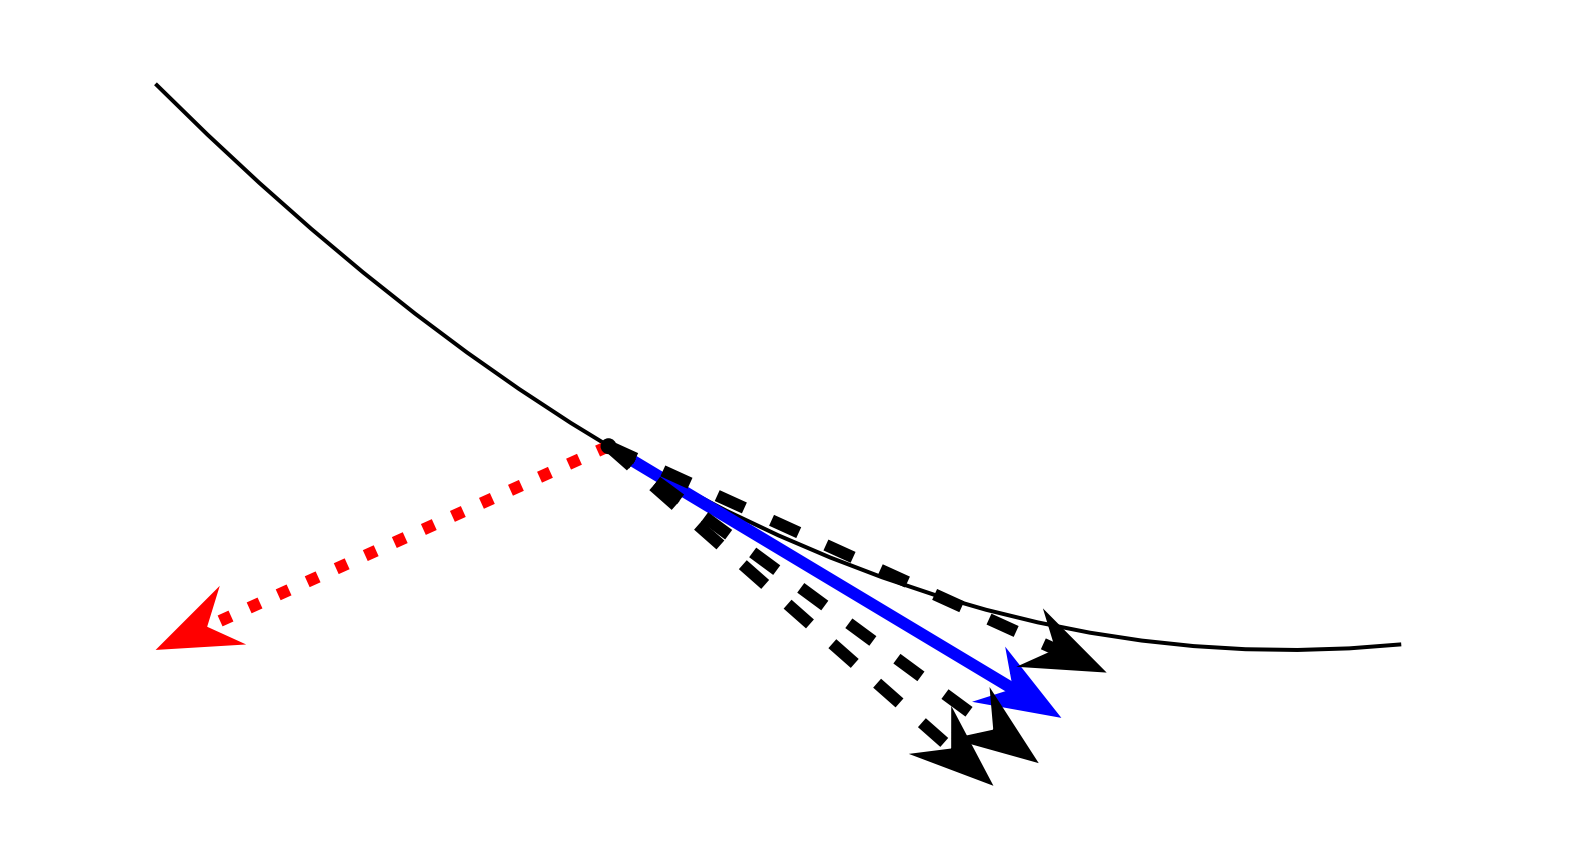
\includegraphics[width=0.8\textwidth]{figuras/krum_gradient.png}
    \caption{Las estimaciones del gradiente producidas por los estimadores correctos (flechas discontinuas negras) están distribuidas alrededor del gradiente (flecha azul sólida). Un vector bizantino puede tener un valor arbitrario (flecha roja discontinua). Fuente: \cite{krum-2017}.}
    \label{fig:krumgradient}
\end{figure}

Esperamos que los vectores no bizantinos (benignos) sean estimaciones insesgadas del gradiente $\nabla Q(x_t)$.  De manera más precisa, en cada ronda $t$, los vectores benignos $V_i^t$ son vectores aleatorios \ac{i.i.d.} con $V_i^t \sim G(x_t, \xi_i^t)$ tales que $E_{\xi_i^t}[G(x_t, \xi_i^t)] = \nabla Q(x_t)$. 

Como veremos más adelante en esta memoria, la regla de agregación más común consiste en calcular la media de los vectores. Sin embargo, ninguna combinación lineal de los vectores puede tolerar a un vector bizantino, y por tanto esta regla no es resistente a ataques bizantinos.

\begin{lemma}
	Sea $F_{lin}$ una regla de agregación de la forma $F_{lin}(V_1, \ldots, V_n)=\sum_{i=1}^n \lambda_i \cdot V_i$ donde $\lambda_i$ son escalares distintos de cero. Sea $U \in \mathbb{R}^d$. Entonces, un solo vector bizantino puede hacer que $F$ siempre compute $U$ como salida. Particularmente, un único vector bizantino puede evitar la convergencia del modelo. 
\end{lemma}

\begin{proof}
	La demostración resulta inmediata. Dado que se puede asumir que se tiene conocimiento total sobre los vectores $V_i$ y la regla de agregación $F_{lin}$ (y por tanto de los escalares $\lambda_i$), puede proponer el el vector $V_n = \frac{1}{\lambda_n}\cdot U - \sum_{i=1}^{n-1}\frac{\lambda_i}{\lambda_n}V_i$, haciendo así que $F_{lin}(V_1, \ldots, V_n)=U$.
\end{proof}

Viendo esto, nuestro objetivo es buscar una regla de agregación resistente a ataques bizantinos. De manera intuitiva, queremos que el resultado (esperado) $F$  de nuestra regla no se aleje demasiado del gradiente ''real'' $g$. Esto se puede expresar mediante el uso de una cota inferior del producto escalar del vector $F$ y $g$, así acotando el ángulo que ambos forman. Particularmente, si $E[F]$ se encuentra en una bola centrada en $g$ con radio $r$, entonces el producto escalar está acotado inferiormente por un término que implica a $\sin \alpha = r / ||g||$.

Otra condición que buscamos, aunque más técnica, es que los momentos de $F$ deben de depender de los momentos del estimador (correcto) del gradiente $G$. Esto se debe a que las cotas de los momentos de $G$ se suelen usar para controlar los efectos de la naturaleza discreta del método del descenso estocástico por el gradiente.

\begin{definition}
	Sea $0 \le \alpha < \pi/2$ cualquier ángulo, y cualquier entero $0 \le f \le n$. Sean $V_1, \ldots, V_n$ vectores aleatorios \ac{i.i.d.} en $\mathbb{R}^d$, $V_i \sim G$, con $E[G]=g$. Sean $B_1, \ldots, B_f$ vectores aleatorios en $\mathbb{R}^d$, posiblemente dependientes de los vectores $V_i$. Diremos que una regla de agregación $F$ es $(\alpha, f)$-Resistente bizantina si, para cualesquiera $1 \le j_1 < \ldots < j_f \le n$, el vector
	\begin{equation}
		F = F(V_1, \dots, \underbrace{B_1}_{j_1}, \ldots, \underbrace{B_f}_{j_f}, \ldots, V_n)
	\end{equation}
	cumple que $\langle E[F], g \rangle \ge (1-\sin \alpha) \cdot ||g||^2 > 0$ y que para $r \in \{ 2, 3, 4\}$, $E[||F||^r]$ está superiormente acotada por una combinación linear de los términos $E[||G||^1], \ldots, E[||G||^{r_{n-1}}]$ con $r_1 + \ldots + r_{n-1}=r$.
\end{definition}

\begin{figure}[h]
    \centering
    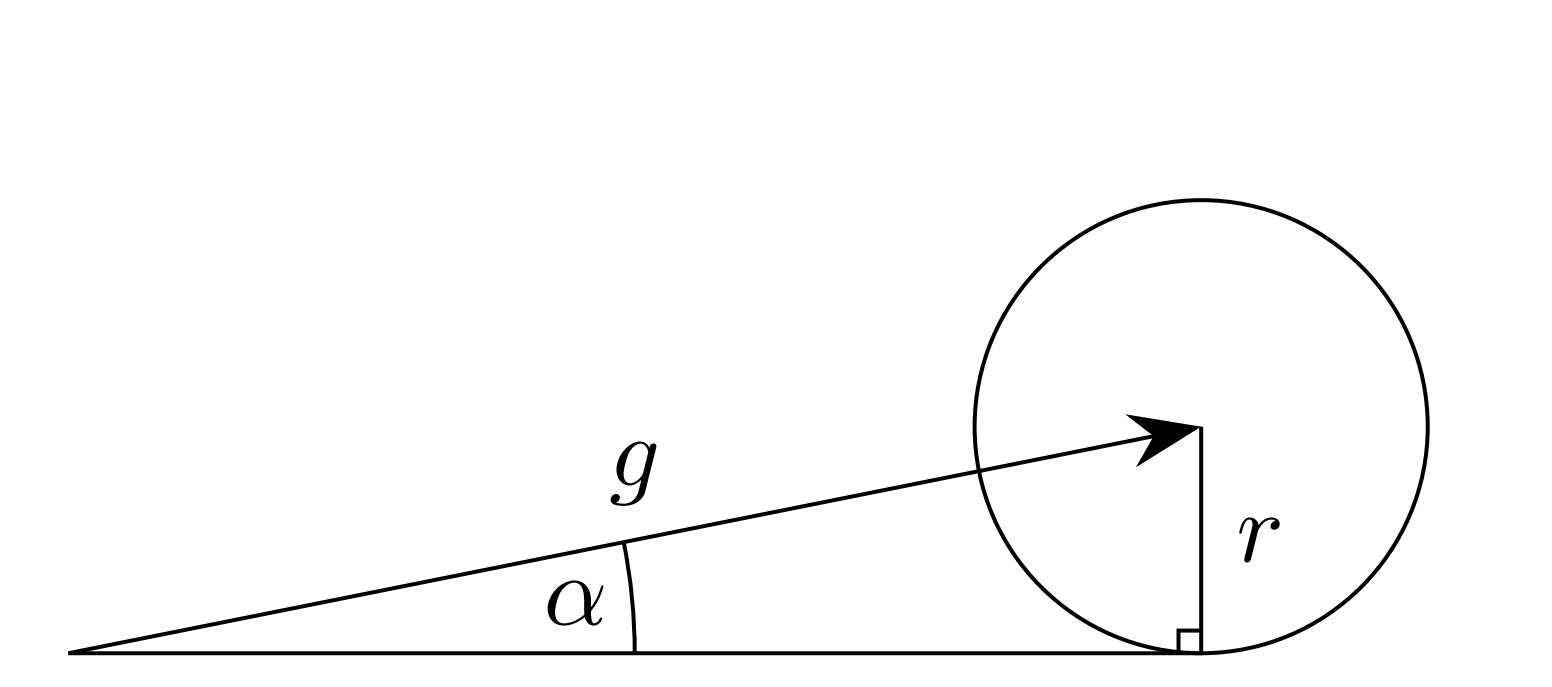
\includegraphics[width=0.8\textwidth]{figuras/krum_angle.png}
    \caption{Si $||E[F-g]|| \le r$, entonces $\langle E[F], g \rangle$ está inferiormente acotado por $(1- \sin \alpha)||g||^2$ donde $\sin \alpha= r/ ||g||$. Fuente: \cite{krum-2017}.}
    \label{fig:krumangle}
\end{figure}

Tras haber dado una definición formal de lo que es una regla de agregación resistente, procedemos a introducir la regla de agregación Krum, que cumplirá la condición ya explicada. La idea detrás de Krum consiste en que calcular el promedio puede verse también como calcular el vector que minimiza la suma de las distancias al cuadrado de los vectores $V_i$. La idea de Krum vuelve a ser la de encontrar un vector que minimice sumas de distancias a los demás vectores, pero excluyendo de estas a los vectores que estén ´´muy lejos´´ de manera que un vector bizantino no pueda forzar a la regla a escoger un vector arbitrario.

Formalmente, se define la regla de agregación Krum $KR(V_1, \ldots, V_n)$ de la siguiente manera. Para todos $i \ne j$, denotamos por $i \to j$ el hecho de que el vector $V_j$ está en el conjunto de los $n-f-2$ vectores más cercanos a $V_i$. Para cada vector $i$ se define la siguiente puntuación
\begin{equation}
	s(i) = \sum_{i \to j} ||V_i - V_j||^2.
\end{equation}
Finalmente, $KR(V_1, \ldots, V_n) = V_{i_*}$ donde $s(i_*) \le s(i)$ para todo $i$.

A continuación daremos una condición sobre $n$, $f$ y el estimador del gradiente usado para que la regla Krum sea $(\alpha, f)$-resistente bizantina.

\begin{theorem}
	Sean $V_1, \ldots, V_n$ vectores aleatorios $d$-dimensionales \ac{i.i.d.} tales que $V_i \sim G$ con $E[G]=g$ y $E[||G-g||^2]=d\sigma^2$. Sean $B_1, \ldots, B_f$ vectores aleatorios, posiblemente dependientes de los vectores $V_i$. Si $2f + 2 < n$ y $\eta(n, f)\sqrt{d}\cdot \sigma < ||g||$, donde
	\begin{equation}
		\eta(n,f) = \sqrt{2 \left( n-f + \frac{f \cdot (n-f-2) + f^2 \cdot(n-f-1)}{n-2f-2} \right)},
	\end{equation}
	
	entonces la regla de agregación Krum $KR$ es $(\alpha, f)$-resistente bizantina, donde el $\alpha$ se define como
	\begin{equation}
		\sin \alpha = \frac{\eta(n, f) \cdot \sqrt{d} \sigma}{||g||}.
	\end{equation}
\end{theorem}

\begin{proof}
	Sin perder generalidad, podemos asumir que los vectores $B_1, \ldots, B_f$ ocupan las últimas $f$ posiciones de la lista de argumentos de $KR$. Diremos que un índice es correcto si se refiere a un vector entre $V_1, \ldots, V_{n-f}$ y bizantino si se refiere a un vector entre $B_1, \ldots, B_f$. Para cada índice $i$, denotamos por $\delta_c(i)$  (o $\delta_b(i)$) a la cantidad de índices correctos (o bizantinos) $j$ tales que $i \to j$. Claramente tenemos que
	\begin{equation}\begin{split}
			\delta_c(i) + \delta_b(i) = n - f - 2 \\
			n - 2f - 2 \le \sigma_c(i) \le n-f-2 \\
			\sigma_b(i) \le f.
	\end{split}\end{equation}
	
	Nos centraremos primero en acotar el producto escalar. Empezaremos dando una cota superior de $||E[KR - g]||^2$. Recordemos que, si $j$ es correcto, entonces $E[V_j]=g$. Sea $i_*$ el índice del vector elegido por la regla Krum.
	\begin{equation}\begin{split}
			||E[KR-g]||^2 \le ||E \left( KR - \frac{1}{\delta_c(i_*)} \sum_{i_* \to j \text{ correctos}}V_j \right) ||^2 \\
			\le E[|| KR - \frac{1}{\delta_c(i_*)} \sum_{i_* \to j \text{ correctos}}V_j ||^2] \quad \text{(Desigualdad de Jensen)} \\
			\le \sum_{i \text{ correcto}} E[|| KR - \frac{1}{\delta_c(i_*)} \sum_{i_* \to j \text{ correctos}}V_j ||^2]  \mathbb{1}(i_* = i) \\
			+ \sum_{k \text{ biz}} E[||B_k - \frac{1}{\delta_c(k)} \sum_{k \to j \text{ correctos}}V_j||^2] \mathbb{1}(i_*=k)
	\end{split}\end{equation}
	
	Ahora analizamos el caso $i_* = i$ con $i$ un índice correcto.
	\begin{equation}\begin{split}
			||V_i - \frac{1}{\delta_c(i)}\sum_{i_* \to j \text{ correctos}}V_j||^2 = ||\frac{1}{\delta_c(i)}\sum_{i_* \to j \text{ correctos}}V_i - V_j||^2 \\
			\le \frac{1}{\delta_c(i)}\sum_{i_* \to j \text{ correctos}}||V_i - V_j||^2
	\end{split}\end{equation}
	
	y por tanto
	\begin{equation}\begin{split}
			E[||V_i - \frac{1}{\delta_c(i)}\sum_{i_* \to j \text{ correctos}}V_j||^2] \le \frac{1}{\delta_c(i)}\sum_{i_* \to j \text{ correctos}}E[||V_i - V_j||^2] \\
			\le 2d \sigma^2.
	\end{split}\end{equation}
	Ahora analizamos el caso $i_*=k$ siendo $k$ un índice bizantino. El hecho de que $k$ minimiza la puntuación significa que para todos los índices correctos $i$
	\begin{equation}\begin{split}
			\sum_{k \to j \text{ correctos}} ||B_k - V_j||^2 + \sum_{k \to l \text{ bizantinos}} ||B_k - B_l||^2 \\
			\le \sum_{i \to j \text{ correctos}} ||V_i - V_j||^2 + \sum_{i \to l \text{ bizantinos}} ||V_i - B_l||^2.
	\end{split}\end{equation}
	Entonces, para todo índice correcto $i$
	\begin{equation}\begin{split}
			||B_k - \frac{1}{\delta_c(k)} \sum_{k \to j \text{ correctos}}V_j||^2 \le \frac{1}{\delta_c(k)}\sum_{k \to j \text{ correctos}} ||B_k - V_j||^2 \\
			\le \frac{1}{\delta_c(k)}\sum_{i \to j \text{ correctos}} ||V_i - V_j||^2 + \frac{1}{\delta_c(k)} \underbrace{\sum_{i \to l \text{ bizantinos}} ||V_i - B_l||^2}_{D^2(i)}.
	\end{split}\end{equation}
	
	Nos fijamos a continuación en el término $D^2(i)$. Cada vector correcto $i$ tiene $n-f-2$ vecinos, y $f+1$ no vecinos. Por lo tanto, debe de existir un vector correcto $\zeta(i)$ que está más lejos de $i$ que cualquiera de sus vecinos. En particular, para cada índice bizantino $l$ tal que $i \to l$, $||V_i - B_l||^2 \le ||V_i - V_{\zeta(i)}||^2$. Por lo tanto
	\begin{equation}\begin{split}
			||B_k - \frac{1}{\delta_c(k)}\sum_{k \to j \text{ correctos}}V_j||^2 & \le \frac{1}{\delta_c(k)} \sum_{i \to j \text{ correctos}}||V_i - V_j||^2 + \frac{\delta_b(i)}{\delta_c(k)}||V_i - V_{\zeta(i)}||^2 \\
			E[||B_k - \frac{1}{\delta_c(k)}\sum_{k \to j \text{ correctos}}V_j||^2] & \le \frac{\delta_c(i)}{\delta_c(k)}2d\sigma^2 + \frac{\delta_b(i)}{\delta_c(k)} \sum_{i \ne j \text{ correctos}} E[||V_i - V_j||^2]\mathbb{1}(\zeta(i) = j) \\
			& \le \left( \frac{\delta_c(i)}{\delta_c(k)} + \frac{\delta_b(i)}{\delta_c(k)}(n-f-1) \right)2d\sigma^2 \\
			& \le \left( \frac{n-f-2}{n-2f-2} + \frac{f}{n-2f-2}\cdot (n-f-1) \right)2d\sigma^2.
	\end{split}\end{equation}
	Juntando todo obtenemos
	\begin{equation}\begin{split}
			||E[KR-g]||^2 \le (n-f)2d\sigma^2 + f \cdot \left( \frac{\delta_c(i)}{\delta_c(k)} + \frac{\delta_b(i)}{\delta_c(k)}(n-f-1) \right)2d\sigma^2 \\
			\le \left( \frac{n-f-2}{n-2f-2} + \frac{f}{n-2f-2}\cdot (n-f-1) \right)2d\sigma^2 \\
			\le \underbrace{2\left( n-f+\frac{f \cdot (n-f-2) + f^2 \cdot (n-f-1)}{n-2f-2} \right)}_{\eta^2(n,f)}d\sigma^2.
	\end{split}\end{equation}
	
	Dado que por hipótesis, $\eta(n,f)\sqrt{d}\sigma < ||g||$, entonces $E[KR]$ pertenece a la bola centrada en $g$ y con radio $\eta(n,f)\sqrt{d}\sigma$. Esto implica que
	\begin{equation}
		\langle E[KR], g\rangle \ge (||g|| - \eta(n,f)\sqrt{d}\sigma) ||g|| = (1 - \sin \alpha) ||g||^2
	\end{equation}
	y por tanto se cumple la primera propiedad para que $KR$ sea una regla $(\alpha, f)$-resistente bizantina. Ahora nos centraremos en la segunda condición.
	\begin{equation}\begin{split}
			E[||KR||^r] = \sum_{i \text{ correctos}}E[||V_i||^r]\mathbb{1}(i_*=i) +  \sum_{k \text{ bizantinos}}E[||B_k||^r]\mathbb{1}(i_*=k) \\
			\le (n-f)E[||G||^r] + \sum_{k \text{ bizantinos}}E[||B_k||^r]\mathbb{1}(i_*=k)
	\end{split}\end{equation}
	
	Denotando por $C$ a una constante genérica, cuando $i_*=k$, entonces tenemos para todos los índices correctos $i$
	\begin{equation}\begin{split}
			||B_k - \frac{1}{\delta_c(k)}\sum_{k \to j \text{ correctos}} V_j|| & \le \sqrt{\frac{1}{\delta_c(k)} \sum_{i \to j \text{ correctos}} ||V_i - V_j||^2 + \frac{\delta_b(i)}{\delta_c(k)}||V_i - V_{\zeta(i)}||^2} \\
			& \le C \cdot \left(  \sqrt{\frac{1}{\delta_c(k)}} \sum_{i \to j \text{ correctos}} ||V_i - V_j|| + \sqrt{\frac{\delta_b(i)}{\delta_c(k)}} ||V_i - V_{\zeta(i)}|| \right) \\
			& \le C \cdot \sum_{j \text{ correctos}}||V_j||\quad \text{(desigualdad triangular)}.
	\end{split}\end{equation}
	
	Donde la segunda desigualdad proviene del hecho de que las normas en dimensión finita son equivalentes. Ahora
	\begin{equation}\begin{split}
			||B_k|| & \le || B_k - \frac{1}{\delta_c(k)}\sum_{k \to i \text{ correctos}} V_j ||+ ||\frac{1}{\delta_c(k) }\sum_{k \to i \text{ correctos}} V_j|| \\
			& \le C \cdot \sum_{j \text{ correctos}}||V_j|| \\
			||B_k||^r & \le C \cdot \sum_{r_1 + \ldots + r_{n-f}=r}||V_1||^{r_1} \ldots ||V_{n-f}||^{r_{n-f}}
	\end{split}\end{equation}
	
	donde por la independencia de los $V_i$, finalmente obtenemos que $E[||KR||^r]$ está acotado superiormente por una combinación lineal de la forma $E[||V_1||^{r_1}]\ldots E[||V_{n-f}||^{r_{n-f}}]=E[||G||^{r_1}]\ldots E[||G||^{r_{n-f}}]$ con $r_1 + \ldots + r_{n-f}=r$ terminando así la prueba.
\end{proof}
 \chapter{Teoría del Aprendizaje}\label{sec:aa}
En este capítulo introduciremos los conceptos básicos del \ac{AA} para introducir posteriormente el concepto de \textit{Deep Learning}. Hablaremos del concepto de aprendizaje y de los diferentes tipos de problemas a los que se enfrenta el \ac{AA}

\section{Concepto de Aprendizaje Automático}
Un algoritmo de \ac{AA} es un algoritmo capaz de aprender información a partir de  un cierto conjunto de datos. Para saber de qué hablamos cuando hablamos de aprender podemos referirnos a \cite{mitchell-1997}, ``Un programa de ordenador se dice que aprende de una experiencia $E$ con respecto a un conjunto de tareas $T$ y medida de rendimiento $P$, si su rendimiento como tarea en $T$, medido con $P$, mejora tras conocer la experiencia $E$``. Desde el punto de vista de las tareas $T$, el \ac{AA} es interesante pues nos permite resolver una gran cantidad de tareas que son muy difíciles o incluso imposibles de resolver con programas escritos y diseñados por humanos, ya sea por el complejidad o por el tamaño de la tarea.

Otra definición interesante del concepto de aprendizaje es el de \cite{learningfromdata}. Para ello primero mencionamos los componentes del problema. Hay una entrada $x$, una función objetivo $f: \mathcal{X} \to \mathcal{Y}$, donde $\mathcal{X}$ es el espacio de todas las posibles entradas y $\mathcal{Y}$ es el espacio de los posibles resultados. Además, contamos con un conjunto de muestras $\mathcal{D} \subset \mathcal{X} \times \mathcal{Y}$ donde $y = f(x)$ si $(x, y) \in \mathcal{D}$. Finalmente, existe un algoritmo que usa el conjunto $\mathcal{D}$ para escoger una fórmula $g: \mathcal{X} \to \mathcal{Y}$ que aproxime $f$. Este algoritmo escogerá $g$ dentro de un conjunto de funciones $\mathcal{H}$.

\begin{figure}[!h]
    \centering
    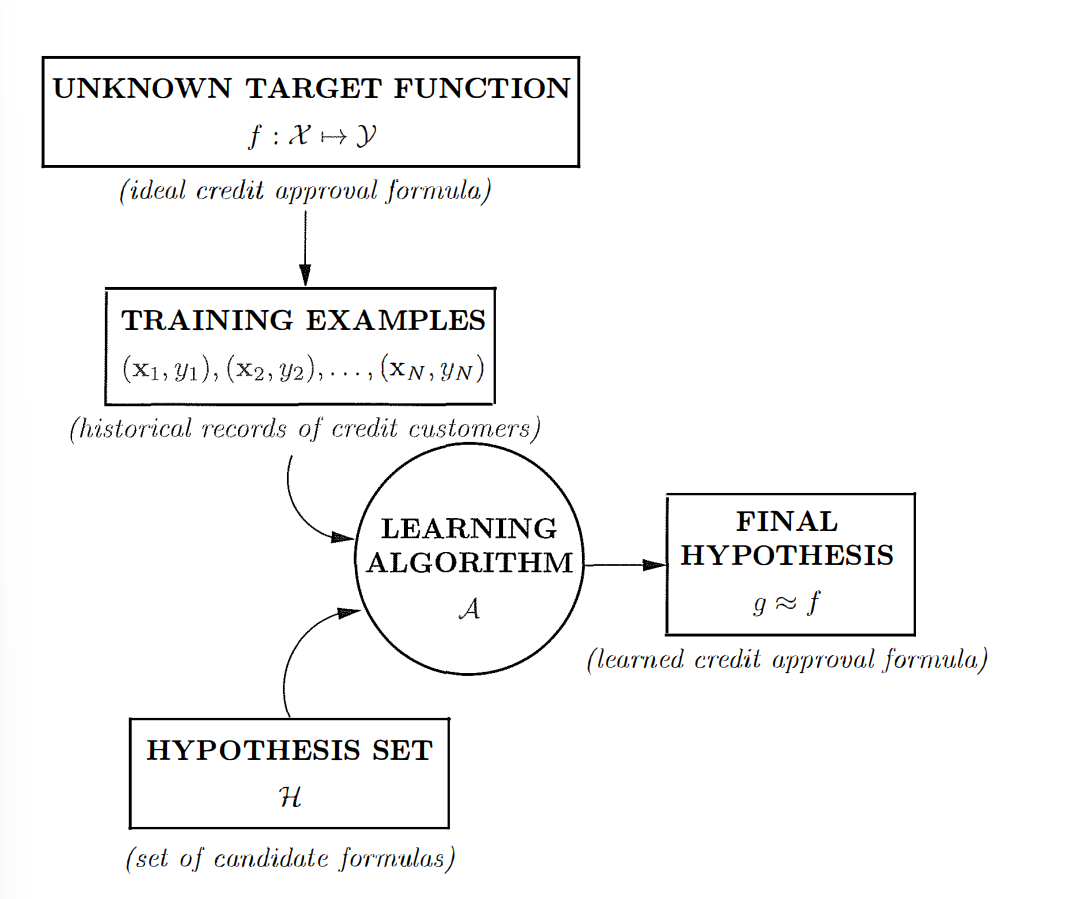
\includegraphics[width=0.8\textwidth]{figuras/learning.png}
    \caption{Escenario básico de un problema de aprendizaje. Fuente: \cite{learningfromdata}.}
    \label{fig:learningsetup}
\end{figure}

Si consideramos los múltiples componentes del problema, la función objetivo $f$ y las muestras de entrenamiento $\mathcal{D}$ están dictadas por el problema. Sin embargo, el algoritmo de aprendizaje y el conjunto de funciones en el que buscamos $\mathcal{H}$ no lo están, y son por lo tanto somos nosotros quienes las fijamos. Al conjunto $\mathcal{H}$ y al algoritmo se le refiere informalmente como el modelo de aprendizaje.

El \ac{AA} ha sido aplicado a una gran variedad de situaciones. En la literatura se pueden encontrar ejemplos:
\begin{itemize}
    \item Clasificación.
    \item Clasificación con valores perdidos.
    \item Regresión.
    \item Transcripción.
    \item Detección de anomalías.
    \item Predicción de valores perdidos.
    \item Estimación de densidad.
\end{itemize}

Con respecto a la medida de rendimiento $P$, esta debe de ser cuantitativa. La medida por excelencia en casos de clasificación es la precisión o \textit{accuracy}, definida como la proporción de muestras para las que el modelo ha producido una salida correcta. También en muchas ocasiones es útil la tasa de error, que mide la proporción de muestras para las que el modelo ha producido una salida incorrecta.

\section{Tipos de Aprendizaje Automático}
En función de la experiencia $E$, podemos clasificar los algoritmos de \ac{AA} en dos grandes grupos: algoritmos supervisados y no supervisados.
\begin{itemize}
    \item \textbf{Aprendizaje Automático No Supervisado}: cuando los datos con los que trabajamos están formados por un conjunto de datos que representa diferentes características de cada una de las muestras. Normalmente, en este caso el objetivo suele ser encontrar alguna propiedad importante para la estructura del conjunto. Un ejemplo clásico es el \textit{clustering} que consiste en agrupar los datos en subconjuntos que contengan características similares.
    \item \textbf{Aprendizaje Automático Supervisado}: cuando se tiene información de un conjunto con características y donde cada muestra tiene asociada una etiqueta. Así, el objetivo de estos problemas será encontrar la relación entre las características de una muestra y su etiqueta para poder etiquetar características futuras. Un ejemplo es el problema de clasificación.
    \item \textbf{Aprendizaje por Refuerzo}: cuando el conjunto de datos no contiene de manera explícita la salida correcta para cada entrada, sino que contiene una posible salida junto a una medida de como de adecuada esta salida es. Este tipo de aprendizaje es ideal para situaciones en las que no existe necesariamente un resultado correcto, como puede ser el problema de la conducción autónoma de vehículos.
\end{itemize}

\section{Problema de clasificación}

El problema de clasificación es el ejemplo más frecuente de aprendizaje supervisado. Consiste en, a partir de una población de entrada, clasificarla en diferentes subpoblaciones o clases. Se debe de conocer previamente el número de clases posibles, por lo que el problema consiste en decidir para cada elemento qué clase es la que mejor se ajusta a sus características observadas. Según el número de clases consideradas se puede distinguir entre:
\begin{itemize}
    \item \textbf{Clasificación Binaria}: cuando la clasificación se reduce a tan solo dos etiquetas. Se puede ver como un problema de verdadero o falso, o pertenencia o no a un subgrupo de la población.
    \item \textbf{Clasificación Multiclase}: cuando el conjunto de etiquetas es mayor que dos. En este caso se debe elegir entre todas ellas cuál es la más adecuada.
\end{itemize}

Nosotros nos centraremos en los problemas de clasificación multiclase.

\chapter{Fundamentos del Deep Learning}\label{sec:deep}
En este capítulo nos centraremos propiamente en el \textit{Deep Learning}. Para ello estudiaremos las redes neuronales prealimentadas, cómo funcionan y estudiaremos el aprendizaje basado en gradiente. Posteriormente hablaremos de redes convolucionales y concretamente de la arquitectura \texttt{EfficientNet}.

\section{Redes Neuronales Prealimentadas}
Las redes neuronales prealimentadas o \ac{MLP} son el modelo por excelencia del \textit{deep learning}~\cite{Goodfellow-et-al-2016}. El objetivo de un \ac{MLP} es el de aproximar una función $f^*$. Por ejemplo, para un clasificador, $y = f^*(x)$ lleva una entrada $x$ a una categoría $y$. Un \ac{MLP} define una correspondencia $y = f(x; \theta)$ y aprende el parámetro $\theta$ que lleva a la mejor aproximación de la función.

Este tipo de modelos se llaman prealimentados porque la información fluye a través de la función siendo evaluados desde $x$, a través de las computaciones intermedias usadas para definir $f$, y finalmente hasta el resultado $y$. Las redes prealimentadas son de vital importancia en el \ac{AA}, ya que son el fundamento de muchas aplicaciones comerciales. Por ejemplo, las redes convolucionales usadas para reconocer objetos en fotografías son un tipo especializado de redes neuronales prealimentadas.

Las redes neuronales prealimentadas son llamadas redes porque son normalmente representadas como la composición de muchas funciones distintas. Se asocia el modelo con un grafo acíclico dirigido describiendo cómo las funciones se componen entre sí. Por ejemplo, podemos tener tres funciones $f^{(1)}$, $f^{(2)}$ y $f^{(3)}$ conectadas de forma secuencial, para obtener $f(x) = f^{(3)}(f^{(2)}(f^{(1)}(x)))$. Esta estructura secuencial es la estructura más común usada en redes neuronales. En este caso, $f^{(1)}$ es conocido como la primera capa de la red, $f^{(2)}$ la segunda capa y así. La longitud total se conoce como la profundidad del modelo. El nombre \textit{deep learning} nace de esta terminología. La última capa se denomina capa de salida. Durante el entrenamiento de la red, intentamos que $f(x)$ se asemeje lo máximo posible a $f^*(x)$.

Por último, estas redes se llaman neuronales porque están ligeramente inspiradas en la neurociencia. La dimensión de cada capa oculta determina la anchura del modelo. Podemos ver cada capa como un conjunto de unidades que actúan en paralelo, cada una representando una función vector a escalar. Cada unidad recuerda a una neurona ya que recibe una entrada de otras unidades y devuelve su valor de activación.

Otra manera de entender las redes prealimentadas es comenzar con los modelos lineales y pensar en cómo solventar sus limitaciones. Los modelos lineales, tales como la regresión logística o lineal, son atractivos porque ajustarse eficientemente, ya sea de manera cerrada o mediante optimización convexa. Los modelos lineales también tienen el obvio problema de estar limitados a funciones lineales. Por lo tanto el modelo no puede entender la interacción entre dos variables cualesquiera de entrada.

Para extender los modelos lineales con el objetivo de representar funciones no lineales de $x$, en lugar de aplicar el modelo lineal a $x$ podemos aplicárselo a una transformación de la entrada $\phi(x)$, donde $\phi$ es una transformación no lineal. Nos podemos plantear en que transformación $\phi$ aplicar a $x$.

\begin{enumerate}
    \item Una opción es usar una $\phi$ muy genérica de dimensión muy alta, de manera que siempre tengamos capacidad suficiente para ajustar el conjunto de entrenamiento, pero la generalización al conjunto de evaluación suele ser bastante pobre.
    
    \item Otra opción es crear una $\phi$ de manera manual. Antiguamente este solía ser el método más común. Requiere una gran cantidad de trabajo humano para cada tarea y no son reutilizables.

    \item La estrategia que sigue el \textit{deep learning} es en aprender $\phi$. De esta manera, tenemos un modelo $y=f(x; \theta, w)=\phi(x;\theta)^Tw$. Ahora tenemos un conjunto de parámetros $\theta$ que usamos para aprender $\phi$ dentro de una clase amplia de funciones, y parámetros $w$ que llevan $\phi(x)$ a la salida deseada. Este es un ejemplo de red neuronal prealimentada, con $\phi$ definiendo una capa oculta. Esta técnica es la única de las tres que decide dejar de lado la convexidad del problema. 
\end{enumerate}

Este principio de mejorar modelos mediante el aprendizaje de características va mucho más allá de las redes neuronales prealimentadas y es un tema recurrente que se aplica a todo tipo de modelos en el \textit{deep learning}.

\section{Aprendizaje Basado en Gradiente}
La principal diferencia entre los modelos lineales que hemos visto hasta el momento y las redes neuronales es que la no linealidad de estas últimas hace que la mayoría de funciones de pérdida interesantes se vuelven no convexas. Es por esto que las redes neuronales normalmente se entrenan usando optimizadores iterativos basados en gradientes que simplemente llevan la función de coste o pérdida a un valor muy bajo. En la optimización convexa tenemos convergencia desde cualquier conjunto de parámetros iniciales, pero esto es algo que perdemos al usar métodos iterativos basados en gradiente.

\subsection{Funciones de Coste}
Es por esto, que un aspecto importante del diseño de una red neuronal profunda es la elección de la función de coste o pérdida. En la mayoría de casos, nuestro modelo paramétrico define una distribución $p(y | x; \theta)$ y por lo tanto aplicamos el principio de máxima verosimilitud. Esto significa usar la entropía cruzada entre los datos de entrenamiento y las predicciones del modelo como función de pérdida. 

En otras ocasiones, en lugar de predecir una distribución de probabilidad completa sobre $y$, simplemente predecimos algún tipo de estadístico de $y$ condicionado a $x$.

El función de coste total usada para entrenar una red neuronal normalmente combina una función principal con un término de regularización.

\subsection{Unidades de Salida}
La elección de la función de coste está íntimamente relacionada con la elección de la unidad de salida. La mayoría de ocasiones, simplemente calculamos la entropía cruzada entre la distribución de los datos y la del modelo. La elección de como representar la salida determina la forma de la función de entropía cruzada.

Cualquier tipo de unidad de red neuronal que puede ser usada como salida también puede ser usada como unidad oculta. Aquí, nos centraremos en el uso de estas unidades como salida del modelo, pero pueden ser usadas de forma interna también en un principio.

\paragraph{Unidades Lineales}\mbox{}\\
Un tipo sencillo de unidad de salida está basado en una transformación afín sin no linealidad. Normalmente se llaman unidades lineales.

Dadas características $h$, una capa lineal produce un vector $\hat{y}=W^Th + b$. Las capas de salida lineales normalmente se usan para producir la media de una distribución Gaussiana condicionada:
\begin{equation}
    p(y | x) = \mathcal{N}(y; \hat{y}, I)
\end{equation}

Maximizar el logaritmo de la verosimilitud es entonces equivalente a minimizar el error cuadrático medio.

\paragraph{Unidades Sigmoidales}\mbox{}\\
Muchas tareas requieren predecir el valor de una variable binaria $y$. Es decir, un problema de clasificación de dos clases. Podemos intentar definir una distribución de Bernoulli sobre $y$ condicionada a $x$. Como una distribución de Bernouilli está definida por tan solo un número, la red neuronal necesita predecir $P(y=1 | x)$. Para que este número sea una probabilidad válida, debe de estar en el intervalo $[0, 1]$.

Para esto usamos una función que siempre tiene un gradiente fuerte cuando el modelo se equivoca. Esta función es la función sigmoide definida como
\begin{equation}
    \hat{y} = \sigma(w^Th + b) = \frac{1}{1 + e^{-(w^Th + b)}}
\end{equation}

Podemos pensar en que la unidad de salida sigmoide tiene dos componentes. Primero, usa capa lineal y luego usa la función de activación sigmoide $\sigma$ para convertir la salida anterior en una probabilidad.

Vamos a omitir la dependencia sobre $x$ por un momento para discutir como definir una distribución de probabilidad sobre $y$ usando la salida de la capa lineal $z$. La función sigmoide puede ser motivada mediante la construcción de una distribución de probabilidad $\tilde{P}(y)$ no normalizada, es decir, que no suma 1. Por lo tanto podemos dividir por una constante apropiada para obtener una distribución de probabilidad válida. Si comenzamos asumiendo que el logaritmo de las probabilidad no normalizadas son lineales en $y$ y $z$, podemos usar la exponencial con el fin de obtener las probabilidad no normalizadas. Entonces normalizamos para ver que obtenemos una distribución de Bernoulli controlada por una transformación sigmoilad de $z$:
\begin{gather}
    \log \tilde{P}(y) = yz, \\
    \tilde{P}(y) = \exp{(yz)}, \\
    P(y)=\frac{\exp{(yz)}}{\sum_{y'=1}^1 \exp{(y'z)}}, \\
    P(y) = \sigma((2y - 1)z)
\end{gather}

La variable $z$ que define estas distribuciones sobre variables binarias se llama \textit{logit}.

\begin{figure}[h]
    \centering
    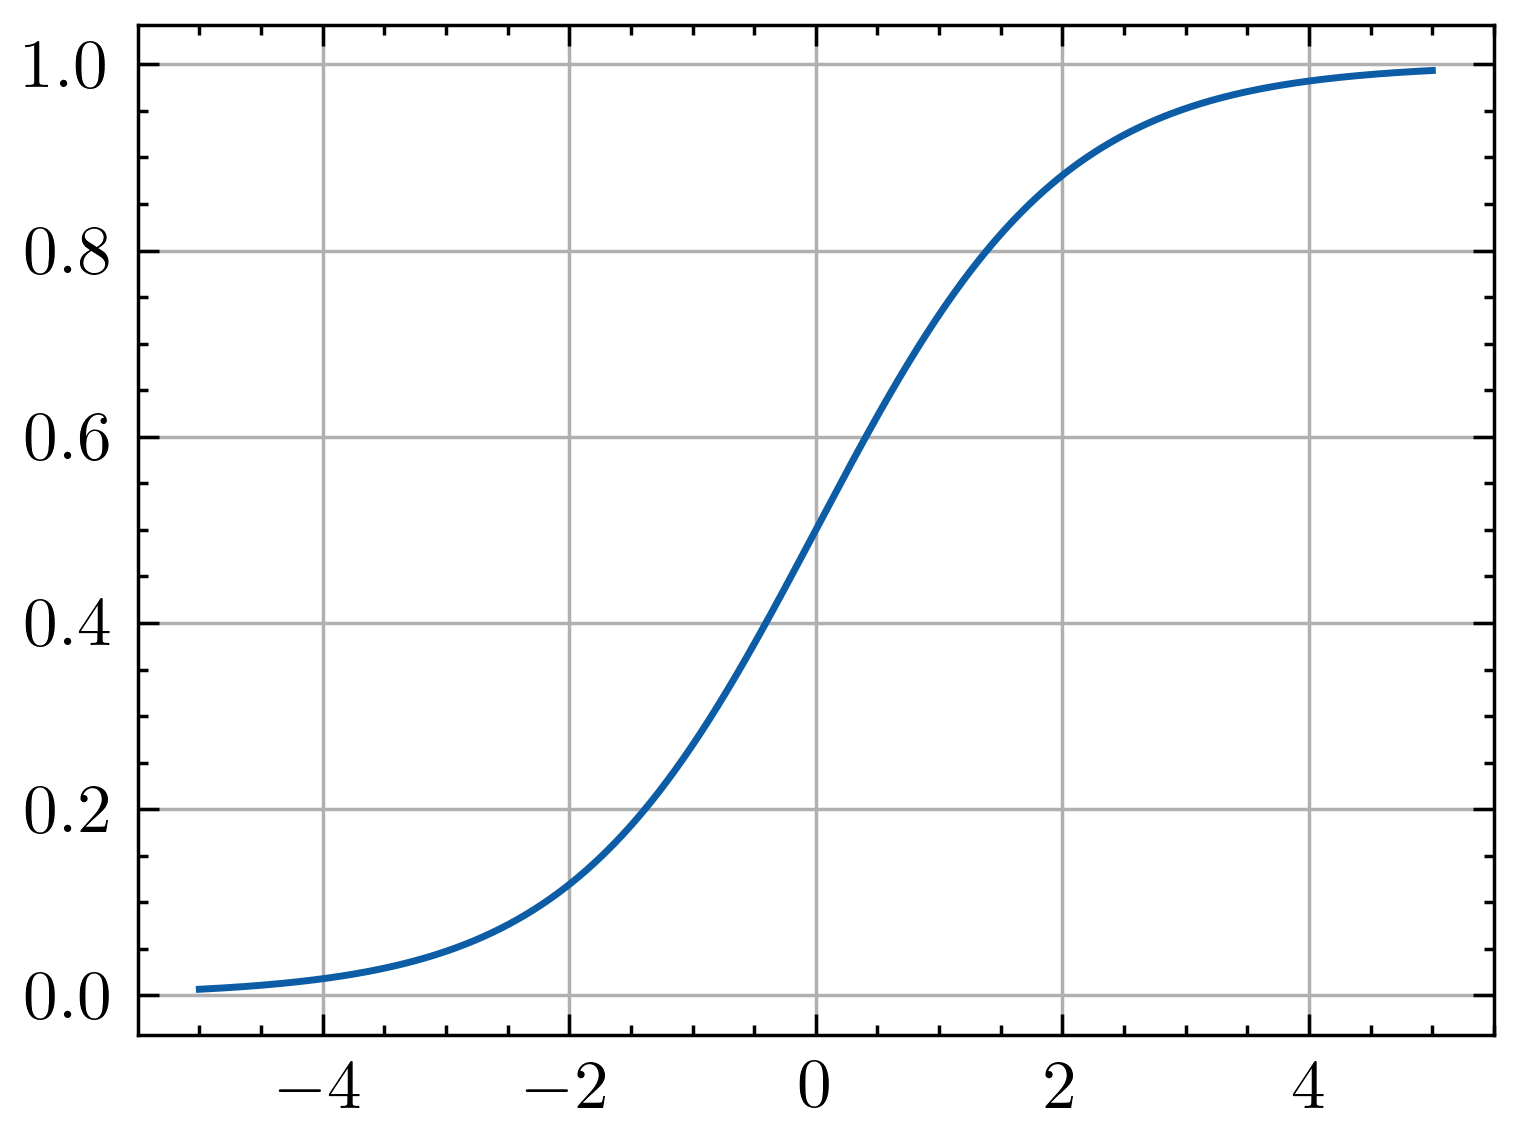
\includegraphics[width=0.8\textwidth]{figuras/sigmoid.png}
    \caption{Gráfica de la función sigmoide. Elaboración propia.}
    \label{fig:sigmoid}
\end{figure}


\paragraph{Unidades Softmax}\mbox{}\\

Cualquier momento que queramos representar una distribución de probabilidad sobre una variable discreta con $n$ valores posibles, usaremos la función \textit{softmax}. Puede ser vista como una generalización de la función sigmoide, que fue usada para representar una distribución de probabilidad sobre una variable binaria.

Para generalizar al caso de una variable discreta con $n$ valores, necesitamos producir un vector $\hat{y}$, con $\hat{y}_i=P(y=i|x)$. No solo necesitamos que cada elementos del vector esté entre 0 y 1, sino que además la suma de todo el vector sea igual a 1. Repitiendo el procedimiento usado para las sigmoides podemos generalizar la distribución. Primero, una capa lineal predice probabilidades logarítmicas no normalizadas:
\begin{equation}
    z = W^Th+b
\end{equation}
donde $z_i = \log \tilde{P}(y=i|x)$. Entonces, la función softmax puede exponenciar y normalizar $z$ para obtener $\hat{y}$. Formalmente, la función softmax está dada por: 
\begin{equation}
    softmax(z)_i=\frac{\exp{(z_i)}}{\sum_j \exp{(z_j)}}
\end{equation}

Al igual que en el caso de la función logística, el uso de la exponencial funciona bien cuando entrenamos el softmax para predecir el valor $y$ usando máxima verosimilitud.

\subsection{Unidades ocultas}
Como hemos mencionado anteriormente, cualquier unidad de salida que hemos explicado también puede ser aplicada como unidad oculta. Aún así, existen otras funciones de activación para este caso. Cabe destacar que la investigación sobre el diseño de las unidades ocultas sigue activo. Nosotros nos centraremos en algunas de las más comunes.

\paragraph{Unidades Lineales Rectificadas (ReLU) y sus generalizaciones}\mbox{}\\
Las unidades lineales rectificadas usan la función de activación $g(z)=\max \{0, z\}$. Son fáciles de optimizar porque son muy parecidas a las unidades lineales. La única diferencia es que estas devuelven cero en la mitad de su dominio. Esto permite que las derivadas mediante una unidad linear rectificada se mantengan grandes siempre que la unidad está activa. Los gradientes además son consistentes. Además, la segunda derivada de una ReLU es 0 casi en todo punto, y la derivada primera es 1 donde la unidad está activa.

\begin{figure}[h]
    \centering
    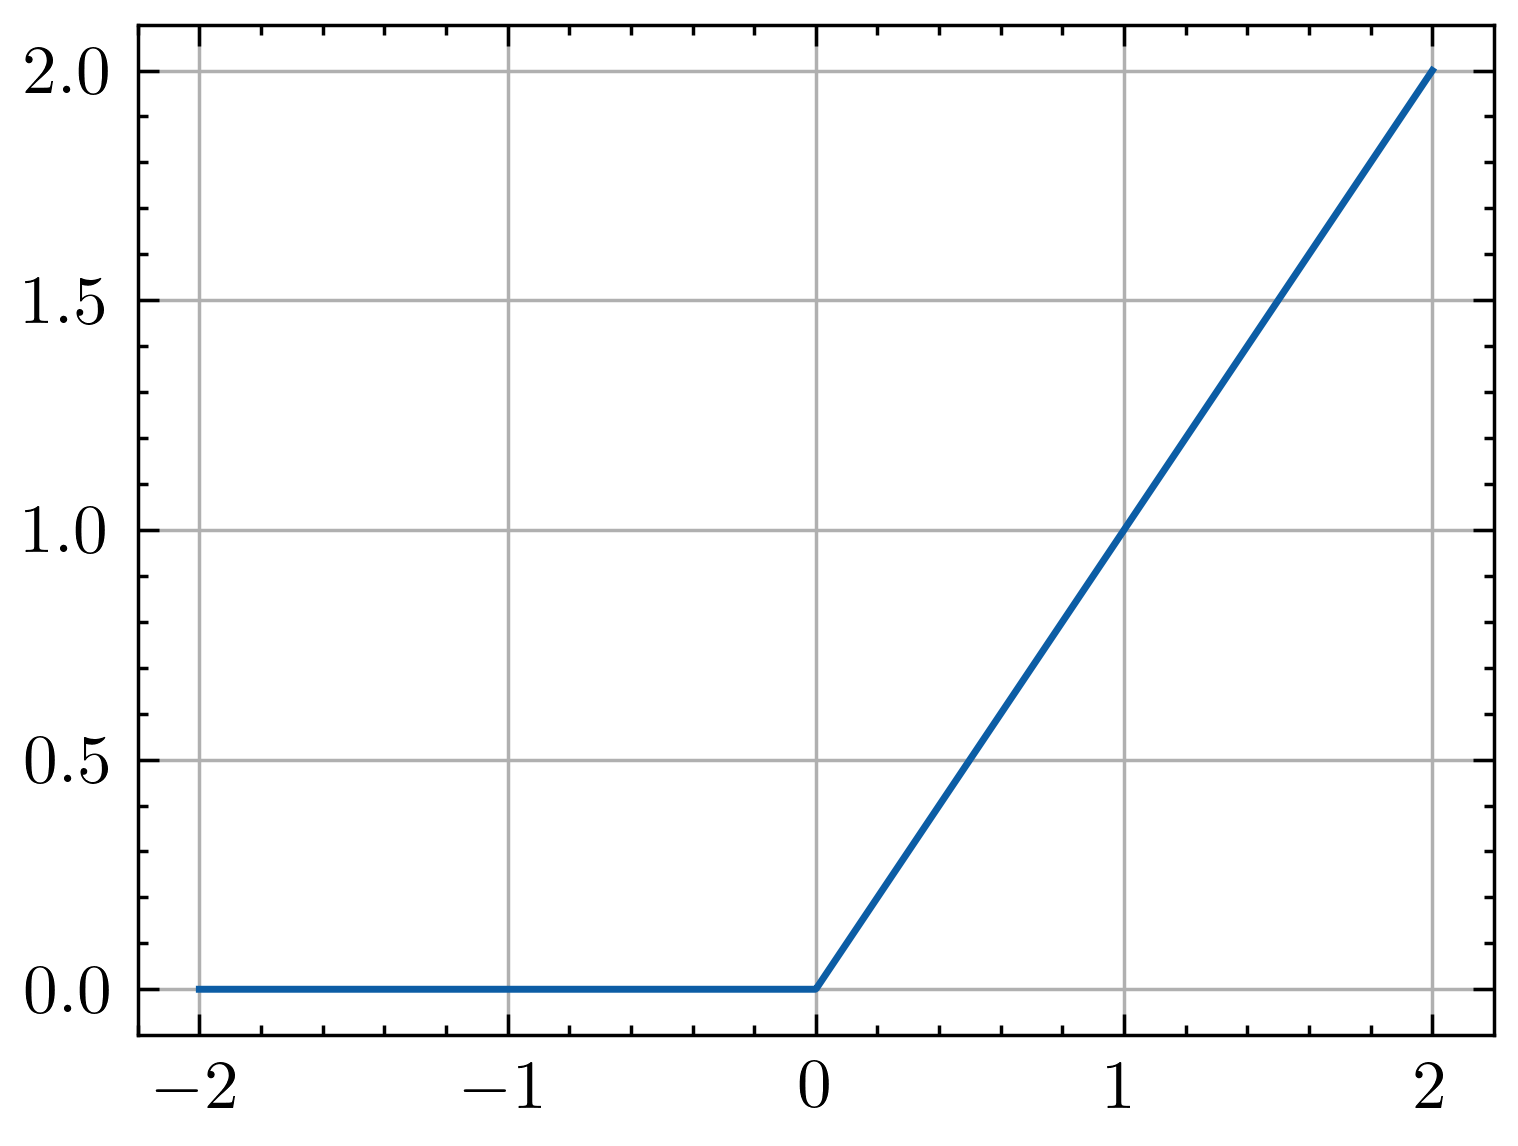
\includegraphics[width=0.8\textwidth]{figuras/relu.png}
    \caption{Gráfica de la función ReLU. Elaboración propia}
    \label{fig:relu}
\end{figure}

Existen bastantes generalizaciones de las ReLU. La mayoría de estas generalizaciones funcionan de manera comparable o incluso mejor que las primeras. Muchas generalizaciones se centran en solventar el problema de que no pueden aprender por descenso por el gradiente cuando su activación es cero.
\begin{itemize}
    \item \textbf{Rectificación de valor absoluto} consiste en fijar una pendiente de -1 cuando la salida de la ReLU es menor que 0, haciendo así $g(z)=|z|$.
    \item \textbf{Leaky ReLU} fija una pendiente muy pequeña como 0.01 cuando la salida de la ReLU es 0.
    \item \textbf{ReLU paramétrica} trata la pendiente ya mencionada como un valor a aprender.
\end{itemize}

\paragraph{Sigmoide Logística y Tangente Hiperbólica}\mbox{}\\
Antes de que se introdujesen las ReLU, la mayoría de redes neuronales usaban la función logística sigmoide como función de activación o la tangente hiperbólica.
\begin{gather}
    g(z) = \frac{1}{1 + e^{-z}} \\
    g(z) = \tanh{(z)}
\end{gather}

Estas funciones están estrechamente relacionadas pues $\tanh{(z)=2\sigma(2z)-1}$.

Ya hemos visto las unidades sigmoide como unidades de salida, usadas para predecir la probabilidad de que una variable binaria tome el valor 1. Sin embargo, las unidades sigmoidales se saturan en la mayor parte de su dominio, y solo son sensibles cuando su entrada es muy cercana a 0. La amplia saturación de las unidades sigmoidales hace que el aprendizaje por el gradiente sea muy difícil y es por ello que no se recomienda su uso como unidades ocultas. Solo se recomiendan cuando tengamos una función de coste capaz de deshacer la saturación de esta.

Las funciones de activación sigmoide son más comunes en otros escenarios que en \ac{MLP}. Las redes recurrentes, muchos modelos probabilísticos, y algunos \textit{autoencoders} tienen requisitos adicionales que hacen el uso de funciones sigmoidales más atractivos pese a la desventaja de la saturación.

\section{Redes Convolucionales}
Una \ac{CNN}~\cite{Goodfellow-et-al-2016} es un tipo especializado de red neuronal para procesar datos que tenga una topología de rejilla. Esto incluye datos en series temporales, que pueden ser pensados como una rejilla 1 dimensional a intervalos de tiempo regulares, e imágenes, que pueden ser pensadas como una rejilla 2 dimensional de píxeles. Las \ac{CNN} han demostrado ser realmente exitosas en múltiples aplicaciones prácticas. El nombre de ``red neuronal convolucional`` indica que la red hace uso de la operación de convolución. 

Vamos a explicar que es la convolución, cuál es la motivación para usarla en una red neuronal, descubriremos la técnica de \textit{pooling} que es usada a día de hoy en la mayoría de las redes convolucionales y nombraremos algunas redes importantes de este tipo.

\subsection{La Operación de Convolución}
En su forma más general, la convolución es una operación que toma como argumento dos funciones de variable real. Sean $f, g: \mathbb{R} \to {R}$ dos funciones de variable real, la convolución de ambas funciones se denota por $(f \star g)$ a su convolución y viene definida por:
\begin{equation}
    s(t) = (f \star g) = \int_{-\infty}^{\infty}f(s)g(t-s)ds
\end{equation}

Si usamos la terminología de las \ac{CNN}, nuestro primer argumento, es decir $f$ se le conoce como la entrada, y al segundo, $g$, será el núcleo o \textit{kernel} de la convolución. Al resultado en ocasiones se le llama mapa de características o \textit{feature map}.

Normalmente, cuando trabajamos con datos en un ordenador, no podemos tratar con un continuo sino con datos discretizados. Por lo tanto asumir que podemos evaluar las funciones en todo punto no es realista. Es por ello que definimos la operación de convolución discreta como será natural viendo la definición anterior:
\begin{equation}
    s(t) = (f \star g) = \sum_{s=-\infty}^{\infty}f(s)g(t-s)
\end{equation}

En el \ac{AA}, las entradas normalmente suelen ser tensores de datos, y el \textit{kernel} suele ser también un \textit{kernel} de parámetros que son adaptados por el algoritmo de aprendizaje que usemos. Debido a que cada elemento de la entrada y del \textit{kernel} debe de ser almacenado por separado, asumimos que estas funciones son cero en todos los puntos salvo en el conjunto finito del que almacenamos valores. En práctica, esto significa que podemos implementar la suma infinita como una suma finita de elementos de los tensores.

Además, también usaremos convoluciones sobre más de un eje a la vez. Por ejemplo, si usamos una imagen de dos dimensiones $I$ como entrada, posiblemente también consideremos usar un \textit{kernel} de dos dimensiones $K$:
\begin{equation}
    S(i,j) = (I \star K)(i,j) = \sum_m \sum_n I(m,n)K(i-m, j-n)
\end{equation}
Además, la convolución también es conmutativa por lo que podemos escribir también:
\begin{equation}
    S(i,j) = (K \star I)(i,j) = \sum_m \sum_n K(m,n)I(i-m, j-n)
\end{equation}
Normalmente se implementa la última fórmula pues hay menos variación en el rango de valores válidos de $m$ y $n$.

\subsection{Motivación}
La convolución implica tres ideas importantes que pueden ayudar a mejorar un sistema de \ac{AA}: compartir parámetros, interacciones dispersas y representaciones equivariantes. Además, también nos permite un método para trabajar con entradas de tamaño variable.

Las capas tradicionales de redes neuronales usan la multiplicación por una matriz de parámetros con un parámetro parámetro separado que describe la interacción entre cada unidad de entrada y cada unidad de salida. Esto significa que cada unidad de salida interacciona con cada unidad de entrada. Sin embargo, una \ac{CNN} suele tener interacciones dispersas. Esto es cuando el \textit{kernel} es más pequeño que la entrada (que suele ser el caso habitual). Por ejemplo, cuando procesamos una imagen, la imagen puede tener miles o millones de píxeles, pero podemos detectar características pequeñas pero útiles tales como bordes con \textit{kernels} que son del tamaño de cien píxeles o menos. Esto significa que necesitamos almacenar menos parámetros, lo que reduce requisitos de memoria y mejora la eficiencia estadística del modelo. También implica que calcular el resultado del modelo necesita de menos operaciones. Estas mejoras en eficiencia suelen ser bastantes grandes. Si hay $m$ entradas y $n$ salidas, entonces la multiplicación de matrices necesita de $m \times n$ parámetros y los algoritmos tendrán una complejidad de $O(m \times n)$. Si limitamos el número de conexiones con cada salida a $k$, entonces solo necesitaremos $k \times n$ parámetros. Para muchas aplicaciones prácticas, es posible obtener un buen rendimiento en la tarea de \ac{AA} mientras mantenemos $k$ órdenes de magnitud por debajo de $m$.

Compartir parámetros se refiere al uso de un mismo parámetro para más de una función en un modelo. En las arquitecturas tradicionales de redes neuronales, cada elemento de la matriz de pesos se usa exactamente una vez cuando se calcula la salida de una capa. En una \ac{CNN}, cada elemento del \textit{kernel} se usa en cada posición de la entrada (excepto quizás en el borde de esta). Que se compartan los parámetros significa que en lugar de aprender un parámetro para cada ubicación de la entrada se aprende únicamente un conjunto de ellos. Esto no afecta al tiempo de ejecución de un paso de la red, pero si disminuye los requisitos de memoria del modelo. Por lo tanto, las convoluciones son dramáticamente más eficaces que las matrices densas en términos de memoria y eficiencia estadística.

En el caso de la convolución, el hecho de compartir parámetros implica que la capa tiene una propiedad llamada equivarianza a translaciones. Decir que una función es equivariante significa que si la entrada cambia, la salida se mantiene igual. Formalmente, una función $f(x)$ es equivariante a una función $g$ si $f(g(x))=g(f(x))$. En el caso de la convolución, si $g$ es cualquier translación, esto es, desplaza la entrada, entonces la convolución es invariante a $g$. En el caso de imágenes, la convolución crea un mapa 2-D de dónde aparecen ciertas características en la entrada. Por ejemplo, es útil detectar bordes en la primera capa de una \ac{CNN}. Los bordes aparecen más o menos en todas las partes de la imagen, así que tiene sentido compartir los parámetros para toda la imagen. En algunos casos, si estamos procesando imágenes recortadas para estar centradas respecto a algo, como por ejemplo, la cara de una persona, tal vez no nos interese compartir parámetros.


\subsection{Pooling}

Una capa de una \textit{CNN} suele estar formada por tres etapas. En la primera etapa, la capa realiza convoluciones en paralelo para producir un conjunto de activaciones lineales. En la segunda etapa, cada activación lineal se ejecuta con una función de activación no lineal, tales como ReLU. En la tercera etapa, usamos una función de \textit{pooling} para modificar la salida de la capa.

Una función de \textit{pooling} reemplaza la salida de la red en una cierta localización con un estadístico de las salidas cercanas. Por ejemplo, el \textit{max pooling} consiste en calcular la salida máxima dentro de un entorno rectangular. Otras funciones de \textit{pooling} populares son calcular el promedio en un entorno rectangular, la norma $L^2$ de un entorno rectangular o la media ponderada basada en la distancia del píxel central.

En todos los casos, el \textit{pooling} nos ayuda a hacer una representación aproximadamente invariante a pequeñas translaciones de la entrada. La invariancia a translaciones locales puede ser una propiedad útil si nos interesa más la presencia de algunas características que el saber exactamente dónde están. Por ejemplo, para determinar si una imagen contiene un rostro, no necesitamos saber la posición de los ojos con una precisión perfecta, solo saber que hay un ojo izquierdo a la izquierda de la cara y un ojo derecho a la derecha de la cara.

Para muchas tareas, el \textit{pooling} es esencial para manejar entradas de tamaño variable. Por ejemplo, si queremos clasificar imágenes de un tamaño variable, la entrada a la capa de clasificación debe de tener un tamaño fijo. Esto normalmente se logra adaptando el tamaño de las regiones de \textit{pooling} de manera que la capa de clasificación siempre reciba el mismo número de características sin importar el tamaño de la entrada. Por ejemplo, la última capa de \textit{pooling} en una red puede estar definida para dar siempre cuatro características, una por cada cuadrante de la imagen, sin importar el tamaño de esta.

\section{EfficientNet}

Durante el desarrollo de este trabajo haremos uso de la arquitectura de \textit{EfficientNet}~\cite{efficientnet}. Esta arquitectura es un tipo de red convolucional centrada en escalar apropiadamente la profundidad, anchura y resolución de la red con el fin de obtener un mejor rendimiento.

\subsection{Escalado del modelo}
El problema que intenta resolver \textit{EfficientNet} es encontrar un buen factor de escalado entre la anchura, profundidad y resolución de la red. Para ello, primero se debe de formular el problema de forma teórica.

La capa $i$ de una red convolucional se puede definir como una función $Y_i=\mathcal{F}_i(X_i)$, donde $\mathcal{F}_i$ es el operador, $Y_i$ es el tensor de salida y $X_i$ es el tensor de entrada con forma $(H_i, W_i, C_i)$, donde $H_i$ y $W_i$ son las dimensiones espaciales y $C_i$ es la dimensión de los canales de la imagen. Una red convolucional se puede representar como una lista de capas compuestas: $\mathcal{N}=\mathcal{F}_k \circ \ldots \circ \mathcal{F}_2 \circ \mathcal{F}_1(X_1)$. En la práctica, muchas redes convoluciones se dividen en etapas y todas las capas en la misma etapa comparten la misma arquitectura. Por lo tanto se puede definir una red convolucional como:
\begin{equation}
    \mathcal{N}=\circ_{i=1,\ldots,s}F_i^{L^i}(X_{(H_i, W_i, C_i)})
\end{equation}

donde $F_i^{L_i}$ denota que la capa $F_i$ se repite $L_i$ veces en la etapa $i$. 

El objetivo de\textit{ EfficientNet}~\cite{efficientnet} consiste en expandir la longitud ($L_i$), anchura ($C_i$) y/o resolución ($H_i, W_i$) sin cambiar $\mathcal{F}_i$, la cual ya está previamente definida por una arquitectura base. Esto simplifica el problema de diseño pero sigue dejando un amplio espacio para explorar distintos parámetros para cada capa. Con el fin de reducir este espacio, los autores deciden restringir a que todas las capas deben de ser escaladas de manera uniforme con un ratio constante.

Los autores observan de manera empírica que las diferentes dimensiones en las que escalar no son independientes. Intuitivamente, para imágenes de mayor resolución, se debe de aumentar la profundidad de la red, con el fin de que campos receptores más grandes puedan ayudar a capturar características similares que incluyen más píxeles en imágenes más grandes. A su vez, también se debería de aumentar la anchura de la red cuando la resolución es mayor, con el objetivo de capturar patrones más finos con más píxeles. Por lo tanto se necesita coordinar y equilibrar las dimensiones sobre las que escalamos en lugar de escalar una única dimensión.

\subsection{La Arquitectura de EfficientNet}
Una vez dada la técnica de escalado para una red base, queda clara la importancia de esta última. Para obtener una arquitectura nueva, los autores han usado una búsqueda multi-objetivo de redes neuronales que optimiza tanto los \textit{FLOPS} como la precisión. Concretamente usando como función a optimizar $ACC(m)\times [FLOPS(m)/T]^\omega$ donde $ACC(m)$ es la precisión del modelo m, $FLOPS(m)$ los \textit{FLOPS} del modelo, $T$ el objetivo de \textit{FLOPS} a conseguir y $\omega=-0.007$ un hiperparámetro para compensar entre la precisión y los $FLOPS$. El resultado de esta búsqueda es un modelo llamado \texttt{EfficientNet-B0}. Aplicando posteriormente la técnica de escalado logran crear los modelos \texttt{EfficientNet-B1} hasta \texttt{EfficientNet-B7} siendo este último un modelo estado del arte en el momento de publicación de \cite{efficientnet}, siendo 8.4 veces más pequeña y 6.1 veces más rápida que la mejor red convolucional existente previamente.
 

\part{Preliminares en Aprendizaje Federado y Blockchain}\label{sec:fundamentosAaBl}
\chapter{Federated Learning}\label{sec:fl}
\section{Introducción}
El \textit{deep learning} ha revolucionado el campo de la \ac{IA} mediante la posibilidad de permitir a las máquinas a aprender y tomar decisiones como los humanos gracias a técnicas basadas en datos. El de desarrollo en redes de alta velocidad tales como 5G y avances en \textit{edge computing} ha permitido el desarrollo de modelos y hardware capaces de procesar grandes cantidades de datos recolectados de múltiples dispositivos. En consecuencia, la privacidad se ha convertido en una gran influencia en el diseño, llevando los esfuerzos desde el \ac{AA} centralizado al \ac{AA} distribuido. Aún así, en el \ac{AA} distribuido los costes de comunicación son inmensamente mayores que los costes de cómputo, haciendo el proceso de entrenamiento ineficiente. El \ac{FL} o \textit{Federated Learning} fue inventado para resolver estos problemas~\cite{tutorial-nuria}. En esencia, \ac{FL} es un paradigma de aprendizaje distribuido que permite a un modelo aprender a partir de datos distribuidos, sin la necesidad de estos de ser recolectados por un servidor central. Dado que los dados locales nunca abandonan los dispositivos donde son recogidos, se garantiza la privacidad de datos.

\ac{FL} ha ganado atención debido a su capacidad de resolver preocupaciones sobre la privacidad y de mejorar la eficiencia de aprendizaje distribuido. Además, es altamente escalable ya que puede soportar una gran cantidad de participantes, cada uno con su respectivas fuentes de datos. Esto puede ser realmente útil en escenarios con una generación continua de datos como puede ser el \ac{IoT}, sensores, etc. Como resultado, \ac{FL} se ha convertido en un campo importante de la \ac{IA} obteniendo el interés de investigadores, desarrolladores y científicos de datos en la comunidad del \ac{AA}. El primer caso de uso exitoso del \ac{FL} fue desarrollado por Google~\cite{mcmahan-2018} para predecir la siguiente entrada de texto del usuario en miles de dispositivos Android, mientras se mantenía los datos de los dispositivos en local. Desde entonces, el \ac{FL} se ha aplicado a un gran rango de aplicaciones en diversos campos, desde ingeniería industrial hasta el mundo de la salud~\cite{survey-nuria-2023}. 

\section{Federated Learning: ¿Qué y Por Qué?}
El \ac{AA} basado en datos domina actualmente el campo de la \ac{IA}. Desafortunadamente, la creciente demanda en término de volumen de datos y variedad ha resultado en varios problemas relacionado en la privacidad de los datos y en el procesamiento de grandes cantidades de datos. Entre ellos, los principales desafíos del \ac{AA} que llevan a la aparición del \ac{FL} están asociados con la privacidad, comunicación y acceso a los datos~\cite{tutorial-nuria}.

\begin{itemize}
    \item \textbf{Privacidad de los Datos}: en el \ac{AA} centralizado, los datos de los usuarios son recolectados y se almacenan en un servidor central, donde pueden ser vulnerables a una brecha de seguridad. Además, la creciente preocupación sobre la protección de los datos se manifiesta en el área legal. Por lo tanto, hay una urgente demanda en el desarrollo de métodos de \ac{IA} que protejan la privacidad.

    \item \textbf{Costes de Comunicación y Latencia}: en el \ac{AA} centralizado, los datos sin procesar son mandados al servidor central para ser procesados y usados para entrenar el modelo. Este intercambio de información puede ser costoso, especialmente cuando se trata con conjuntos de datos muy grandes. Además, la creciente cantidad de datos disponibles debido al drástico aumento de sensores \ac{IoT} y dispositivos móviles generando enormes cantidades de datos supone un nuevo desafío relacionado con el almacenamiento y preprocesamiento de un flujo continuo de datos.

    \item \textbf{Limitaciones al Acceso de Datos}: en algunos casos, los datos pueden ser distribuidos entre diferentes instituciones u organizaciones, haciendo complicado el acceder o compartir datos entre ellas.
\end{itemize}

Con el objetivo de resolver los desafíos previamente mencionados, \ac{FL} aparece como un paradigma de \ac{AA} distribuido enfocado en desarrollar un modelo de \ac{AA} sin explícitamente compartir ningún dato entre los participantes. Implica una red de clientes $\{C_1, C_2, \ldots, C_n \}$, que participa en dos fases principales:

\begin{enumerate}
    \item \textbf{Fase de Entrenamiento del Modelo}: cada cliente (o propietario de datos) intercambia información sin revelar ningún dato de su conjunto para entrenar de forma conjunta un modelo de \ac{AA}. Para lograr esto, cada cliente entrena un modelo local con sus datos y comparte la información de este modelo en lugar de sus datos de entrenamiento. Entonces, los modelos locales son agregados para crear un modelo global.
    \item \textbf{Fase de Inferencia}: el modelo global es aplicado a nuevas instancias de datos.
\end{enumerate}

Estos procesos pueden ser tanto síncronos como asíncronos dependiendo de la disponibilidad de los nodos y del modelo entrenado. Es importante notar que la privacidad no es la única razón para aplicar este método, ya que también se debería usar alguna estrategia para compartir los beneficios del modelo entrenado de forma colaborativa.

Una vez hemos descrito \ac{FL} como un concepto general, un escenario de \ac{FL} puede ser propuesto formalmente de la siguiente manera. Suponemos un conjunto de clientes $\{C_1, \ldots, C_n\}$ con sus respectivos conjuntos de datos de entrenamiento $\{D_1, \ldots, D_n\}$. Cada uno de estos clientes $C_i$ cuenta un con modelo local $L_i$ expresado como los parámetros $\{L_1, \ldots, L_n\}$. El \ac{FL} se enfoca en aprender un modelo global $G$, usando datos distribuidos entre clientes mediante un proceso de aprendizaje iterativo conocido como \textbf{ronda de aprendizaje}. Para ello, en cada ronda de aprendizaje $t$, cada cliente entrena su modelo local sobre sus datos locales $D_i^t$, resultando en la actualización de los parámetros locales $L_i^t$ a $\hat{L}_i^t$. Después, los parámetros globales $G^t$ son calculados agregando los parámetros locales entrenados $\{\hat{L}_1^t, \ldots, \hat{L}_n^t\}$ usando una operación fija de agregación denotada por $\Delta$. Luego los parámetros locales son actualizados con los parámetros globales agregados.
\begin{equation}
    G^t = \Delta (\hat{L}_1^t, \ldots, \hat{L}_n^t)
\end{equation}
\begin{equation}
    L^{t+1}_i \leftarrow G^t, \quad \forall i \in \{1, \ldots, n\}.
\end{equation}

Las actualizaciones entre los clientes y el servidor son repetidas durante el proceso de aprendizaje hasta que se alcanza algún criterio de parada. Así, el valor final de $G$ resumirá el conocimiento modelado en los clientes.

\section{Elementos Clave en Federated Learning}
Una vez que el \ac{FL} ha sido introducido de manera breve, podemos hablar del flujo de trabajo de un proceso de \ac{FL}. Este se compone de los siguientes pasos:
\begin{enumerate}
    \item \textbf{Entrenamiento local}: comienza con el entrenamiento local de cada uno de los modelos locales por cada uno de los clientes. Generalmente, todos estos modelos tienen una arquitectura común. Sin embargo, los aspectos relacionados con los hiperparámetros de entrenamiento (\textit{epochs}, \textit{batch size}, \textit{learning rate}) puede diferir entre clientes. En esta fase los primeros elementos aparecen de manera natural:
    \begin{itemize}
        \item \textbf{Datos Descentralizados}: los datos se encuentran distribuidos entre los distintos dispositivos o nodos, en lugar de en un mismo lugar de forma centralizada, lo cual es un beneficio cuando la privacidad es una preocupación. La distribución de los datos puede ser:
        \begin{enumerate}
            \item \textbf{Homogénea o \ac{i.i.d.}}: se asume que la distribución de datos entre los clientes es \ac{i.i.d.}, por lo que todos los clientes tienen la misma distribución.
            \item \textbf{Heterogénea o no-i.i.d.}: se asume que la distribución de datos entre los clientes no es \ac{i.i.d.}, esto es, que los datos de cada cliente sigue una distribución distinta. Formalmente se pueden distinguir entre tres tipos de heterogeneidad de la distribución de datos:
            \begin{itemize}
                \item El espacio de características de nuestros clientes es distinto pero comparten el mismo objetivo.
                \item El espacio de entradas es análogo pero el espacio de las etiquetas es distintos respecto a los mismos datos.
                \item Ambos espacios son distintos.
            \end{itemize}
        \end{enumerate}

        \item \textbf{Modelo}: el entrenamiento del modelo es realizado en los datos descentralizados, donde cada dispositivo o nodo entrena su modelo y contribuye al proceso de entrenamiento, compartiendo los pesos de su modelo local. También mejora el modelo debido a una mejor generalización, ya que el modelo puede aprender de un rango más amplio de datos.
        \item \textbf{Clientes}: estos nodos almacenan datos y entrenan modelos locales.
    \end{itemize}
    
    \item \textbf{Comunicación}: después del entrenamiento local, la comunicación permite la coordinación y agregación de las actualizaciones del modelo generadas por los participantes, permitiendo así un entrenamiento distribuido. Es un rol crucial en la protección de la privacidad y seguridad de los datos cuando se combina con varias técnicas como la \ac{DP}. Destacamos los siguientes elementos clave en este paso:
    \begin{itemize}
        \item \textbf{Planificación de Comunicaciones}: la comunicación puede ser tanto síncrona como asíncrona, dependiendo de la configuración. También puede haber un servidor central que maneja la recolección de todos los modelos locales, o puede estar distribuido a través de múltiples nodos en la red.

        \item \textbf{Protocolos de Privacidad}: pese a que no se comparten los datos de entrenamiento durante las comunicaciones en \ac{FL}, la información compartida es susceptible a brechas de privacidad o a corromper el proceso de aprendizaje en su totalidad. Por lo tanto, las comunicaciones son uno de los puntos débiles de \ac{FL} respecto a los ataques. Por esta razón es normal combinarlas con otros mecanismos de privacidad.
    \end{itemize}

    \item \textbf{Agregación}: las actualizaciones locales generadas por cada nodo son combinadas mediante un operador específico de agregación y el resultado es incorporado para actualizar y crear un modelo global entrenado. El elemento clave en este paso es el \textbf{mecanismo de agregación}, que depende en la tarea que se plantea resolver. Pese a ello, el mas común es \textbf{\ac{FedAvg}} cuando el modelo se puede expresar como un vector de pesos. En otro caso, como podría ser el \textit{clustering}, se debe de diseñar un agregador específico para combinar la información de cada nodo.
    \item \textbf{Actualización local}: el último paso consiste en actualizar los modelos locales almacenados en los distintos nodos con el nuevo modelo global. El caso más sencillo es actualizar todos los modelos locales con el modelo global. Sin embargo, hay distintas estrategias de actualización que consisten en en combinar el modelo local y el global en lugar de reemplazar el uno por el otro directamente. Estos enfoques son usados para alcanzar características tales como la personalización de los clientes a sus datos locales.
\end{enumerate}

\section{Arquitecturas de Federated Learning}
La combinación de los elementos clave genera muchas arquitecturas de \ac{FL} que definen su interrelación, ambas cliente-servidor y \textit{peer-to-peer}:
\begin{itemize}
    \item \textbf{Arquitectura Cliente-servidor}: hay un nodo que es el responsable de la coordinación y agregación de las actualizaciones del modelo que recibe el nombre de \textbf{servidor} y el resto de nodos responsables del entrenamiento de los datos locales con sus propios datos son llamados \textbf{clientes}. Es fácil de implementar pero requiere un nivel de confianza elevado en el servidor. Este grado de confianza es su principal debilidad y es por ello que es vulnerable a ataques.

    \begin{figure}[h!]
      \centering
      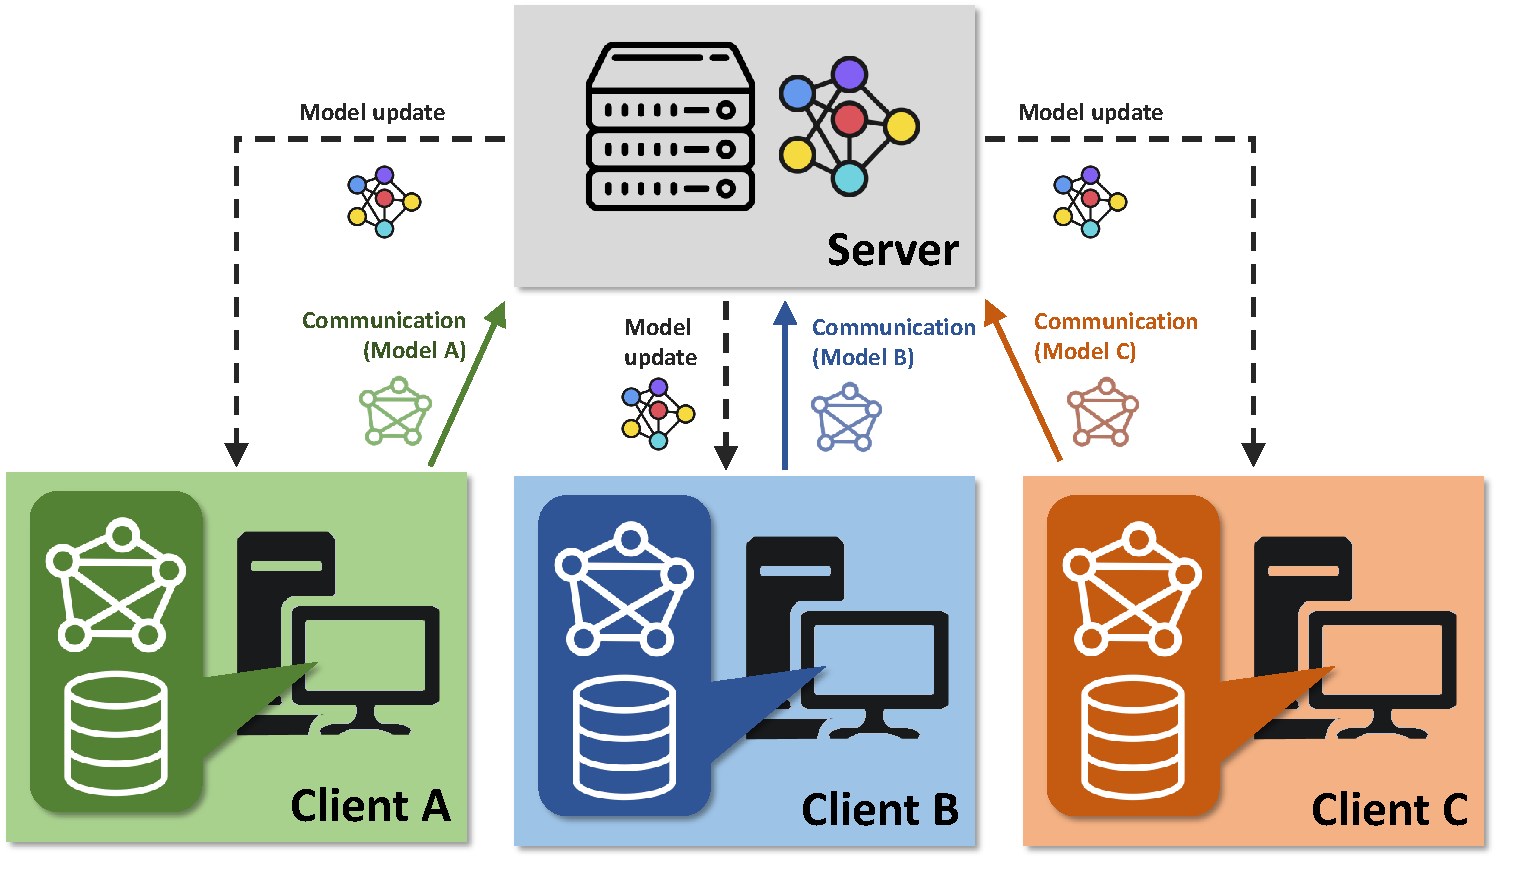
\includegraphics[width = \linewidth]{figuras/cliente-servidor.pdf}
      \caption{Representación de la arquitectura cliente-servidor en \ac{FL} con 3 clientes. Fuente: \cite{tutorial-nuria}.}
      \label{clientserver}
    \end{figure}

    \item \textbf{Arquitectura \textit{Peer-to-peer}}: todos los nodos tienen datos locales de entrenamiento y agregan las actualizaciones de los demás nodos simultáneamente. No necesita de ningún nodo coordinador del proceso de aprendizaje fijo. Es complicada de implementar, y acarrea un aumento en los costes de comunicación, pero la principal ventaja es el elevado nivel de seguridad y privacidad de datos.
\end{itemize}

La arquitectura Cliente-Servidor es la más común en \ac{FL} y consecuentemente nos referiremos a ella como la arquitectura por defecto cuando hablemos de \ac{FL}.

\section{Categorías de Federated Learning}
Hay múltiples categorías de \ac{FL} según las propiedades de los elementos clave~\cite{survey-nuria-2023}. Las siguientes categorías están hechas en términos del espacio de características ($X$), el espacio de etiquetas ($Y$) y el espacio muestral ($I$).
\begin{itemize}
    \item \textbf{\ac{HFL}}: cuando los datos forman una partición entre los clientes basado en las muestras, que significa que cada cliente es propietario de diferentes muestras de el conjunto de entrenamiento general. Formalmente, lo podemos expresar como:
    \begin{equation}
        X_i = X_j, Y_i = Y_j, I_i \ne I_j, \quad \forall D_i, D_j, i \ne j
    \end{equation}
    donde los espacios de características y etiquetas de los clientes ($i, j$) están representados por ($X_i, Y_i$) y ($X_j, Y_j$) y asumiendo que son iguales, mientras que las muestras $I_i$ y $I_j$ no coinciden. $D_i$ y $D_j$ representan los datos de los clientes $i$ y $j$. Es adecuado para entrenar modelos en datos recolectados por una gran cantidad de dispositivos similares, tales como \textit{smartphones} o dispositivos \ac{IoT}.
    \item \textbf{\ac{VFL}}: cuando los datos forman una partición entre los clientes basado en las características, lo que significa que cda cliente es propietario del mismo conjunto de muestras pero con un conjunto de características distinto. Formalmente, lo podemos expresar como:
    \begin{equation}
        X_i \ne X_j, Y_i \ne Y_j, I_i = I_j, \quad \forall D_i, D_j, i \ne j
    \end{equation}
    Es adecuado para entrenar modelos en datos recolectados por una cantidad pequeña de dispositivos con un espacio de características distinto. Por ejemplo, puede ser usado para predecir resultados médicos basado en los datos recolectados por múltiples hospitales, donde cada hospital tiene un conjunto distinto de registros.
    \item \textbf{\ac{FTL}}: cuando se transfiere conocimiento entre múltiples dominios sin que haya solapamiento entre muestras o características. Formalmente, lo podemos definir como: 
    \begin{equation}
        X_i \ne X_j, Y_i \ne Y_j, I_i \ne I_j, \quad \forall D_i, D_j, i \ne j
    \end{equation}
    En esta arquitectura, no se asume que la distribución de los datos tanto de entrenamiento como de validación sean los mismos y están definidos en el mismo espacio de características. Normalmente es usado en combinación con técnicas de \textit{fine-tuning} con modelos entrenados sobre grandes conjuntos de datos centralizados.
    \begin{figure}[h!]
        \centering
        \begin{subfigure}[]{0.3\textwidth}
            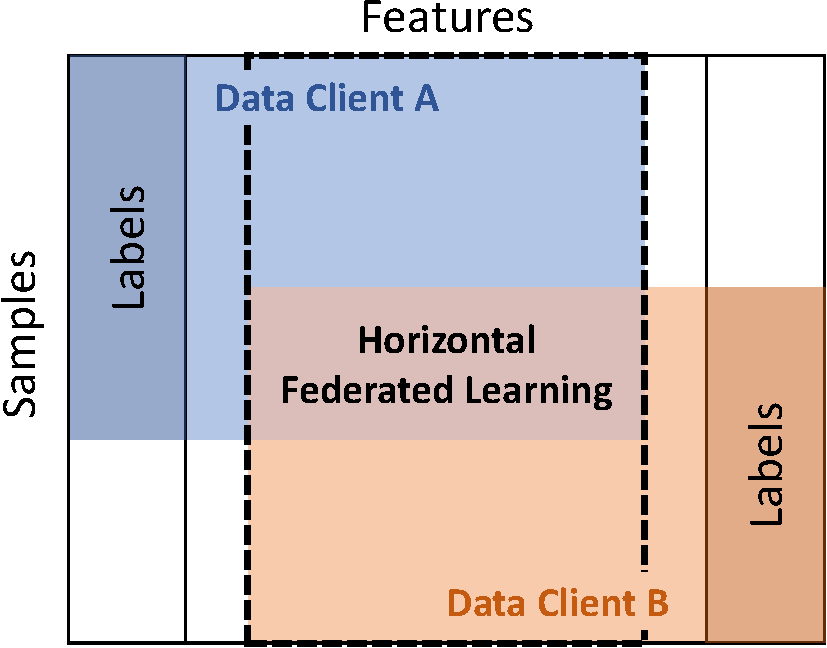
\includegraphics[width=0.95\linewidth]{figuras/hfl.pdf}
            \caption{\ac{HFL} }
            \label{fig:first}
        \end{subfigure}
        
        \hfill
        \vspace{3mm}
        
        \begin{subfigure}[]{0.3\textwidth}
            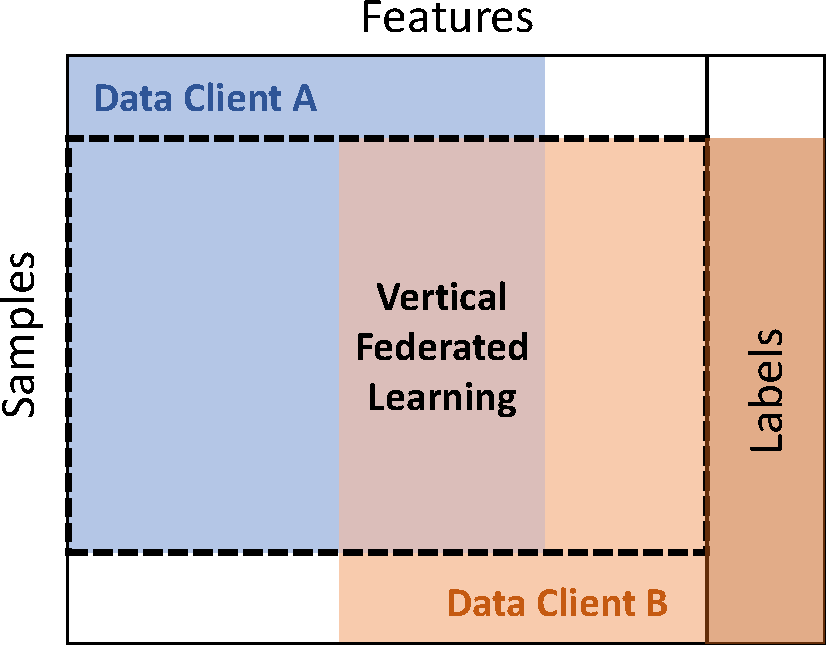
\includegraphics[width=0.95\linewidth]{figuras/vfl.pdf}
            \caption{\ac{VFL} }
            \label{fig:second}
        \end{subfigure}
        
        \hfill
        \vspace{3mm}
        
        \begin{subfigure}[]{0.3\textwidth}
            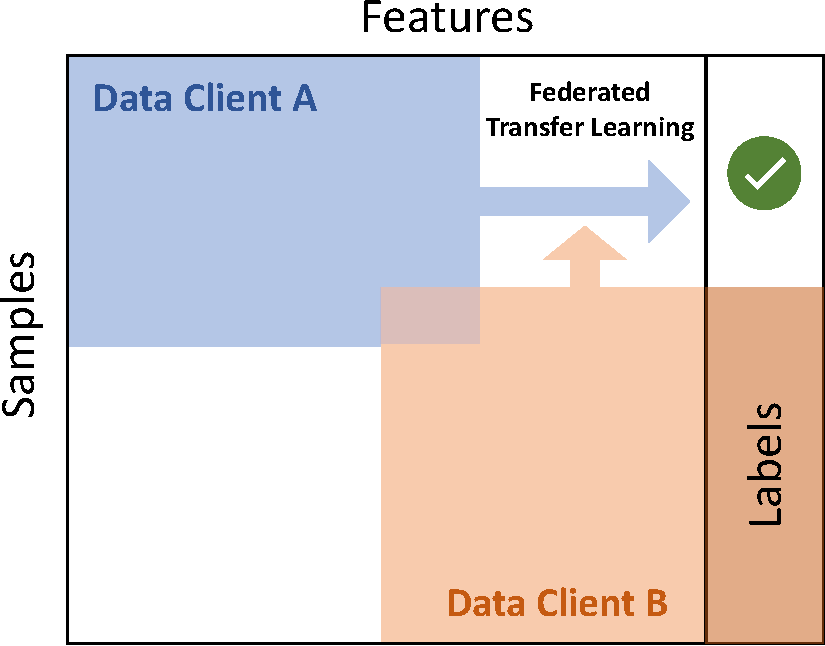
\includegraphics[width=0.95\linewidth]{figuras/ftl.pdf}
            \caption{\ac{FTL}}
            \label{fig:third}
        \end{subfigure}
        \caption{Representación de \ac{HFL}, \ac{VFL} y \ac{FTL} en una arquitectura cliente servidor en \ac{FL} \cite{yang-2019}.}
        \label{fig:architectures}
    \end{figure}

    \section{Privacidad de Datos: técnicas Avanzadas}
    El \ac{FL} ha sido desarrollado teniendo en cuenta la privacidad, esto es, los datos de los clientes se mantiene privado durante el entrenamiento del modelo. Sin embargo, es posible vulnerar estas garantías de privacidad mediante los modelos intercambiados durante el proceso de aprendizaje, ya que los modelos locales de los clientes tienden a memorizar su conjunto de entrenamiento. Un nodo malicioso puede intentar recuperar parte del conjunto de entrenamiento de otros clientes, creando así una brecha de privacidad. Es por ello, se requieren técnicas de privacidad de datos para mejorar las promesas de privacidad de un modelo de \ac{FL}. Consideramos que estas técnicas pueden ser desplegadas en múltiples elementos de la arquitectura de \ac{FL}.
    \begin{enumerate}
        \item \textbf{Computación Segura y Cifrado Homomórfico:} la  computación segura (\textit{Secure Multiparty Computation}) se concentra en asegurar comunicaciones en las rondas de \ac{FL}, principalmente en el mecanismo de agregación. Los canales de comunicación se mantienen seguros mediante el uso de cifrado homomórfico. Mientras estas técnicas evitan interferencias tanto internas como externas durante las rondas de \ac{FL}, el modelo resultante sigue siendo vulnerable a ataques que se enfoquen en extraer información a partir del modelo agregado.
        \item \textbf{Privacidad Diferencial:} la \ac{DP} es una técnica que busca mejorar la privacidad. Se enfoca en ocultar la presencia de los individuos en el modelo. Esto se logra mediante la agregación calibrada de ruido aleatorio. Cuando se aplica en \ac{FL}, la \ac{DP} se puede usar en dos momentos distintos: a) aplicar la \ac{DP} cuando se entrena el modelo localmente (\ac{DP} local), y b) en el paso de agregación creando así una versión diferencialmente privada de \ac{FedAvg}.
    \end{enumerate}

    \section{Ataques a Federated Learning}\label{sec:ataquesfl}
    El \ac{AA} es vulnerable a ataques adversarios enfocados a reducir el rendimiento del modelo o a comprometer la privacidad de datos. Así mismo, el \ac{FL} está igualmente expuesto dado que es un escenario específico de \ac{AA}~\cite{survey-nuria-2023}. Algunos de esos ataques están basados en la manipulación maliciosa de los datos de entrenamiento, que son inaccesibles en el \ac{FL}, y por lo tanto, no podemos confiar en el uso de técnicas de inspección de datos para detectar aquellos datos alterados. Es por ello que, uno de los grandes puntos débiles del \ac{FL} es el ser vulnerable a ataques adversarios que pueden comprometer la integridad del modelo de aprendizaje o la privacidad de los datos.

    Es por esto que esta sección se centrará en dar una serie de taxonomías en ataques de adversarios sobre el \ac{FL}.

    \subsection{Escenarios del Ataque}
    Los escenarios del ataque en \ac{AA} son una representación estructurada de la información, tales que permiten identificar y definir potenciales problemas de seguridad. Pueden ser definidos en términos de la información disponible y en el rango de acción del atacante. En este contexto, definimos los siguientes conjuntos de términos mutuamente exclusivos que nos permiten definir un modelo de ataque en \ac{FL}.

        \paragraph{Atacante externo vs. Interno:} uno de los elementos clave de cualquier sistema distribuido es la comunicación entre distintas partes. La comunicación es muy vulnerable, ya que puede ser comprometida por agentes externos al sistema de aprendizaje, que son conocidos como atacantes externos o \textit{outsiders}. Cuando el ataque es realizado por uno de los participantes del sistema distribuido, ya sea uno o más clientes, o incluso el servidor, se conoce como atacante interno o \textit{insider}. Claramente, el alcance de los dos ataques es bastante diferente. Los ataques internos son son más dañinos y pueden estar enfocados a modificar el comportamiento del modelo o a inferir información de otros clientes, mientras que los ataques externos normalmente solo se enfocan a inferir información sobre los datos o del modelo resultante. Nos enfocamos en los ataques internos, de los que podemos destacar las siguientes categorías:
        \begin{itemize}
            \item \textbf{Ataques Bizantinos}: consisten en mandar actualizaciones arbitrarias al servidor, comprometiendo el rendimiento del modelo global.
            \item \textbf{Ataques sibilino}: consisten en ataques colaborativos, ya sea mediante la agrupación de varios ataques o simulando clientes ficticios con el fin de ser más dañinos.
        \end{itemize}
        
        \paragraph{Cliente vs. Servidor:} respecto a los ataques internos, en el \ac{HFL} es normal diferenciar entre dos tipos de ataques, dependiendo si se están llevando a cabo por un cliente o por un servidor. La principal diferencia recae en la cantidad de información disponible. Mientras que los ataques realizados por clientes solo tienen información de uno o varios clientes, el servidor tiene información sobre la arquitectura del modelo y las actualizaciones de los clientes en cada ronda de aprendizaje. Incluso, en implementaciones criptográficas del medio de comunicación entre clientes y servidor, el servidor tiene más información que los clientes, ya que es el único con suficiente conocimiento para descifrar los modelos.
        
        \paragraph{Conocimiento del Atacante:} en escenarios centralizados, el atacante de caja blanca tiene acceso completo al modelo objetivo, incluyendo su arquitectura, los parámetros y el estado interno. Por el otro lado, el atacante de caja negra no tiene ningún acceso al modelo objetivo y además, puede tener algún tipo de información adicional sobre la arquitectura del modelo objetivo o su procedimiento de entrenamiento. Estas dos clasificaciones de conocimiento del atacante son demasiado generales para representar cualquier tipo de atacante, ya que no hay un término medio para considerar atacantes cuyo conocimiento en el caso de caja negra sea demasiado restringido o que en el caso de caja blanca no esté lo suficientemente acotado. Para ello, en~\cite{truex-2021} se introdujo un atacante de caja gris, que consiste en un atacante de caja negra con algún conocimiento estadístico específico no público que afecta a su víctima. En el \ac{FL}, los atacantes de caja blanca, caja gris o caja negra pueden ser cualquier nodo, ya sea los clientes o el servidor. La mayoría de los ataques están relacionados con los datos pertenecientes a los clientes y a la comunicación entre el servidor federado y los clientes. Por lo tanto, también se requiere incluir información acerca del proceso de entrenamiento federado y de los datos privados de los clientes. Por lo tanto~\cite{survey-nuria-2023} define la siguiente clasificación de conocimiento de los atacantes adaptada a \ac{HFL} y \ac{VFL}:

        En un sistema estándar de \ac{HFL}, el atacante que tiene un cliente tiene \textbf{conocimiento por parte del cliente}:
        \begin{itemize}
            \item Acceso de caja blanca al modelo agregado.
            \item Acceso de caja blanca al modelo local entrenado por el cliente.
            \item Acceso al conjunto de datos del cliente.
        \end{itemize}

        Si el atacante tiene acceso a los datos locales de otros clientes o sus etiquetas, tiene \textbf{conocimiento extra por parte del cliente}.

        Si el atacante es propietario del servidor federado tiene \textbf{conocimiento por parte del servidor}:
        \begin{itemize}
            \item Acceso de caja blanca al modelo agregado después de cada ronda de comunicación.
            \item Acceso de caja blanca a los modelos entrenados por los clientes o, alternativamente, acceso a sus gradientes.
            \item Los identificadores de los clientes agregados en cada ronda de comunicación.
            \item Las etiquetas de cada cliente y, opcionalmente, el tamaño de su conjunto de datos.
        \end{itemize}

        En sistema estándar de \ac{VFL}, el atacante que tiene a un cliente tiene \textbf{conocimiento por parte del grupo}:
        \begin{itemize}
            \item Acceso de caja blanca a los parámetros relacionados con las características del cliente.
            \item Acceso al conjunto privado del cliente.
            \item El resultado parcial de los parámetros, cuando se solicita inferencia.
        \end{itemize}

        Además, si el atacante tiene información relacionada con las características de otros clientes, tiene \textbf{conocimiento extra por parte del grupo}.

        Un atacante que tiene al coordinador de aprendizaje de un sistema de \ac{VFL} tiene \textbf{conocimientos del lado de terceros}:
        \begin{itemize}
            \item Los gradientes compartidos por cada cliente.
            \item La pérdida calculada.
            \item Los resultados parciales de cada cliente, cuando se solicita inferencia.
        \end{itemize}

        Si solo un subconjunto de los conocimientos especificados está disponible, entonces el atacante tiene \textbf{conocimiento parcial}, y especificamos el subconjunto del conocimiento. Además, se espera que las defensas reduzcan el conocimiento del atacante, por lo tanto, en presencia de un método de defensa el atacante se supone que tiene \textbf{conocimiento parcial}.

        Tanto en \ac{HFL} como en \ac{VFL}, si el atacante solo tiene acceso a los resultados del modelo federado, entonces tiene \textbf{conocimiento del lado externo}.
        
        \paragraph{Honesto pero curioso vs. Malicioso:} un atacante malicioso (o activo) intenta interferir en el proceso de entrenamiento del modelo con el objetivo corromper el modelo, por ejemplo, dañando su rendimiento o inyectando una tarea secundaria. Por el otro lado, un atacante honesto pero curioso (o pasivo) no interfiere en el proceso de entrenamiento y sigue los protocolos de aprendizaje, pero intenta obtener información privada sobre otros clientes a partir de la información recibida.

        
        \paragraph{Colusión vs. no Colusión:} la amenaza de colusión se basa en el hecho de que el atacante que controle más clientes tiene más poder en un sistema distribuido. Hay dos tipos de colusión:
        \begin{enumerate}
            \item \textbf{Servidor-Participantes}: el atacante controla algunos participantes benignos y el servidor, e intenta inferir información sobre el resto de clientes.
            \item \textbf{Participante-Participante}: el atacante controla una fracción de clientes benignos e intenta inferir información sobre otros clientes, el servidor o intenta dañar el modelo.
        \end{enumerate}
\end{itemize}

\subsection{Ataques Adversarios en \textit{Federated Learning}: taxonomías}
Los ataques adversarios representan uno de los problemas más difíciles en \ac{FL}, debido a la alta cantidad de ataques existentes y a la dificultad de defenderse ante ellos. Además, la naturaliza distribuida del \ac{FL} lo hace vulnerable a una gran variedad de ataques adversarios con distintos objetivos y usando distintas maneras de alcanzar estos objetivos. Es por ello que es difícil establecer una taxonomía común para todos los los tipos de ataques adversarios. Es por ello que en \cite{survey-nuria-2023} se propone primero una amplia clasificación diferenciando entre:
    
\begin{itemize}
    \item \textbf{Ataques al modelo federado}, que buscan cambiar su comportamiento.
    \item \textbf{Ataque a la privacidad de datos}, cuyo propósito es inferir información sensible del proceso de aprendizaje.
\end{itemize}

\begin{figure}[h!]
    \centering
    \begin{center}
\resizebox{0.5\textwidth}{!}{\begin{tikzpicture}[mindmap,
  level 1 concept/.append style={level distance=130,sibling angle=30},
  extra concept/.append style={color=blue!50,text=black}]

    \definecolor{rojo_pastel}{HTML}{FFABAB}
    \definecolor{azul_pastel}{HTML}{6EB5FF}
    \definecolor{verde_pastel}{HTML}{ADCFA3}


  % Applied area: computer science and its subfields
 
  \begin{scope}[mindmap, concept color=rojo_pastel, text=white]
    \node [concept] (root) at (0, 0) {\textbf{Adversarial attacks in FL}};
  \end{scope}

  % Applied area: theoretical physics and its subfields

  \begin{scope}[mindmap, concept color=azul_pastel, text=white]
    \node [concept] (property) at (-5, -5) {Attacks to the federated model};
  \end{scope}
  
  
  \begin{scope}[mindmap, concept color=verde_pastel, text=white]
    \node [concept] (feature) at (5, -5) {Privacy attacks};
  \end{scope}
  
  
    \path (root) to[circle connection bar switch color=from (rojo_pastel) to (azul_pastel)] (property);
    \path (root) to[circle connection bar switch color=from (rojo_pastel) to (verde_pastel)] (feature);

\end{tikzpicture}}
\end{center}
    \caption{Categorización de los ataques adversarios en dos grandes categorías. Fuente: \cite{survey-nuria-2023}.}
    \label{fig:main_categorisation}
\end{figure}
En este trabajo nos interesaremos sobretodo en los \textbf{ataques al modelo federado} y son en los que haremos hincapié en lo que sigue del trabajo.

\subsection{Ataques Adversarios al Modelo Federado}\label{sec:adversarialattacks}
Una de las principales limitaciones del \ac{FL}, y más concretamente el \ac{HFL}, en términos de ataques adversarios, es que los clientes tienen la habilidad de dañar el modelo mediante el envío de actualizaciones envenenadas, mientras que el servidor no puede inspeccionar los datos de entrenamiento almacenados por los clientes. Esto hace que los ataques adversarios al modelo federado sean uno de los retos más importantes en el \ac{FL}.

\textbf{\begin{figure}[!t]
\centering
\usetikzlibrary{mindmap,backgrounds,shapes.misc}

\begin{center}
\resizebox{0.9\textwidth}{!}{
\begin{tikzpicture}[mindmap,
  level 1 concept/.append style={level distance=130,sibling angle=30},
  extra concept/.append style={color=morado_pastel!50,text=black}]

    \definecolor{rojo_pastel}{HTML}{FFABAB}
    \definecolor{azul_pastel}{HTML}{6EB5FF}
    \definecolor{verde_pastel}{HTML}{ADCFA3}
    \definecolor{morado_pastel}{HTML}{CAA7BD}

    

  % Applied area: computer science and its subfields

  \begin{scope}[mindmap, concept color=rojo_pastel, text=white]
    \node [concept] at (-4, 3) {According to the attack moment}
      child [grow=30, level distance=120] {node [concept] (test) {Inference-time attacks}}
      child [grow=-20, level distance=120] {node [concept] (training) {Training-time attacks}};
  \end{scope}

  % Applied area: theoretical physics and its subfields

  \begin{scope}[mindmap, concept color=azul_pastel,text=white]
    \node [concept] (frequency) at (-8,-2) {According to the frequency}
      child [grow=-50, level distance=120]
        {node [concept] (mul) {Multiple}}
      child [grow=0, level distance=120] 
        {node [concept] (one) {One shot}};
  \end{scope}
  
  
    \begin{scope}[mindmap, concept color=morado_pastel,text=white]
    \node [concept] (objective) at (0,-12) {According to the objective}
      child [grow=120, level distance=120]
        {node [concept] (tar) {Targeted}}
      child [grow=60, level distance=120] 
        {node [concept] (untar) {Untargeted}};
  \end{scope}

    \begin{scope}[mindmap, concept color=verde_pastel,text=white]
    \node [concept] (part) at (8,-2) {According to the poisoned part}
      child [grow=220, level distance=120]
        {node [concept] (data) {Data-poisoning}}
      child [grow=180, level distance=120] 
        {node [concept] (model) {Model-poisoning}};
  \end{scope}



  % Connections of researchers to applied subfields


    \path (one) to[circle connection bar switch color=from (black!15) to (black!15)] (tar);
    \path (one) to[circle connection bar switch color=from (black!15) to (black!15)] (untar);
    \path (mul) to[circle connection bar switch color=from (black!15) to (black!15)] (tar);
    \path (mul) to[circle connection bar switch color=from (black!15) to (black!15)] (untar);
    \path (data) to[circle connection bar switch color=from (black!15) to (black!15)] (tar);
    \path (data) to[circle connection bar switch color=from (black!15) to (black!15)] (untar);
    \path (model) to[circle connection bar switch color=from (black!15) to (black!15)] (tar);
    \path (model) to[circle connection bar switch color=from (black!15) to (black!15)] (untar);

    
    \path (training) to[circle connection bar switch color=from (rojo_pastel) to (azul_pastel)] (frequency);
    \path (training) to[circle connection bar switch color=from (rojo_pastel) to (morado_pastel)] (objective);
    \path (training) to[circle connection bar switch color=from (rojo_pastel) to (verde_pastel)] (part);
    
     \node[rectangle, draw, fill=black!15, fill opacity=0.3,draw = lightgray, rounded corners = 10pt, text opacity = 1, text = gray, text width=4cm, minimum height = 2cm] (r) at (0,-2.5) {\large \textbf{Taxonomy of attacks to the federated model}};


\end{tikzpicture}}
\end{center}

\caption{Representación de las taxonomías de los ataques según varios criterios. Los enlaces grises representan la posibilidad de combinar dos categorías. Fuente: \cite{survey-nuria-2023}.}
\label{fig:attacks_to_model}
\end{figure}}

En general, estos ataques son realizados por clientes y por tanto cuentan con características de caja blanca ya que el atacante tiene conocimiento por parte del cliente, ya sea que haya uno o varios clientes adversarios (atacantes). En algunas situaciones se considera que los atacantes tienen más información de caja blanca, como puede ser el método de agregación usado por el servidor, lo cual no es algo realista, por lo que \cite{survey-nuria-2023} solo tiene en cuenta aquellos ataques que requieren información del cliente adversario.

Dentro de esta amplia categoría, se propone una taxonomía que clasifica un abanico de ataques según diferentes criterios. Así, cada tipo de ataque en la literatura pertenece a cuatro categorías distintas, una para cada criterio.

\paragraph{Taxonomía según el momento del ataque}\mbox{}\\
Esta taxonomía representa en que momento se realiza el ataque, lo cual determina completamente la capacidad de influenciar al modelo federado. Clasificamos en dos tipos de ataques:
\begin{itemize}
    \item \textbf{Ataques durante entrenamiento}: esta fase incluye la recolección de los datos la preparación de estos para el entrenamiento. Son los ataques más comunes en la literatura ya que tienen la capacidad de alterar el modelo federado que es entrenado e inferir información sobre los datos de entrenamiento.
    \item \textbf{Ataques durante inferencia}: se llevan a cabo durante la fase de inferencia cuando el modelo ya ha sido entrenado. Se llaman también ataques exploratorios. Generalmente no pretenden alterar el modelo entrenado sino producir predicciones erróneas o recolectar información sobre las características del modelo.
\end{itemize}

\paragraph{Taxonomía según el objetivo del ataque}\mbox{}\\
Este es el criterio más usado en la literatura y por tanto el más importante a la hora de clasificar estos ataques. Podemos denotar dos grandes grupos de ataques según el objetivo del ataque:
\begin{enumerate}
    \item \textbf{Ataques de \textit{Backdoor}}: el principal objetivo es inyectar una tarea secundaria o \textit{backdoor} en el modelo. Es decir, un ataque de este tipo será exitoso si logra mantener el rendimiento de la tarea original mientras inyecta otra tarea. Estos ataques son muy silenciosos, ya que no suelen afectar al rendimiento de la tarea original, haciéndolos difíciles de detectar. Pese a que no suponen un riesgo a la principal tarea de aprendizaje, si representan un peligro para la integridad del sistema, ya que el atacante se aprovecha de la infraestructura federada para realizar alguna acción secundaria, logrando así una brecha de seguridad. La naturaleza de estos ataques es amplia, debido a la inmensa cantidad de tareas secundarias posibles. Se presenta una taxonomía basada en diferentes criterios:
    \begin{itemize}
        \item \textbf{Estrategias basadas en Entrada-Instancia}: el objetivo es que el modelo etiqueta ciertas entradas concretas con una etiqueta concreta diferente de la original. Por ejemplo, en un sistema de reconocimiento facial que permite el acceso a una casa, identificar cinco personas de la entrada original, quienes originalmente no tenían acceso (etiqueta negativa como etiqueta original) como personas que sí tienen acceso (etiqueta positiva como etiqueta objetivo).
        \item \textbf{Estrategias basadas en patrones}: el objetivo es que el modelo asocia un patrón particular con una etiqueta en concreto. Por ejemplo, en el ejemplo anterior, permitir acceso a cualquier persona que lleve una corbata de puntos. De esta manera, el sistema identificaría el patrón ``corbata de puntos`` con la etiqueta objetivo (etiqueta positiva). En la práctica, se escoge un patrón simple como una cruz o una marca parecida para la asociación.
        

        Además, estos ataques también se pueden clasificar según diferentes criterios sobre el patrón inyectado.
        \textbf{\begin{figure}[!t]
            \centering
            \begin{center}
\resizebox{0.8\textwidth}{!}{\begin{tikzpicture}[mindmap,
  level 1 concept/.append style={level distance=130,sibling angle=30},
  extra concept/.append style={color=verde_pastel!50,text=black}]


    \definecolor{rojo_pastel}{HTML}{FFABAB}
    \definecolor{azul_pastel}{HTML}{6EB5FF}
    \definecolor{verde_pastel}{HTML}{ADCFA3}
    \definecolor{morado_pastel}{HTML}{CAA7BD}

  \begin{scope}[mindmap, concept color=rojo_pastel, text=white]
    \node [concept] at (-20, 3) {\textbf{Targeted/ Backdoor attacks}}
      child [grow=30, level distance=120] {node [concept] (input) {Input-instance-key}
      }
      child [grow=-20, level distance=120] {node [concept] (pattern) {Pattern-key}};
  \end{scope}

  % Applied area: theoretical physics and its subfields

  \begin{scope}[mindmap, concept color=azul_pastel,text=white]
    \node [concept, scale=0.8] (design) at (-12,7.5) {Design of the pattern}
      child [grow=-20, level distance=120]
        {node [concept] (blended) {Blended Injection}
        child [grow=25, level distance=80] {node [concept] (mix) {Blended-Accessory Injection}}
        }
      child [grow=20, level distance=120] 
        {node [concept] (accessory) {Accessory Injection}};
  \end{scope}
  
  
    \begin{scope}[mindmap, concept color=verde_pastel, text=white]
    \node [concept, scale=0.8] (number) at (-12, 2) {Number of patterns}
      child [grow=20, level distance=120] {node [concept] (single) {Single}
      }
      child [grow=-20, level distance=120] {node [concept] (multiple) {Multiple}};
  \end{scope}
  
      \begin{scope}[mindmap, concept color=morado_pastel, text=white]
    \node [concept, scale=0.8] (var) at (-12, -3.5) {Variability}
      child [grow=20, level distance=120] {node [concept] (static) {Static}
      }
      child [grow=-20, level distance=120] {node [concept] (dyn) {Dynamic}};
  \end{scope}

    \path (pattern) to[circle connection bar switch color=from (rojo_pastel) to (azul_pastel)] (design);
    \path (mix) to[circle connection bar switch color=from (azul_pastel) to (azul_pastel)] (accessory);
    \path (pattern) to[circle connection bar switch color=from (rojo_pastel) to (verde_pastel)] (number);
    \path (pattern) to[circle connection bar switch color=from (rojo_pastel) to (morado_pastel)] (var);
\end{tikzpicture}}
    
\end{center}
            \caption{Representación de la taxonomía de ataques de \textit{Backdoor}. Fuente: \cite{survey-nuria-2023}.}
            \label{fig:backdoor_attacks}
        \end{figure}}

        Según el diseño del patrón se puede clasificar de la siguiente manera:
        \begin{itemize}
            \item \textbf{Estrategia de Inyección Mezclada}: esta estrategia generas instancias \textit{backdoor} mezclando una entrada benigna con un patrón usando un ratio de mezcla. El patrón puede ser cualquier imagen, o incluso patrones aleatorios. La principal limitación es que el mecanismo requiere modificar la mezcla completa durante entrenamiento y evaluación, lo que no tiene por qué ser viable.
            \item \textbf{Estrategia de Inyección con Accesorio}: este ataque aparece como solución la estrategia de inyección mezclada y propone generar imágenes \textit{backdoor} añadiendo patrones sobre algunas regiones de las imágenes originales. Es el equivalente a vestir un accesorio en la vida real.
            \item \textbf{Estrategia de inyección mezclada con accesorio}: combina ambas estrategias mencionadas anteriormente.
        \end{itemize}
        

        Según la cantidad de patrones:
        \begin{itemize}
            \item \textbf{Ataque de Patrón Único}: se refiere a cuando todos los clientes adversarios inyectan el mismo patrón al modelo. Tienden a tener más éxito ya que con un ataque colectivo con el mismo objetivo, pero a la vez son más fáciles de identificar en el servidor.
            \item \textbf{Ataque \textit{Multi-Backdoor}}: está compuesto de varios clientes adversarios coordinados (sibilino), donde cada cliente inyecta un patrón diferente o una parte de un patrón común en el modelo. Son más difíciles de detectar en el servidor debido a la distribución del patrón entre clientes. Sin embargo, es más complicado para los clientes inyectar tareas de \textit{backdoor} en el moddelo debido a la diversidad de las tareas secundarias.
        \end{itemize}
        

        Según la variabilidad del patrón a lo largo del tiempo:
        \begin{itemize}
            \item \textbf{Ataque estático}: cuando el patrón se mantiene a lo largo del tiempo pese a la frecuencia del ataque. Esta situación es la más común.
            \item \textbf{Ataque dinámico}: el patrón cambia a lo largo del tiempo, lo cual se convierte en un reto tanto para las defensas, ya que el patrón a identificar cambia, y para los clientes adversarios, que sufren un aumento en coste computacional para adaptar las nuevas tareas secundarias.
        \end{itemize}

    \end{itemize}


    \item \textbf{Ataques sin objetivo}: en contraposición con los ataques de \textit{backdoor}, el único objetivo de los ataques sin objetivo es reducir el rendimiento del modelo en la tarea original. El escenario más extremo es conocido como \textbf{ataques Bizantinos}, en el que los clientes adversarios comparten actualizaciones generadas aleatoriamente o entrenadas sobre datos modificados de manera aleatoria, generando por lo tanto también actualizaciones aleatorias. Claramente, estos ataques son menos silenciosos que los ataques de \textbf{backdoor} y por lo tanto pueden ser detectados simplemente midiendo el rendimiento del modelo local en el servidor, aunque a veces es difícil distinguirlos de clientes con distribuciones de datos bastantes particulares.
\end{enumerate}


\paragraph{Taxonomía según la parte del esquema envenenada}\mbox{}\\
La mayoría de ataques durante el entrenamiento están basados en envenenar la información del cliente con la intención de corromper el modelo global. Dependiendo qué parte de la información del cliente se envenene, podemos diferenciar entre envenenamiento de datos y envenenamiento de modelo, aunque nos referiremos a ambos como ataques de envenenamiento.
\begin{figure}[h!]
    \centering
    \begin{center}
\resizebox{0.8\textwidth}{!}{\begin{tikzpicture}[mindmap,
  level 1 concept/.append style={level distance=130,sibling angle=30},
  extra concept/.append style={color=blue!50,text=black}]

    \definecolor{rojo_pastel}{HTML}{FFABAB}
    \definecolor{azul_pastel}{HTML}{6EB5FF}
    \definecolor{verde_pastel}{HTML}{ADCFA3}
    \definecolor{morado_pastel}{HTML}{CAA7BD}

  \begin{scope}[mindmap, concept color=rojo_pastel, text=white]
    \node [concept] (root) at (0, 0) {\textbf{Poisoning attacks}};
  \end{scope}

  % Applied area: theoretical physics and its subfields

  \begin{scope}[mindmap, concept color=azul_pastel,text=white]
    \node [concept] (property) at (-5, -5) {Data-poisoning attacks}
        child [grow=135, level distance=120] {node [concept] (ind) {Label-flipping}}
        child [grow=180, level distance=120] {node [concept] (population) {Poisoning samples}}
        child [grow=225, level distance=120] {node [concept] (out-of) {Out-of-distribution}};
  \end{scope}
  
  
  \begin{scope}[mindmap, concept color=verde_pastel,text=white]
    \node [concept] (feature) at (5, -5) {Model-poisoning attacks}
        child [grow=45, level distance=120] {node [concept] (ind) {Random weights}}
        child [grow=0, level distance=120] {node [concept] (population) {Optimisation methods}}
        child [grow=-45, level distance=120] {node [concept] (out-of) {Information Leakage}};
  \end{scope}
  
  
    \path (root) to[circle connection bar switch color=from (rojo_pastel) to (azul_pastel)] (property);
    \path (root) to[circle connection bar switch color=from (rojo_pastel) to (verde_pastel)] (feature);

\end{tikzpicture}}
\end{center}
    \caption{Representación de la taxonomía según la parte del esquema envenenada. Fuente:~\cite{survey-nuria-2023}.}
    \label{fig:poisoned}
\end{figure}

\begin{itemize}
    \item \textbf{Ataques de Envenenamiento de Datos}: se asume que el atacante tiene acceso a los datos de entrenamiento de uno o más clientes y es capaz de modificarlos. Según las características del envenenamiento, podemos distinguir los siguientes ataques:
    \begin{itemize}
        \item \textbf{Ataque \textit{label-flipping}}: consiste en modificar las etiquetas de una parte del conjunto de datos. Puede ser con un objetivo, cambiando algunas etiquetas específicas, o sin objetivo, mediante barajando las etiquetas de manera aleatoria.
        \item \textbf{Ataque de envenenamiento de muestras}: este ataque consiste en modificar una parte de las muestras del conjunto de entrenamiento. El envenenamiento puede ser de distintos tipos, tales como añadir patrones en las muestras y asociarlos con una clase, o normalizar las muestras y añadir ruido uniforma con el objetivo de reducir el rendimiento del modelo.
        \item \textbf{Ataque fuera de distribución}: este ataque es similar al anterior, con la diferencia que las muestras envenenadas no son modificaciones de las originales sino muestras externas a la población original. Es posible usar muestras de otro dominio con las mismas características o muestras hechas por ruido aleatorio.
    \end{itemize}

    El objetivo de la mayoría de los ataques de envenenamiento de datos es reducir el rendimiento del modelo global y por tanto el modelo local de todos los clientes. Sin embargo, también existe el caso en el que el objetivo de los atacantes no es reducir el modelo global sino solo un subconjunto suyo. Es por ello por lo que podemos diferenciar tres tipos de ataques de envenenamiento de datos según el nivel de acceso que los atacantes tienen sobre los nodos objetivo:
    \begin{itemize}
        \item \textbf{Ataque directo}: los atacantes tienen acceso a los nodos objetivo, así que los envenenan directamente.
        \item \textbf{Ataque indirecto}: los atacantes no tienen acceso a los nodos objetivo, así que aplican mecanismos tales como entrenar sus propios modelos con datos envenenados para envenenar el modelo global, que luego será compartido con los nodos objetivo.
        \item \textbf{Ataque híbrido}: cuando se combinan ambos ataques mencionados.
    \end{itemize}

    En la literatura los ataques más comunes son los ataques directos.
    \item \textbf{Ataques de Envenenamiento de Modelo}: estos ataques consisten en envenenar directamente las actualizaciones del modelo que son mandadas por los clientes al servidor. Pese a que los ataques de envenenamiento de datos llevan a ataques de envenenamiento de modelo, nos centraremos en aquellos ataques que modifican directamente las actualizaciones locales. Según cómo son generadas, distinguimos entre:
    \begin{itemize}
        \item \textbf{Generación de pesos aleatorios}: estos ataques se basan en generar pesos del modelo como un vector de la misma dimensión que los pesos del servidor generado aleatoriamente.
        \item \textbf{Métodos de optimización}: consisten en maximizar el rendimiento en una tarea de \textit{backdoor}, mientras se minimizan las diferencias del modelo envenenado respecto al compartido con el servidor en la última ronda, maximizando así la efectividad y sigilo. Este ataque se realiza como un problema de optimización multiobjetivo. Este tipo de ataque es posiblemente el más eficaz para realizar ataques de \textit{backdoor} en el modelo.
        \item \textbf{Brecha de información}: un caso particular de los ataques de envenenamiento de modelo es la brecha de información, donde el objetivo no es perjudicar al modelo global, sino la comunicación entre los atacantes a través de un protocolo seguro. Consiste en que varios clientes están coordinados dde tal manera que conocen reglas comunes y mediante la modificación de pequeñas partes de los pesos del modelo pueden comunicarse.
    \end{itemize}
\end{itemize}

En el \ac{FL}, asumiendo que la proporción de clientes adversarios es significativamente inferior a la de los benignos, el efecto del ataque se espera que sea disipado en el proceso de agregación. Por lo tanto, se aplican técnicas de \textit{model-replacement}, que consisten en ponderar la contribución de los clientes adversarios usando técnicas de \textit{boosting} con el objetivo de reemplazar el modelo agregado con sus actualizaciones locales. Formalmente, si consideramos la actualización del modelo global en la ronda $t$ se computa según \eqref{fedavg}:
\begin{equation}\label{fedavg}
    G^t = G^{t-1} + \frac{\eta}{n}\sum^n_{i=1}(L^t_i - G^{t-1})
\end{equation}

donde $\eta$ es el \textit{learning rate} del servidor y $n$ la cantidad de clientes participando en la agregación. Entonces consideramos el modelo local del cliente adversario entrenado en los datos envenenados como en \eqref{modelreplacementupdate}:
\begin{equation}\label{modelreplacementupdate}
    \hat{L}^t_{adv} = \beta(L^t_{adv} - G^{t-1})
\end{equation}

donde $\beta=\frac{n}{\eta}$ es el factor de \textit{boosting}. Combinando entonces \eqref{fedavg} y \eqref{modelreplacementupdate} tenemos\footnote{Asumimos que el adversario es el cliente 1} que:
\begin{equation}\label{modelreplacementfull}
    G^t = G^{t-1} = \frac{\eta}{n}\frac{n}{\eta}(L^t_{adv} - G^{t-1}) + \frac{\eta}{n}\sum_{i=2}^n(L^t_i - G^{t-1})
\end{equation}
Además, debido a que el modelo de \ac{FL} convergerá a una solución, se puede asumir que $L^t_i - G^{t-1} \approx 0$ para los clientes benignos. Por lo tanto se puede reescribir \eqref{modelreplacementfull} como:
\begin{equation}
    G^t \approx G^{t-1} + \frac{\eta}{n}\frac{n}{\eta}(L^t_{adv} - G^{t-1}) = L^t_{adv}
\end{equation}

Si hay varios clientes adversarios, el factor de \textit{boosting} se divide entre todos ellos.

Las técnicas de \textit{boosting} dependen de saber el número de clientes participando en la agregación, lo cuál es una condición mucho más restrictiva de conocimiento por parte del cliente. En la práctica, el cliente estima este valor haciendo varias pruebas con distintos valores y analizando las actualizaciones devueltas por el servidor. Sin embargo, en la mayoría de trabajos experimentales se asume la peor situación en la que este conocimiento es sabido.

\paragraph{Taxonomía según la frecuencia}\mbox{}\\

Debido a que el entrenamiento ocurre durante un periodo prolongado en el tiempo, los ataques durante entrenamiento pueden ser realizados en cualquier momento durante el entrenamiento y en una o varias ocasiones. Diferenciamos entre dos categorías:
\begin{itemize}
    \item \textbf{Ataque \textit{One-shot}}: este ataque es realizado en un único momento durante el entrenamiento, en una ronda de aprendizaje en específico.
    \item \textbf{Ataque Múltiple o Adaptativo}: los ataques se realizan de manera continua durante el proceso de entrenamiento, ya sea durante todas las rondas de aprendizaje o sobre una porción de ellas.
\end{itemize}

\section{Métodos de Defensa contra Ataques Adversarios}
Mientras que la diversidad y la complejidad de los ataques adversarios contra el \ac{FL} está aumentando, aparecen nuevas defensas para mitigar sus efectos maliciosos. Aunque los ataques adversarios pueden ser divididos en categorías disjuntas, esto no se cumple para sus defensas ya que algunas son efectivas contra más de un tipo de ataque. Por lo tanto, en lugar de agrupar las defensas según el ataque contra el que defienden, \cite{survey-nuria-2023} propone categorizarlas en tres grupos según el esquema federado en el que se implementan: el cliente, el servidor o el canal de comunicación.

\begin{figure}[!t]
\centering
\usetikzlibrary{mindmap,backgrounds}

\begin{center}
\resizebox{0.8\textwidth}{!}{
\begin{tikzpicture}[mindmap,
  level 1 concept/.append style={level distance=130,sibling angle=30},
  extra concept/.append style={color=verde_pastel!50,text=black}]

    \definecolor{rojo_pastel}{HTML}{FFABAB}
    \definecolor{azul_pastel}{HTML}{6EB5FF}
    \definecolor{verde_pastel}{HTML}{ADCFA3}
    \definecolor{morado_pastel}{HTML}{CAA7BD}
  % Applied area: computer science and its subfields

  \begin{scope}[mindmap, concept color=rojo_pastel, text=white]
    \node [concept] (def) at (0, 0) {\textbf{Defences}};
  \end{scope}
  
    \begin{scope}[mindmap, concept color=azul_pastel, text=white]
    \node [concept] (ser) at (0, 5.5) {\textbf{Server}}
        child [grow=-30, level distance=120] {node [concept] {Robust aggregation}}
        child [grow=30, level distance=120] {node [concept] {Anomaly detection}}
        child [grow=90, level distance=120] {node [concept] {Based on DP}}
        child [grow=150, level distance=120] {node [concept] {Mod. of learning rate}}
        child [grow=210, level distance=120] {node [concept] {Less is more}};
  \end{scope}
  
    \begin{scope}[mindmap, concept color=verde_pastel, text=white]
    \node [concept] (cli) at (-4, -4) {\textbf{Communication channel}}
        child [grow=180, level distance=120] {node [concept] {Blockchain}
      }
      child [grow=240, level distance=120] {node [concept] {SMPC}};
  \end{scope}
  
    \begin{scope}[mindmap, concept color=morado_pastel, text=white]
    \node [concept] (com) at (4, -4) {\textbf{Client}}
      child [grow=0, level distance=120] {node [concept] {Based on DP}}
      child [grow=-120, level distance=120] {node [concept] {Perturbation methods}}
      child [grow=-60, level distance=120] {node [concept] {Optimized training}};
  \end{scope}
  
    \path (def) to[circle connection bar switch color=from (rojo_pastel) to (azul_pastel)] (ser);
    \path (def) to[circle connection bar switch color=from (rojo_pastel) to (verde_pastel)] (cli);
    \path (def) to[circle connection bar switch color=from (rojo_pastel) to (morado_pastel)] (com);



\end{tikzpicture}}
\end{center}
\caption{Representación de la taxonomía de las defensas contra ataques adversarios. Fuente:~\cite{survey-nuria-2023}.}
\label{fig:defences}
\end{figure}

\subsection{Defensas en el Servidor}
Normalmente se asume que se puede confiar en el servidor, ya que es un elemento federado controlado y accesible por expertos en \ac{FL}, al contrario que los clientes que son elementos independientes e inaccesibles. Por lo tanto, la mayor parte de las defensas son implementadas en el servidor. Dentro de este tipo de defensas, se presenta la siguiente taxonomía. Debemos de tener en cuenta que algunas defensas pueden tener elementos de más de una categoría , aunque dada una defensa esta se ha clasificado en la categoría que mejor la representa según \cite{survey-nuria-2023}.

\paragraph{Operadores Robustos de Agregación}\mbox{}\\
La técnica más común para defenderse ante ataques de envenenamiento es el usar estimadores que sean más robustos que la media a \textit{outliers} o valores extremos, desde un punto de vista estadístico. Algunos agregadores, como \ac{FedAvg}~\cite{mcmahan-2023}, son sensibles a \textit{outliers}. Es por esta razón que se han propuesto muchos operadores de agregación basados en estimadores más robustos. Pueden destacarse los siguientes:
\begin{itemize}
    \item \textit{Mediana:} se basa en reemplazar la media aritmética por la mediana de las actualizaciones de los modelos.
    \item \textit{Media Geométrica:} representa la tendencia central o el valor típico de la distribución mediante el uso del producto de sus valores. Se puede decir que escoge un vector que representa las actualizaciones de los modelos locales mediante voto de la mayoría.
    \item \textit{Krum y Multikrum \cite{krum-2017}:} este agregador está diseñado para prevenir ataques al modelo federado. Consiste en filtrar las actualizaciones que representan un comportamiento externo. Para ello se ordenan los clientes según las distancias geométricas de sus distribuciones y se escoge la más cercana a la mayoría como modelo agregado. Multikrum incorpora un parámetro que especifica la cantidad de clientes a ser agregados.
    \item \textit{Bulyan:} pensado para evitar ataques de envenenamiento, combina el operador de Multikrum con la media recortada.
\end{itemize}

\paragraph{Detección de Anomalías}\mbox{}\\
Estos métodos de defensa consisten en identificar clientes adversarios mediante datos anómalos en la distribución y retirarlos de la agregación. Para este propósito, se aplican técnicas de detección de anomalías multivariante o univariante en \ac{AA}.

Uno de los mecanismos propuestos es \textit{AUROR}, un mecanismo contra ataques de envenenamiento basado en \textit{K-Means} con $k=2$, por lo tanto distinguiendo entre \textit{clusters} benignos y maliciosos. El principal problema de esta propuesta es que si se da la presencia de distribuciones no-\ac{i.i.d.} entre los clientes podría fallar a la hora de identificar los \textit{clusters}.

El principal problema con técnicas de detección de anomalías es que las actualizaciones del modelo tienden a ser de una dimensión muy alta, ya que vienen de redes neuronales la mayoría de ocasiones. Es por ello que aparecen varias propuestas que intentan reducir la dimensionalidad de las datos ya sea basándose en análisis de componentes principales o en técnicas similares, aunque conllevan también una pérdida de información en el proceso.

\paragraph{Defensas Basadas en Privacidad Diferencial}\mbox{}\\
Aunque la privacidad es algo que se escapa a los ataques adversarios al modelo, la \ac{DP} ha demostrado ser una defensa viable contra este tipo de ataques. Sin embargo, también se sabe que la \ac{DP} puede impactar negativamente al rendimiento de los modelos bajo circunstancias de un desequilibrio en las distribuciones datos, que es lo esperado a ocurrir en la mayoría de escenarios federados.

\paragraph{Modificación del \textit{Learning Rate}}\mbox{}\\
Una de las ventajas del servidor es que es él el que establece el peso entre la versión previa del modelo y de las actualizaciones de los modelos locales según 
\begin{equation}
    G^t = G^{t-1} + \eta \Delta(L^t_1, \ldots, L^t_n)
\end{equation}

donde $G^t$ es el modelo global en la ronda $t$, $\eta$ es el \ac{lr}, $\Delta$ el operador de agregación y $L_i^t$ las actualizaciones del cliente $i$ en la ronda $t$. Otra posibilidad es la de descomponer $\eta$ en un vector de \ac{lr} con una componente por cada dimensión. Por lo tanto en servidor controla la participación de cada dimensión en las actualizaciones del modelo. 

Se propone \textit{Robust Learning Rate} como un mecanismo de defensa basado en ajustar el \ac{lr} del servidor, por dimensión, en cada ronda de aprendizaje según la información de las actualizaciones de los clientes. Para cada dimensión, se examina si los clientes acuerdan la dirección de las actualizaciones usando algún tipo de umbral predefinido. Si el acuerdo es mayor que el requerido por el umbral, se mantiene el \ac{lr}, en caso contrario se cambia el signo del \ac{lr}.

\subsection{Defensas en el Cliente}
Las defensas en el servidor asumen que el servidor es un recolector de datos y un agregador fiable. Sin embargo, asumir esto puede ser demasiado, por lo tanto hay una necesidad de defensas cuando no asumimos un servidor fiable. En esta situación se despliegan defensas en el cliente y por lo tanto, al menos una parte de los clientes se supone que es benigna. Si bien las defensas en el servidor protegían a los clientes como conjunto, estas se consideran más fuertes pues defienden a cada cliente individualmente.

\paragraph{Basadas En Privacidad Diferencial}\label{sec:fldp}\mbox{}\\
Generalmente, este tipo de defensas están pensadas para defenderse contra ataques de privacidad en el servidor, aunque pueden proteger a los clientes de ataques adversarios. La \ac{DP} local es la principal defensa basada en \ac{DP} en el cliente. Por lo tanto muchos autores han propuesto mejor a la \ac{DP} local mediante la disminución de su uso, es decir, usando el menor ruido necesario. Se ha estudiado su efectividad contra ataques adversarios y se ha relacionado el impacto negativo al rendimiento de esta técnica con la reducción de la efectividad del ataque adversario.


\paragraph{Métodos de Perturbación}\mbox{}\\
Son una técnica alternativa a la \ac{DP} para defenderse contra ataques a la privacidad. Su principal objetivo es el introducir ruido a las partes más vulnerables del modelo federado, tales como los parámetros compartidos o al conjunto de datos local de cada cliente, para reducir la cantidad de información que el atacante puede extraer. Algunos trabajos proponen podar los gradientes que estén por debajo de cierto umbral o perturbar los datos locales de los clientes con una red neuronal.

\paragraph{Entrenamiento Optimizado}\mbox{}\\
La optimización del entrenamiento de los clientes benignos puede ser un método para proteger al sistema federado de ataques adversarios. Por ejemplo, se propone realizar \textit{fine-tuning} del modelo en los clientes benignos con el objetivo de aumentar el impacto de estos clientes en la agregación. Para decir que clientes son benignos, se hace uso de \textit{matching networks}, que consiste en medir la similitud entre las actualizaciones de los modelos y el modelo anterior. En casos experimentales, se logra filtrar tareas de \textit{backdoor} aunque conlleva un impacto negativo en el rendimiento de la tarea original.

\subsection{Defensas en el Canal de Comunicación}
Estas defensas permiten a varios clientes realizar una tarea global, asumiendo la presencia de actores maliciosos que intentan perjudicar a la tarea. Estos actores pueden ser vistos como los atacantes en nuestro caso, que intentan realizar algún tipo de ataque adversario mencionado previamente. Mientas que se mantiene la privacidad de los datos usados para realizar la tarea global, el resultado de esta se revela a algunos grupos, sino a todos. Por lo tanto la privacidad del resultado no está asegurada, aunque se detienen algunos ataques de privacidad ya que el atacante pierde acceso a los resultados intermedios de la tarea global tales como parámetros o gradientes usados por los clientes.

\paragraph{Federated Learning basado en Blockchain}\mbox{}\\
Esta será la defensa más importante de nuestro trabajo y en la que nos centraremos más adelante en este trabajo en los próximos capítulos. La tecnología \textit{Blockchain} permite un esquema de \ac{FL} descentralizado sin riesgos de un único punto de fallo y una escalabilidad mejorada. Aún así también implica algunos riesgos inherentes a las \textit{Blockchain} como ataques del 51\% o ataques de \textit{forking} entre otros. Sin embargo veremos más adelante como pueden ser realmente útiles como defensas ante ataques adversarios al modelo.
\chapter{blockchain}\label{sec:blockchain}

Durante la historia de la humanidad, el ser humano siempre ha realizado transacciones entre ellos siendo un tema delicado la confianza en prójimo. Es por ello que se recurren a intermediarios para resolver este problema. Este es el caso de los bancos para actividades financieras, servidores centrales para almacenar datos y computación o incluso gobiernos para mantener la sociedad. La confianza puesta en los intermediarios es asumida: asumimos que van hacer lo que se suponen que tienen que hacer. Sin embargo esto no es así en la práctica. Las máquinas fallan, las personas cometen errores.

En este contexto, surge la tecnología \textit{blockchain}~\cite{duc-2023}. Una tecnología descentralizada en la que no actúa ningún intermediario. La \textit{blockchain} intenta solventar las debilidades del intermediario centralizado en cuatro grandes aspectos: confianza, seguridad, privacidad y transparencia. Mientras que un servidor como único punto de contacto puede ser atacado y los datos almacenados pueden ser alterados de manera maliciosa, esto queda solventado con la \textit{blockchain}.

\section{¿Qué es la \textit{blockchain}?}
Una vez introducida la motivación para la \textit{blockchain} y su potencial, nos centraremos en qué es. Se puede definir de manera informal basándonos en qué nos ofrece: una tecnología para registrar transacciones y procesamiento que es segura (no puede haber ni pérdida ni alteración de los datos) y \textit{trustless} (no hace uso de ningún intermediario en el que confiar). Una definición más completa sería verla como un sistema de computación descentralizada con cinco componentes:
\begin{itemize}
    \item \textbf{Red descentralizada}: la \textit{blockchain} confía en una red descentralizada de ordenadores, llamados nodos, que contribuyen con recursos de computación para ayudar a almacenar y procesar transacciones. Estos ordenadores trabajan de manera autónoma y se comunican mediante una red \ac{P2P}. La mayoría de las redes \textit{blockchain} incluyendo a Bitcoin~\cite{bitcoin} adoptan una topología \ac{P2P} no estructurada, es decir, cada nodo escoge a sus vecinos de manera arbitraria. Otra redes como Ethereum~\cite{ethereum} usan una estructurada. Una topología no estructurada puede ser menos eficiente pero más fácil de mantener.
    \item \textbf{Criptografía}: los métodos de criptografía usados en la \textit{blockchain} dan demostraciones matemáticas de que la \textit{blockchain} debe de funcionar como se supone. Se usan \textit{hashes} criptográficos para vincular bloques de datos en la cadena de forma que no se permita ninguna modificación después de registrarlos en la \textit{blockchain}. Cada transacción se encripta con criptografía de clave pública para asegurar que quien crea la transacción es verificable usando una firma digital y que solo quien se indica como receptor puede recibirla. La confidencialidad de la transacción se logra gracias al uso de \textit{Zero Knowledge Proofs}~\cite{zkp-blockchain}, un mecanismo criptográfico que permite validar la veracidad de una afirmación sin conocer información sensible sobre esta. La elección de la criptografía a usar determina el rendimiento y garantías de la \textit{blockchain}.
    \item \textbf{Registro de transacciones}: Como tecnología de almacenamiento, la \textit{blockchain} es un registro digital que almacena las transacciones en bloques de manera cronológica.
    \item \textbf{Consenso distribuido}: cuando se tiene que tomar alguna decisión, por ejemplo, si una transacción es válida, no hay ninguna autoridad central para decidir. En su lugar, la decisión se hace basándose en un consenso entre los nodos participantes. Por lo tanto, la red \textit{blockchain} debe de tener un protocolo de consenso para asegurarse de que cada transacción o bloque añadido a la \textit{blockchain} es la única opción válida que es aceptada por todos los nodos. La elección del mecanismo de consenso es la decisión más importante a la hora de diseñar una red \textit{blockchain}, por ello más adelante nos centraremos este componente más adelante.
    \item \textbf{\textit{Smart Contracts}}: una \textit{blockchain} se puede ver como un ordenador no convencional que realiza ciertas tareas. En lugar de integrar unidades de procesamiento (CPUs) como un ordenador normal, la \textit{blockchain} es un ordenador descentralizado que usa cientos o miles de ordenadores alrededor del mundo. Las aplicaciones que se ejecutan en la \textit{blockchain} son conocidas como \textit{smart contracts}.
\end{itemize}

\begin{figure}
    \centering
    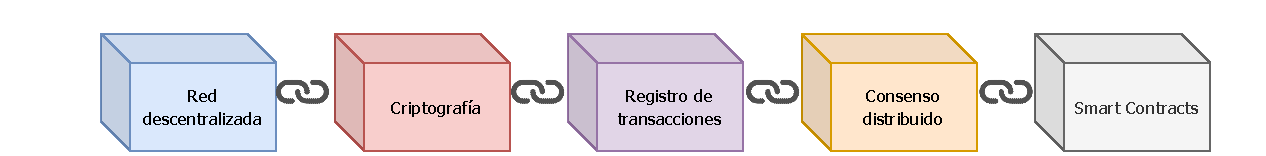
\includegraphics[width=\textwidth]{figuras/blockchain diagram.pdf}
    \caption{Diagrama indicando los 5 componentes de una \textit{blockchain}. Fuente: elaboración propia.}
    \label{fig:blockchaindiag}
\end{figure}

\section{La Estructura de Cadena}
Normalmente, salvo en casos poco populares, el registro de la \textit{blockchain} sigue una estructura de cadena~\cite{survey-blockchain}. Los datos están organizados en bloques de datos: $\{b_1, b_2, \dots\}$. Cuando se necesita almacenar nuevas transacciones, estas se colocan en un nuevo bloque que se añadirá después del último bloque ya existente de la cadena. Además de almacenar la información de la transacción, el estado de la \textit{blockchain} si procede, e información necesaria en una cabecera, el bloque tiene dos atributos fundamentales:
\begin{itemize}
    \item \textbf{ID del bloque}: este es el \textit{hash} del contenido del bloque usando una función de \textit{hash} criptográfica $H$. Esta función está predefinida y se conoce de manera pública.
    \item \textbf{El hash anterior}: es el ID del bloque anterior.
\end{itemize}

Notemos que el ID del bloque no tiene por qué ser necesariamente almacenado en el bloque ya que se puede calcular a partir del contenido del bloque.

El \textit{hash} anterior es una información crítica para mantener la integridad de la cadena. Si cualquier parte de cualquier bloque cambiase después de registrarse en la \textit{blockchain}, este cambio será detectado. Esto es porque para añadir un nuevo bloque a la \textit{blockchain} se debe de cumplir un proceso llamado validación del bloque~\cite{duc-2023}. Un nuevo bloque $b_{i+1}$ es válido si:
\begin{enumerate}
    \item El \textit{hash} anterior es consistente, esto es: $b_{i+1}^{prev} = H(b_i)$.
    \item Todas las transacciones de $b_{i+1}$ son válidas.
    \item El bloque $b_i$ es válido.
\end{enumerate}

La verificación en el paso 1 necesita calcular el \textit{hash} de $b_i$ y compararlo con $b_{i+1}^{prev}$. El paso 3 necesita ejecutar el mismo proceso de validación para verificar la validez del bloque $b_i$. Consecuentemente, para validar el bloque $b_{i+1}$, se necesita comprobar todos los \textit{hash} anteriores de todos los bloques $b_j$ con $j \le i+1$. Si un bloque anterior, digamos, $b_{j-1}$ ha sido modificado, entonces cuando calculemos su \textit{hash}, $H(b_{j-1})$, encontraremos que es distinto del valor $b_j^{prev}$ almacenado en el bloque $b_j$. Esto resulta en una infracción y como resultado el nuevo bloque $b_{i+1}$ se considerará inválido y no se añadirá a la \textit{blockchain}.

Una consecuencia de haber modificado el bloque $b_j$ es que la \textit{blockchain} no podrá crecer más. Uno podría pensar que en ese caso la \textit{blockchain} se vuelve inútil ya que detiene a toda la \textit{blockchain}. Esto sería cierto si la red \textit{blockchain} estuviese compuesta de un único ordenador. En la práctica, la red \textit{blockchain} está compuesta de varios ordenadores~\cite{duc-2023}, donde los datos de la \textit{blockchain} están duplicados en cada nodo. Para que un nodo se asegure de que su copia de la \textit{blockchain} es correcta, necesita comparar su copia con la de sus vecinos para escoger la \textit{blockchain} más larga como la correcta~\cite{bitcoin}. Antes de realizar esta comparación, el nodo necesita verificar la validez de la copia de cada vecino, lo que implica validar todos los bloques de la copia. Por lo tanto, si la copia de la \textit{blockchain} de algún nodo incluye alguna infracción, esta copia no será considerada válida. Por lo tanto, los nodos honestos de la red nunca usarán una copia errónea~\cite{bitcoin}.

\section{Cómo Conseguir un Consenso}

El consenso ya era un área de investigación en computación con 30 años de estudio antes de que la tecnología \textit{blockchain} se volviese popular. Comenzó en los años 70 con el proyecto de la NASA, ``\textit{Software Implemented Fault Tolerance} (SIFT)``~\cite{sift}, enfocado a construir un sistema de control de naves resistente. El reto consistía en replicar el sistema en múltiples máquinas de manera que el sistema se pudiese resistir fallos de múltiples de ellas. Más adelante este reto se formuló como el ahora conocido ``Problema de los Generales Bizantinos``~\cite{byzantine-general}. Este problema popularizó el término ``Fallo Bizantino (\textit{Byzantine Fault})`` para indicar una condición de un sistema distribuido donde algunos nodos no son confiables y pueden aparentar normales o maliciosos de manera arbitraria, pudiendo camuflarse entre ellos de manera que no haya información consistente para que los otros nodos declaren su mal funcionamiento.

Un sistema sistema \ac{BFT}~\cite{sift} debe de evitar el fallo completo y por tanto los nodos deben de acordar una estrategia común y seguir este consenso, sabiendo que algunos nodos pueden fallar o actuar de manera maliciosa. Para describir \ac{BFT} de manera formal, consideremos un sistema de difusión donde un nodo necesita difundir un mensaje (valor) a todos los demás nodos de manera par a par. Al principio, en nodo emisor recibe un valor de entrada $m$. El protocolo de difusión debe concluir con que cada nodo $i$ tenga un valor de salida $m_i$. El emisor y los receptores pueden ser honestos o deshonestos. Este protocolo logra \ac{BFT} si cumple dos requisitos:
\begin{itemize}
    \item \textbf{Consistencia}: todos los nodos honestos $i$ y $j$ deben de tener el mismo valor: $m_i=m_j$.
    \item \textbf{Validez}: si el emisor es honesto, todos los nodos honestos $i$ deben de tener el mismo valor: $m=m_i$.
\end{itemize}

Un sistema puede ser consistente pero no válido, cuando todos los nodos honestos tienen el mismo valor de salida pero no es el mismo que el del emisor. Un sistema puede ser válido pero no consistente, cuando el emisor no es honesto y transmite valores distintos a los nodos. Por tanto, ninguno de los requisitos es condición suficiente.

Una \textit{blockchain} es un sistema \ac{BFT}. Para solventar las inconsistencias debido al trabajo autónomo e independiente de los nodos, la solución estándar es que cada nodo esté de acuerdo en que la copia más larga de la \textit{blockchain}, es decir, la que tiene más bloques, es la versión globalmente correcta. Debido a que las copias más cortas que la correcta no se usan, los nodos quieren tener sus copias lo más actualizadas posibles ya que si no podrían malgastar esfuerzos en añadir bloques a la \textit{blockchain} equivocada. Como consecuencia, aunque a veces algunas transacciones sean registradas en distintas copias de la \textit{blockchain} en nodos distintos, varias transacciones pueden ser añadidos al último bloque de la \textit{blockchain} existente en distintos nodos, o aunque distintos nodos pueden tener copias distintas de la \textit{blockchain}, al final estos nodos tendrán la misma copia de la \textit{blockchain}.

Sin embargo esto es solo en teoría. Si un consenso ocurre demasiado tarde, las inconsistencias mencionadas previamente causarán que el sistema rinda de manera incorrecta. Por lo tanto, necesitamos minimizar la probabilidad de estas inconsistencias y minimizar el tiempo que se tarda en alcanzar el consenso de la \textit{blockchain}. Para esto, se han usado distintos mecanismos de consenso en \textit{blockchain}. Entre los más comunes están la \ac{PoW} o la \ac{PoS}.

\section{Algoritmos de Consenso}
Para hacer una comunicación confiable entre los nodos y mantener el estado correcto a través del sistema incluso en presencia de nodos maliciosos o incluso ante fallos de la red, se usan los conocidos algoritmos de consenso brevemente expuestos anteriormente. El algoritmo de consenso es el responsable para mantener copias consistentes del estado actual de la \textit{blockchain} en todos los nodos, validar nuevas transacciones y actualizar el estado actual mientras se alcanza un acuerdo entre los nodos. Nos centraremos en explicar los dos algoritmos de consenso más populares, \ac{PoW} y \ac{PoS}.
\subsection{Proof Of Work}
El algoritmo de \ac{PoW} normalmente necesita un nodo de prueba y otro de verificación. El nodo de prueba realiza una tarea computacionalmente intensiva para encontrar una solución a un problema de una cierta dificultad. El resultado entonces se presenta al verificador que consume significantemente menos recursos para verificar el resultado. La asimetría y la excesiva cantidad de recursos necesitados por el nodo de prueba sirve para lograr dos propósitos:
\begin{enumerate}
    \item Mitiga ataques sibilinos a nivel de consenso. Lanzar un ataque sibilino necesita a un adversario creando múltiples entidades maliciosas o a varias entidades coordinadas entre sí. Sin embargo, por diseño, la cantidad de recursos computacionales es importante para el algoritmo de \ac{PoW}, no la cantidad de nodos.
    \item La carga de trabajo en sí se convierte en un seguro contra ataques de bifurcación. La longitud de la cadena es prácticamente proporcional a la cantidad de recursos gastados minando bloques. Si el adversario quiere modificar una transacción del pasado, necesita primero tener más del 51\% de los recursos computacionales dentro de la red, bifurcar una nueva cadena a partir del bloque objetivo, y minar los bloques hasta que la nueva cadena se vuelva la más larga.
\end{enumerate}

Normalmente los algoritmos de \ac{PoW} emplean tareas que computacionales que hacen uso de la CPU o de la GPU. La red más famosa que usa este tipo de algoritmo es la de Bitcoin. El algoritmo necesita encontrar un número llamado \textit{nonce} tal que, cuando es \textit{hasheado} con los contenidos del bloque (usando SHA-256d, esto es, SHA-256 aplicado dos veces), el resultado sea un número menor que un valor de dificultad. Cuando un \textit{nonce} adecuado se encuentra y es aprobado por los verificadores, el nodo que lo ha encontrado obtiene una recompensa. El proceso de encontrar este número se llama minar, y a los nodos que lo buscan se llaman mineros.

\subsection{Proof Of Stake}
Para solventar las desventajas de algoritmos de \ac{PoW} tales como minado centralizado y consumo energético, los algoritmos de \ac{PoS} están ganando fuerza. Un algoritmo de \ac{PoS} intenta validar transacciones y logra consenso en la red sin el uso de tareas computacionalmente intensas. En lugar de ``trabajar``, un nodo verificador tiene que bloquear su ``participación``, que es una parte de su riqueza en la red.

En un algoritmo de \ac{PoS}, los propietarios de la participación bloquean su ``participación`` y se vuelven elegibles para participar en la validación de la transacción y en la creación de un nuevo bloque. Estos no minan nuevas monedas a diferencia de los algoritmos de \ac{PoW}. En su lugar, recolectan las tasas de transacción o intereses proporcionales a su participación como recompensa. Si el nodo se identifica como malicioso, su participación y recompensa pueden ser confiscadas, lo que sirve como un aliciente económico para evitar nodos maliciosos.

Las ventajas de un algoritmo de \ac{PoS} sobre uno de \ac{PoW} son las siguientes:
\begin{itemize}
    \item \textbf{Descentralización}: en los algoritmos de \ac{PoW} los mineros pueden tener un incremento exponencial en recursos computacionales cuando se invierte en equipamiento centrado en el minado. En una red de \ac{PoS}, la ganancia es directamente proporcional a la cantidad de participación que el nodo decide invertir.
    \item \textbf{Eficiencia energética}: los algoritmos de \ac{PoW} consumen mucha energía. En el caso de Bitcoin, sus mineros consumen más energía que países como Portugal, Singapur o la República Checa. Los algoritmos de \ac{PoS} no necesitan que los nodos resuelvan tareas computacionalmente intensas cuando se crean nuevos bloques. Por lo tanto pueden ser altamente eficientes a nivel energético.
\end{itemize}

\part{Propuesta: Krum Federated Chain}\label{sec:kfc}


 \chapter{blockchain aplicado a Federated Learning}\label{sec:blockfed}
Debido a las propiedades de la tecnología \textit{blockchain} han sido múltiples los trabajos para combinar \ac{FL} y esta tecnología~\cite{zhu-2023-blockfed} con el fin de resolver problemas causados mayormente por la centralización en \ac{FL}. La combinación de \textit{blockchain} y \ac{FL} es ampliamente usada  en múltiples campos~\cite{kim-2020-blockfl, weng-2021-deepchain} y ha mostrado un gran éxito que ha llevado a muchas propuestas. Aún así, como veremos, es un campo todavía muy reciente y por tanto sin ningún estándar establecido al que ceñirnos.

\section{Blockchain como solución a problemas del federated learning}

Una de las principales aplicaciones de la tecnología \textit{blockchain} en \ac{FL} es la propuesta de soluciones a algunos problemas derivados del aprendizaje distribuido en \ac{FL}. A continuación exponemos algunos de estos problemas vigentes en esquemas federados, muchos de ellos causados por la centralización de los esquemas clásicos de \ac{FL} y ofrecemos una breve vista sobre como el uso de tecnología \textit{blockchain} nos puede ayudar a solventar estos problemas o, al menos, mejorar las soluciones actuales.

\subsection{Falta de incentivos}
Cuando un cliente participa en una tarea de \ac{FL}, consume una cantidad de recursos, incluyendo computación, ancho de banda de la red y batería. Además son varios los riesgos de seguridad que suele llevar el esquema federado como hemos visto en secciones anteriores. Esto hace que en algunos casos los clientes no quieran formar parte de la tarea de \ac{FL} a no ser que obtengan un beneficio. 

Aunque los mecanismos de incentivo son un campo de investigación activo en \ac{FL}~\cite{wang-2018, xu-2015}, la mayoría de soluciones propuestas necesitan una entidad central en la que se pueda confiar para observar el comportamiento de los clientes y dar sus recompensas. Este problema proviene de la centralización del esquema de \ac{FL} y por tanto es un buen candidato a ser resuelto mediante el uso de \textit{blockchain}. El problema se puede resolver haciendo uso de los mecanismos de recompensa económicos que integran múltiples redes \textit{blockchain}. Por ejemplo, \citet{zhao-2021} propuso un sistema de reputación basado en \textit{blockchain} para \ac{FL} para dispositivos \ac{IoT} con el fin de entrenar modelos en los datos de los clientes.

\subsection{Heterogeneidad estadística}

La heterogeneidad estadística se refiere a las distintas distribuciones de datos de los clientes. Esto aumenta de manera drástica la complejidad del modelado del problema, análisis teórico y evaluación empírica de las soluciones. Por una parte, es difícil modelar los datos heterogéneos cuando se entrenan modelos federados en conjuntos no idénticamente distribuidos en los clientes. Por otro lado, no es fácil analizar la convergencia en procesos de entrenamiento en los que los datos son heterogéneos. En \textit{blockchain} se ha trabajado en algoritmos de optimización distribuidos logrando resolver las limitaciones de las soluciones existentes. Por ejemplo, el algoritmo de promedio con pesos según las distancias basado en \textit{blockchain} propuesto por~\citet{zhang-2021} ha demostrado tener una buena precisión a la hora de tratar el problema de heterogeneidad de datos en \ac{FL}. Además, se pueden desplegar redes \textit{blockchain}.

\subsection{Heterogeneidad de sistemas}
La heterogeneidad de sistemas se refiere a las diferencias sustanciales en capacidad de computación, ancho de banda de red, batería, capacidad de almacenamiento, etc., de los dispositivos en la red de \ac{FL}. Además, las restricciones del tamaño de la red de cada dispositivo o a nivel de sistema normalmente solo soportan un pequeño porcentaje de estos estando activos inmediatamente. Por lo tanto, una arquitectura de \ac{FL} debe de tolerar \textit{hardware} heterogéneo y ser lo suficientemente robusta como para descartar dispositivos en la red de comunicación. El uso de tecnología \textit{blockchain} también puede ayudar a abordar este problema. Un ejemplo es la propuesta de~\citet{zhang-2021} de un sistema de \ac{FL} basado en \textit{blockchain} para la detección de errores en dispositivos industriales \ac{IoT}, el cual puede lograr la integridad verificable de los datos de los clientes.

\subsection{Seguridad del modelo}
Como se mostró en la Sección~\ref{sec:ataquesfl} un esquema de \ac{FL} no es totalmente seguro y pueden participar clientes maliciosos con el fin de destruir los modelos finales. Además los modelos pueden ser filtrados por servidores no fiables llevando así también a problemas de privacidad. Las soluciones actuales no pueden eliminar la posibilidad de que un servidor central robe datos o modifique el modelo para dañarlo~\cite{zhu-2023-blockfed}. Los esquemas basados en \textit{blockchain} no requieren de un servidor central para la agregación del modelo lo que reduce riesgos en el sistema distribuido. Además, la verificación de identidad, trazabilidad, durabilidad, anonimidad y alta escabilidad de esta tecnología también permite garantizar la seguridad del modelo.

\subsection{Privacidad de los datos}
Aunque en \ac{FL} se compartan modelos y no datos, la comunicación de las actualizaciones del modelo entre clientes y servidor permite la extracción de información sensible a terceros o al servidor central. Además, algunos clientes maliciosos también pueden inferir información a partir de parámetros compartidos. Algunos métodos actuales pasan por el uso de \ac{DP} o métodos de  cifrado como vimos en la Sección~\ref{sec:fldp}, aunque tienen el problema de perjudicar el rendimiento del modelo. En métodos de \textit{blockchain} se ha propuesto con éxito~\cite{mcmahan-2018} la incorporación de \ac{DP} local a nivel de cliente. También la seguridad criptográfica de la \textit{blockchain} permite el cifrado del modelo global en la red dejando solo a los clientes con la clave para descifrar este, evitando así ataques externos.


\subsection{Coste de las comunicaciones}
Dado que el cómputo de entrenamiento está repartido entre dispositivos conectados a través de internet, las comunicaciones son un cuello de botella en una red federada. Una red federada puede contener gran cantidad de dispositivos diferentes, como millones de teléfonos móviles. Debido a los recursos limitados, como el bando de ancha de la red, energía o potencia, la comunicación en la red puede ser incluso más lenta que el cómputo local. Por lo tanto, es necesario desarrollar un método de comunicación eficaz. Se ha probado que usando un mecanismo de consenso adecuado y ajustando los parámetros básicos de la \textit{blockchain} se puede solventar este problema. Por ejemplo, en el trabajo propuesto por~\citet{kim-2020-blockfl} el sistema optimiza la latencia de fin a fin del modelo ajustando la tasa de generación de bloques de la red. Además, también propusieron un método para calcular la latencia mediante el ajuste de la dificultad en \ac{PoW}. \citet{majeed-2019} han empleado una \textit{blockchain} con permisos mejorando la eficiencia de transmisión significantemente.

\section{Mecanismos de consenso en blockchain aplicado a Federado}

Los mecanismos de consenso son un elemento clave de la arquitectura de la \textit{blockchain}. Aunque \ac{PoW} es todavía el principal método usado en este campo y el más estudiado en la literatura, tanto a nivel teórico como de propuestas de arquitecturas, no se considera práctico desplegar \ac{PoW} directamente en un sistema de \ac{FL} por motivos de eficiencia. Por lo tanto, esto ha llevado al diseño de varios métodos de consenso. Algunas propuestas usan \ac{PoS} como mecanismo de consenso~\cite{awan-2019, preuveneers-2018} debido a su bajo consumo energético aunque requieren el uso de algún mecanismo de incentivo económico, por lo que su uso es restringido. Una de las propuestas más interesantes es \ac{PoFL}~\cite{qu-2021-pofl}. 

El mecanismo de consenso \ac{PoFL}~\cite{qu-2021-pofl} fue desarrollado como solución eficiente a nivel energético para la integración de la tecnología blockchain con \ac{FL}. Inspirado por el concepto de los mecanismos de consenso \textit{Proof-of-Useful Work}~\cite{sabry-2023-pouw}, \ac{PoFL} mantiene la idea fundamental de \ac{PoW}: hacer que los participantes resuelvan problemas computacionalmente intensivos para lograr un consenso. Sin embargo, a diferencia de \ac{PoW}, que utiliza la potencia computacional para tareas sin ningún valor inherente (por ejemplo, encontrar un \textit{nonce} en la red de Bitcoin~\cite{duc-2023}), \ac{PoFL} decide usar estos recursos para entrenar un modelo federado.

\subsection{El mecanismo de consenso PoFL}
Es importante saber que \ac{PoFL} hace uso una arquitectura de \textit{pooled-mining}. En esta estructura, los participantes de la red son divididos entre diferentes \textit{pools}, cada una supervisada por un minero asignado. Estas \textit{pools} operan de manera independiente, entrenando sus respectivos modelos federados sin ninguna comunicación entre \textit{pools}. La \textit{pool} que entrene el modelo con mayor precisión en un conjunto de datos de prueba previamente determinado será considerada la ganadora en la ronda de consenso. Como consecuencia, el modelo ganador se integra en la blockchain y es retransmitido a través de toda la red a los clientes. El proceso dentro de cada \textit{pool} se ilustra en la figura \ref{fig:pooledmining}:
\begin{enumerate}
	\item El minero difunde el modelo inicial a los clientes.
	\item Los clientes entrenan su copia local del modelo usando sus datos privados. Este paso incluye el calcular las actualizaciones locales basadas en la diferencia entre el modelo recibido y el modelo entrenado.
	\item Los clientes mandan las actualizaciones locales al minero. El minero agrega estas actualizaciones para crear un nuevo modelo mejorado. El minero evalúa el rendimiento del modelo agregado contra una meta de rendimiento previamente establecida. Si se alcanza esta meta, se llega a consenso en esa ronda.
	\item Después de llegar al consenso, el minero añade el modelo mejorado a la blockchain y lo retransmite a todos los mineros, y por tanto a todos los clientes participando. Si no se llega a consenso (no se consigue la meta), el proceso se reinicia desde el paso 2, con los clientes entrenando hasta que se alcance la meta deseada.
\end{enumerate}

\begin{figure}[ht]
	\centering
	\usetikzlibrary{positioning}
\usetikzlibrary{calc}
\usetikzlibrary{babel}
\definecolor{pastelred}{HTML}{D37676}
\begin{tikzpicture}[
scale=2,
clientnode/.style={rectangle, draw=black!100, text width=1.5cm,
align=center, anchor=center, fill=blue!30},
textnode/.style={}
]

%Nodes
\node[clientnode] (miner) {Minero};
\node[textnode] (dots) [below=2cm of miner] {\large ...};
\node[clientnode] (client1) [left=of dots] {Cliente};
\node[clientnode] (client2) [right=of dots] {Cliente};
\node[textnode] (label1) [below=0.05cm of client1] {\textsuperscript{(2) Entrenamiento Local}};
\node[textnode] (label2) [left=0.05cm of client2] {};

%Coordinates
\coordinate (miner1) at ($ (miner.south) - (0.2,0) $);
\coordinate (miner2) at ($ (miner.south) - (0.05,0) $);
\coordinate (miner3) at ($ (miner.south) + (0.05,0) $);
\coordinate (miner4) at ($ (miner.south) + (0.2,0) $);
\coordinate (client11) at ( $ (client1.north) - (0.1, 0) $ );
\coordinate (client12) at ( $ (client1.north) + (0.1, 0) $ );
\coordinate (client21) at ( $ (client2.north) - (0.1, 0) $ );
\coordinate (client22) at ( $ (client2.north) + (0.1, 0) $ );

%Lines
\draw[thick, ->] (miner1) -- (client11) node[midway, above left] {};
\draw[thick, ->] (miner4) -- (client22) node[midway, above right] {};
\draw[thick, ->] (client12) -- (miner2) node[midway, below right] {};
\draw[thick, ->] (client21) -- (miner3) node[midway, below left] {};

\draw[dashed, ->] (miner.west) .. controls +(left:1.2cm) .. (client1.west) node[midway, above left] {\textsuperscript{(4) Modelo Mejorado}};
\draw[dashed, ->] (miner.east) .. controls +(right:1.2cm) .. (client2.east) node[midway, above right] {};


\node[textnode, above=1cm of client11] {\textsuperscript{(1) Modelo Inicial}};
\node[textnode, above right=0.4cm and 3.7cm of client12] {\textsuperscript{(3) Actualizaciones del Modelo}};
    
\end{tikzpicture}
	\caption{Diagrama mostrando como funciona el procedimiento de \textit{pooled-mining}. Fuente: Elaboración propia.}
	\label{fig:pooledmining}
\end{figure}

Formalmente, podemos modelar una red de blockchain usando \ac{PoFL} como un conjunto de \textit{pools} $\{P_1, P_2, \ldots, P_n\}$, donde cada \textit{pool} $P_i$ contiene un minero $m_i$ y un conjunto de clientes $\{C_1^i, \ldots, C_{j_i}^i\}$. En cada ronda de aprendizaje $t$, cada \textit{pool} $P_i$ computa un modelo federado denotado por $L_i^t$ mediante un proceso de entrenamiento federado coordinado por e minero $m_i$. Entonces, cada minero $m_i$ calcula la precisión de su modelo $L_i^t$ en un conjunto de datos determinado $\mathcal{D}$, que denotaremos por $accuracy(L_i^t, \mathcal{D})$. El minero $m_i*$ ganará el consenso si
\begin{equation}
	accuracy(L_i^t, \mathcal{D}) \le accuracy(L_{i*}^t, \mathcal{D}) \quad \forall i \in \{ 1, \ldots, n\}.
\end{equation}

Después de llegar a consenso, el modelo $L_{i*}^t$ es difundido a todos los mineros $m_j$ con $j \ne i*$ los cuales comprobarán que la precisión calculada es correcta. Después de una verificación correcta, el minero $m_{i*}$ creará un nuevo bloque $b_t$ en que se establecerá $G^{t+1}=L_{i*}^t$ y la añadirá a la blockchain. Finalmente, todos los mineros descargarán la nueva versión de la blockchain y difundirán el nuevo modelo global $G^{t+1}$ a todos sus clientes, asegurándose así que todos los clientes tienen acceso al último modelo.


Aunque son varios los mecanismos propuestos la mayoría de estudios no están dedicados a escenarios de \ac{FL} por lo que su implementación puede no ser idónea para nuestro caso. Actualmente existe una alta demanda para desarrollar mecanismos de consenso eficientes a nivel energético para la redes \textit{blockchain} en \ac{FL}.

\section{Arquitecturas en blockchain aplicado a FL}

Debido a la amplia cantidad de arquitecturas propuestas, no han sido pocos los trabajos que han intentado categorizarlas. Una de las categorizaciones más interesantes es la de~\citet{zhu-2023-blockfed} que propone categorizar las arquitecturas según el conjunto de mineros y clientes de la red en tres tipos: desacoplado, acoplado y superpuesto. En lo que sigue $M$ hará referencia al conjunto de los mineros de la red y $C$ al conjunto de los clientes de la red.

\subsection{Modelo Desacoplado}
Se dice que nuestra red sigue un modelo desacoplado cuando dado un nodo, este solo trabaja en un esquema federado o en \textit{blockchain}, pero nunca en ambos. Formalmente se puede expresar como $C \cap M = \emptyset$. De este modo, los los clientes únicamente se encargarán de entrenar los modelos locales y de mandar las actualizaciones a los mineros. Estos últimos serán los encargados agregar los modelos, ejecutar el mecanismo de consenso, validar transacciones y escribir en la \textit{blockchain}. 

Este modelo tiene múltiples ventajas como la facilidad a la hora de su implementación o bajos requisitos energéticos para muchos nodos dado que no tienen que ejecutar el mecanismo de consenso todos. Sin embargo sí implica un mayor coste en comunicaciones, dificultad a la hora de implementar mecanismos de incentivo o seleccionar clientes adecuados.
\begin{figure}[h]
	\centering
	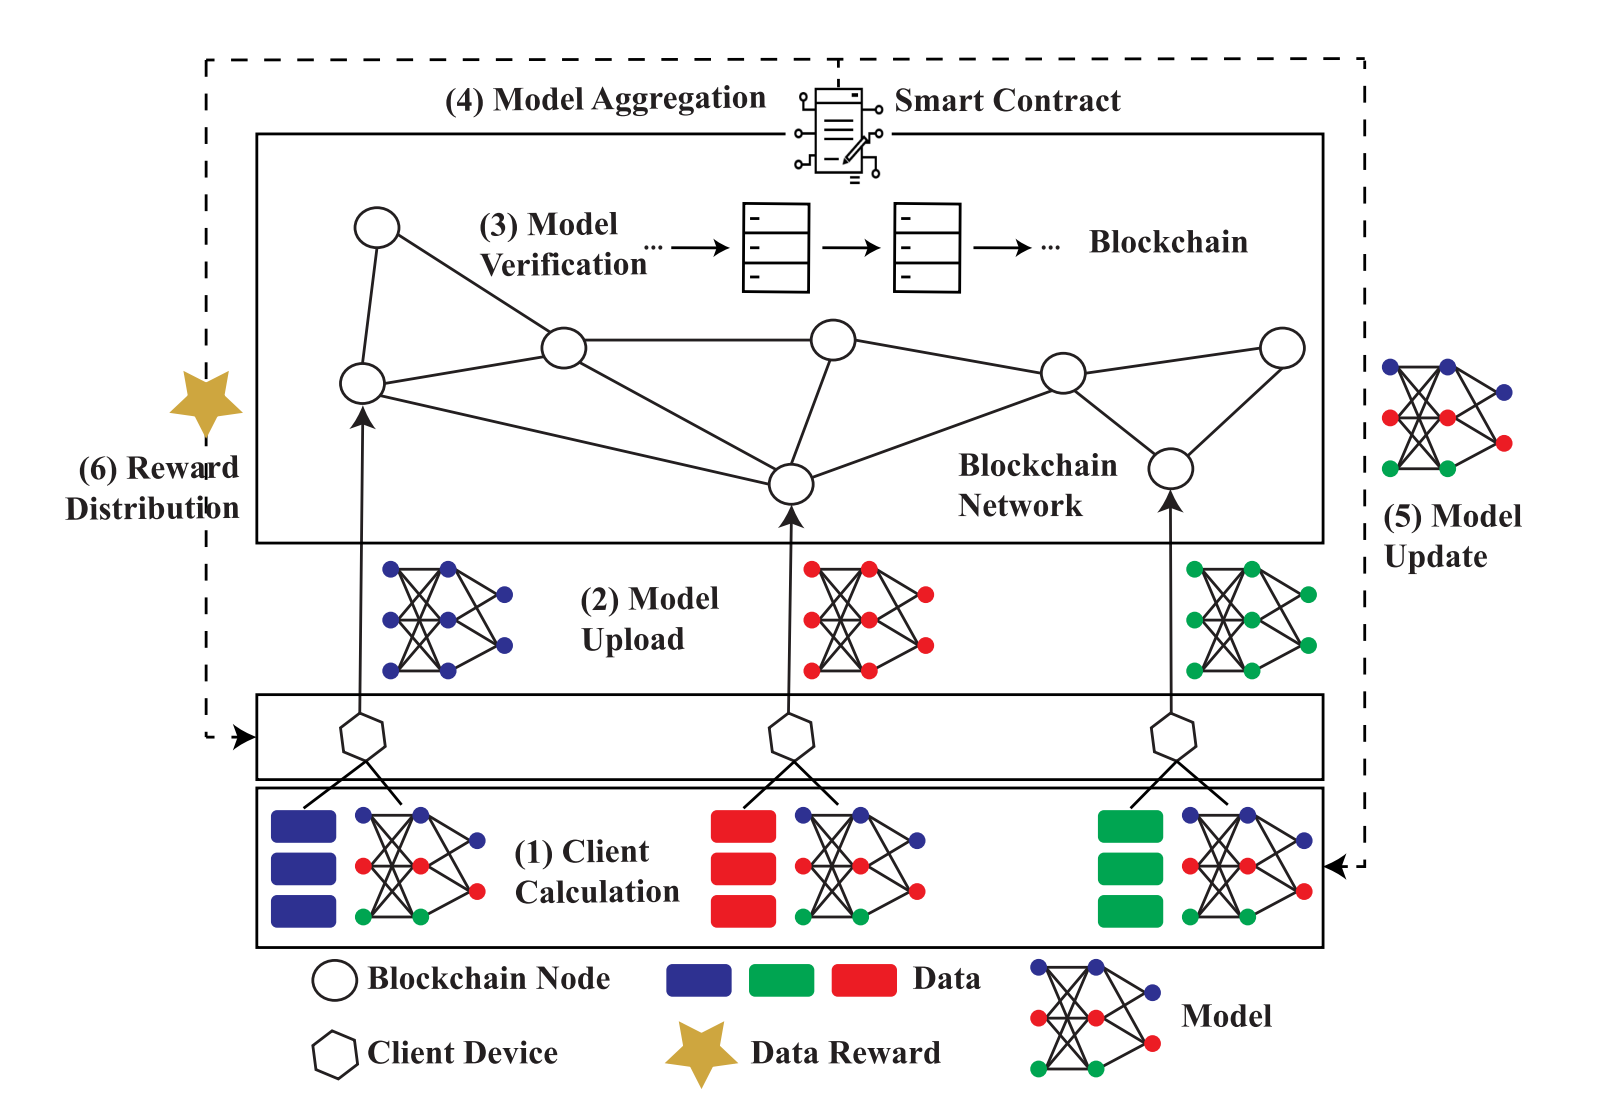
\includegraphics[width=0.8\textwidth]{figuras/decoupled.png}
	\caption{Esquema de una arquitectura según el modelo desacoplado. Fuente: \cite{zhu-2023-blockfed}.}
	\label{fig:decoupled}
\end{figure}

\subsection{Modelo Acoplado}
En el modelo acoplado, todos los nodos son responsables de participar en el esquema de \ac{FL} y de \textit{blockchain}. Formalmente se puede expresar como $C=M$. En este modelo, los nodos se pueden llamar nodos compuestos y realizan tanto el entrenamiento local como la agregación, generación de transacciones y verificación, sumando a esto la generación de bloques y su validación. 

Esto lleva a que los nodos tengan pocos costes de comunicaciones debido a la topología de la red. Además debido a la integración total de la \textit{blockchain} y el esquema federado, el modelo acoplado es también simple de configurar y de diseñar. Sin embargo, cada nodo realiza tareas intensivas a la hora de entrenar el modelo y de ejecutar el mecanismo de consenso. Otro problema es que cada nodo en el esquema tiene más responsabilidades que en otros esquemas, creando así más preocupaciones a nivel de privacidad de datos o seguridad del modelo.
\begin{figure}[h]
	\centering
	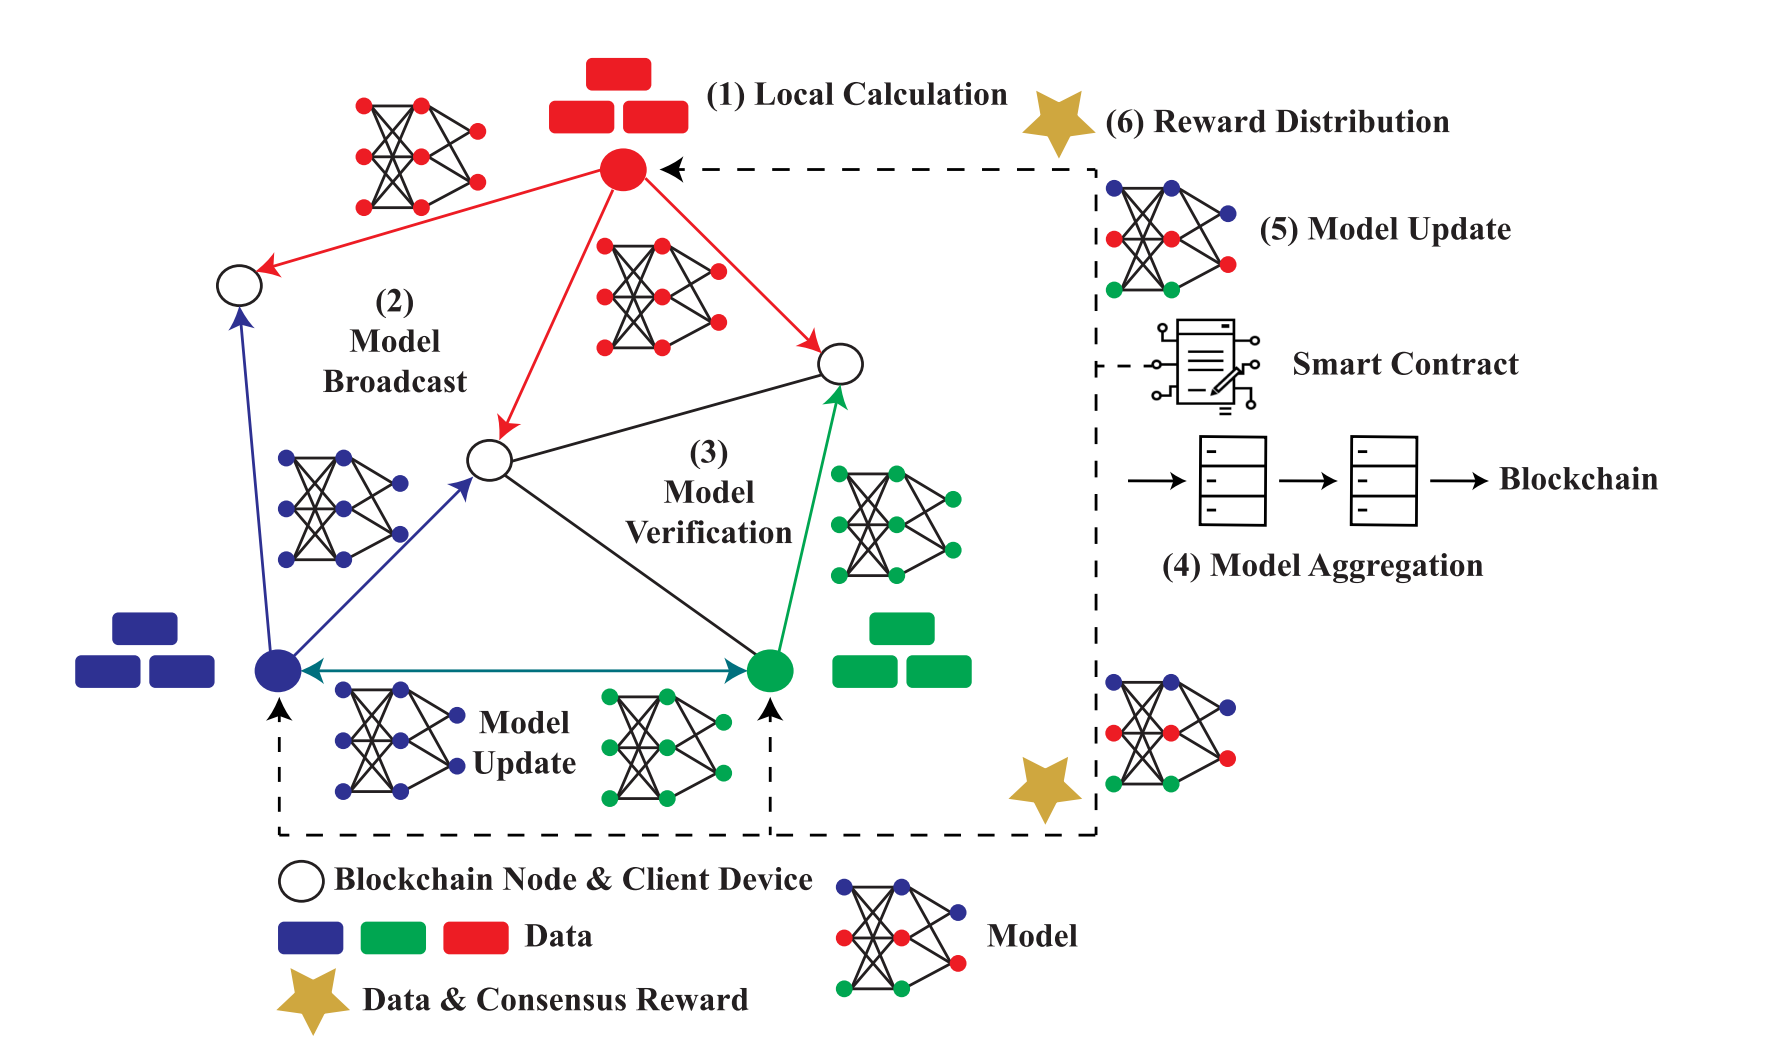
\includegraphics[width=0.8\textwidth]{figuras/coupled.png}
	\caption{Esquema de una arquitectura según el modelo acoplado. Fuente: \cite{zhu-2023-blockfed}.}
	\label{fig:coupled}
\end{figure}

\subsection{Modelo superpuesto}
En el modelo superpuesto encontramos tres tipos de nodos: nodos de \textit{blockchain}, nodos de \ac{FL} y nodos compuestos. Formalmente lo podemos expresar como $M \cap C \ne \emptyset, M\ne C$. Pese a las distintas funciones, un nodo puede cambiar su tipo a lo largo del tiempo. El modelo superpuesto equilibra el modelo acoplado y desacoplado y toma la ventajas de ambos. Sin embargo esto se ve reflejado en complejidad a la hora de configurar la red. 

La asignación de las funciones de los nodos se puede optimizar basado en los recursos disponibles, nivel de seguridad, etc. Sin embargo, a parte de las desventajas ya mencionadas, el modelo superpuesto tiene complicaciones a la hora de diseñar mecanismos de consenso e incentivo. Esto se debe a la dificultad intrínseca de la red.
\begin{figure}[h]
	\centering
	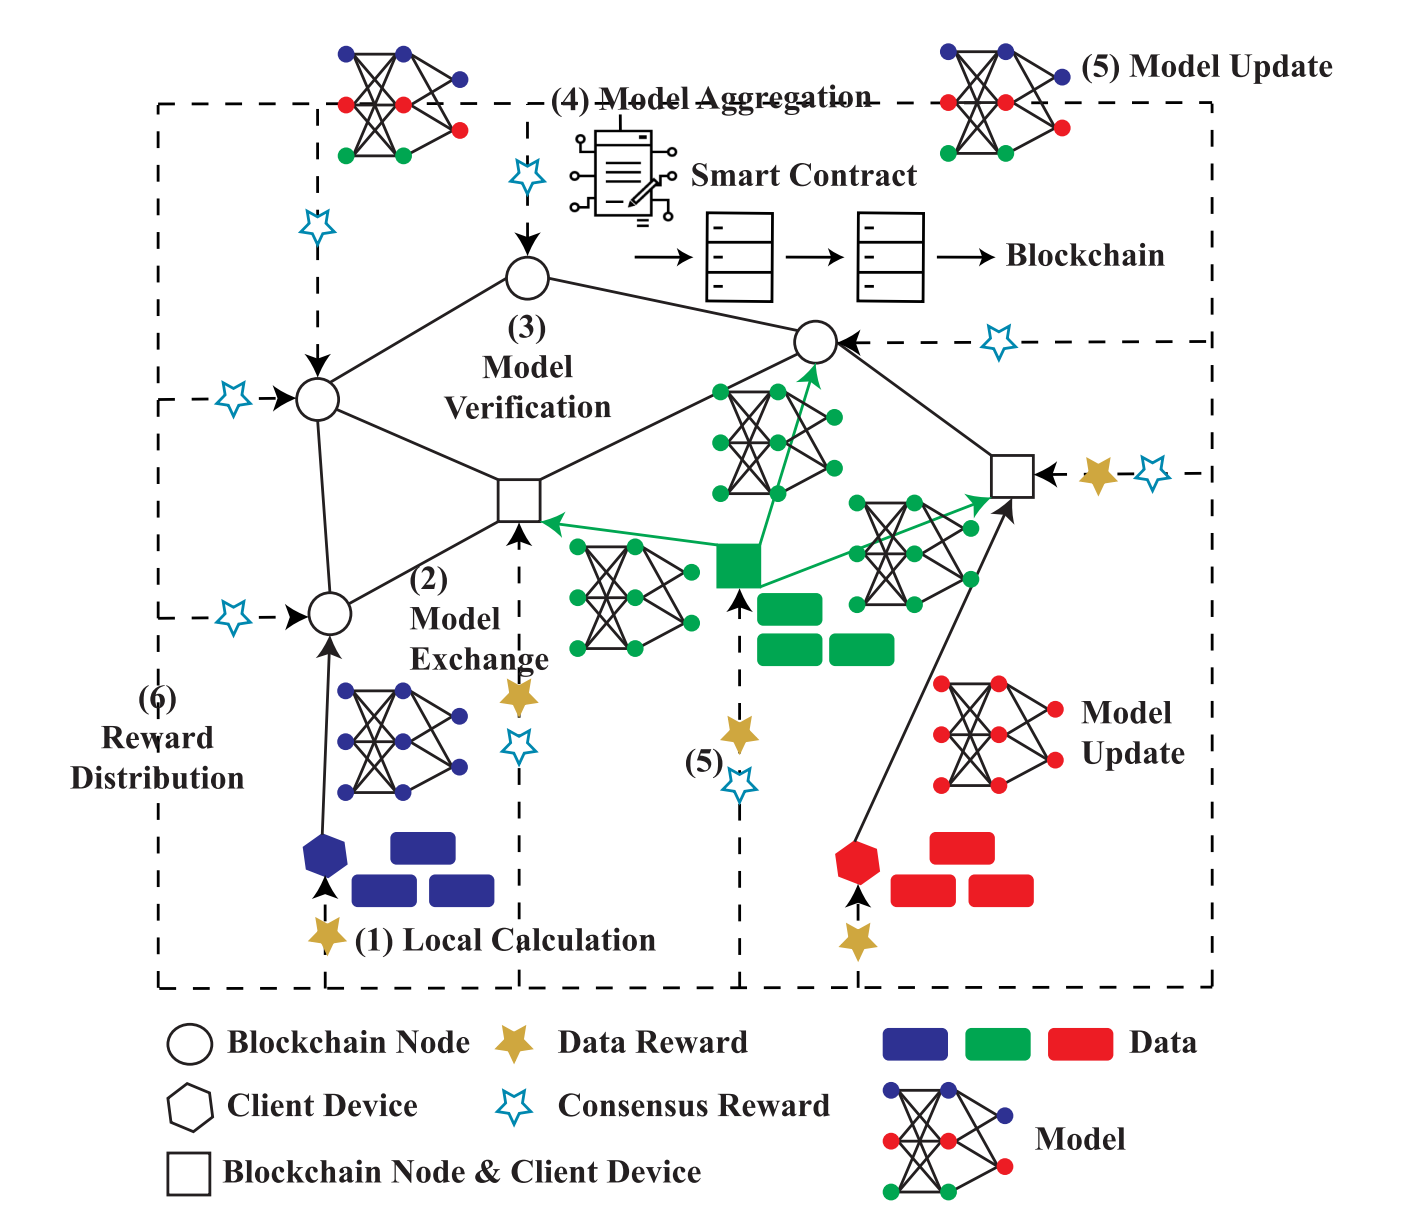
\includegraphics[width=0.8\textwidth]{figuras/overlapped.png}
	\caption{Esquema de una arquitectura según el modelo superpuesto. Fuente: \cite{zhu-2023-blockfed}.}
	\label{fig:overlapped}
\end{figure}

Como veremos más adelante, la mayoría de propuestas para combinar \ac{FL} y \textit{blockchain} consistirán en modelos acoplados o desacoplados que seguirán un estilo similar al de una red como \textit{Bitcoin}. Estas redes cuentan con lo que se conoce como mecanismo de \textit{Gossip}. Este mecanismo es un protocolo que permite a los mineros intercambiar información con el fin de que un minero $m_i$ pueda publicar en un bloque las transacciones recibidas o generadas por el minero $m_j$. Es por ello que la mayoría de arquitecturas se pueden ver como un esquema federado centralizado en el que en cada ronda $t$ el agregador central es un minero $m_{i_t}$. Este acercamiento nos permite beneficiarnos de todas las ventajas expuestas al principio del capítulo y con un diseño sencillo a nivel de red.
 \chapter{Propuesta: Krum Federated 
Chain (KFC)}\label{sec:propuesta}

Una vez introducidos todos los conceptos necesarios, en esta sección exponemos nuestra propuesta de mecanismo de defensa frente a ataques adversarios en \ac{FL} llamada \ac{KFC}. La propuesta parte de la hipótesis de que el mecanismo de consenso \ac{PoFL} puede ser una defensa contra ataques adversarios en \ac{FL}. Además, de las vulnerabilidades identificadas respecto a la configuración de los ataques, proponemos \ac{KFC}, una defensa basada en la combinación de Krum y blockchain con el mecanismo de consenso \ac{PoFL} para defender esquemas de \ac{FL} contra cualquier configuración de ataques adversarios.

\section{Hipótesis: PoFL como mecanismo de defensa}
Se puede apreciar que el mecanismo de consenso \ac{PoFL} exhibe una potencial defensa contra ataques adversarios. Los ataques bizantinos consisten en perjudicar el rendimiento del modelo federado y los ataques de \textit{backdoor} involucran a un adversario dentro de una \textit{pool} intentando manipular el proceso de entrenamiento del modelo para introducir una tarea secundaria. En el segundo caso, el hecho de estar optimizando varios objetivos pueden llevar a una ligera degradación en el rendimiento del modelo en la tarea original. 

Mediante el uso de un mecanismo de consenso basado en el rendimiento del modelo y \textit{pooled-mining}, \ac{PoFL} desalienta estos tipos de ataques. Las \textit{pools} que contengan a clientes adversarios son probables de producir modelos con una precisión inferior en el conjunto de datos preestablecido en comparación con las \textit{pools} sin clientes maliciosos. Como consecuencia, el mecanismo de consenso \ac{PoFL} favorecería a las \textit{pools} con el modelo con mejor rendimiento, filtrando de manera eficaz al modelo con la tarea inyectada y por tanto mitigando el ataque.

\section{Krum Federated Chain}

Es importante saber que la potencial resistencia de \ac{PoFL} contra ataques adversarios depende de la condición de que siempre exista una \textit{pool} sin ningún cliente malicioso en ella. Esta condición puede ser considerada demasiado optimista y exigente para el mundo real. Por lo tanto, proponemos la arquitectura \ac{KFC} como una alternativa a \ac{PoFL} con una seguridad más robusta. Aunque \ac{KFC} mantiene la misma arquitectura fundamental y principios de eficiencia energética que \ac{PoFL}, incorpora mecanismos de seguridad adicionales para mitigar ataques adversarios incluso en la presencia de actores maliciosos en todas las \textit{pools} de la red.

\ac{KFC} hace uso del operador de agregación Krum~\cite{krum-2017}, expuesto previamente en la sección \ref{sec:krum}, para mejorar su resistencia contra ataques al modelo federado. Recordamos que este operador funciona ordenando actualizaciones de clientes según la distancia geométrica entre las distribuciones de actualizaciones de modelo respectivas. Para ello y recuperando la notación de la Sección~\ref{sec:krum}, a cada cliente $i$ se le asigna la puntación

\begin{equation}
    s(i) = \sum_{i\to j} || V_i - V_j ||^2
\end{equation}

donde $i \to j$ denotaba el hecho de que el vector $V_j$ pertenecía al conjunto de los $n-f-2$ vectores más cercanos al vector $V_i$, con $i \ne j$. A continuación, selecciona la actualización más cercana a la mayoría, lo que efectivamente filtra a los outliers. Esto es, el vector $V$ resultado de la regla de agregación $KR(V_1, \ldots, V_n)$ se define como aquel vector $V_{i_*}$ tal que
\begin{equation}
    s(i_*) \le s(i) \quad \forall i \in \{ 1, \ldots, n\}.
\end{equation}


Los clientes adversarios que intentan manipular el modelo tienen más probabilidades de generar actualizaciones que se desvían significativamente de la norma, lo que los hace más propensos a ser identificados y excluidos por el operador Krum. 

Así, \ac{KFC} consiste en la combinación de la arquitectura base de \ac{PoFL} con la regla de agregación Krum para reforzar la seguridad a nivel de \textit{pool}. Esta decisión de diseño permite a \ac{KFC} verse beneficiado por la resistencia a ataques adversarios innata de \ac{PoFL} debido al uso de \textit{pooled-mining} y su mecanismo de consenso. Además, Krum refuerza esta resistencia mediante el filtrado de \textit{outliers} dentro de las distribuciones de las actualizaciones dentro de cada \textit{pool}. Por lo tanto, no hace falta mantener la hipótesis de la existencia de una \textit{pool} sin ningún tipo de actor malicioso. Este acercamiento combinado hace uso de distintos tipos de mecanismos de defensa en distintas partes del esquema federado, llegando así a una solución más robusta para \ac{FL} bajo condiciones adversarias.

\chapter{Entorno experimental}\label{sec:experimentos}

Con el fin de evaluar y medir el rendimiento de \ac{KFC} y \ac{PoFL}, hemos calculado la precisión o \textit{accuracy} del modelo federado resultante en múltiples conjuntos de datos expuestos en la Sección \ref{sec:evaldatasets} donde el objetivo era resolver un problema de clasificación de imágenes. Para esto hemos desplegado modelos basados en \ac{CNN} en un entorno de \ac{FL} explicados en la Sección \ref{sec:modelos}. Finalmente, explicamos los ataques cubiertos en la Sección \ref{sec:ataques}, los escenarios en los que se realizan en la Sección \ref{sec:escenarios} y las métricas usadas para la evaluación en la Sección \ref{sec:metricas}.

\section{Conjuntos de datos para la evaluación}\label{sec:evaldatasets}
Dado que \ac{PoFL}, y por tanto \ac{KFC}, necesitan un conjunto de validación con el fin de medir la precisión de cada modelo de la red, usamos el 20\% del conjunto de test de cada conjunto de datos con este fin dejando el 80\% restante como conjunto de test. Hemos usado tres conjuntos de datos en la evaluación, los cuales describimos a continuación:

\begin{enumerate}
    \item El conjunto de datos EMNIST (\textit{Extended Modified NIST}), presentado en 2017 en \cite{emnist}, es una extensión del famoso conjunto de datos MNIST~\cite{lecun-1998}. La clase \textit{EMNIST Digits} contiene un subconjunto balanceado del conjunto de dígitos. Esta contiene 28,000 muestras de cada dígito. Por lo tanto, el conjunto total consiste en 280,000 muestras, de las cuales 240,000 son usadas para el entrenamiento del modelo y 40,000 como muestras de test (usamos 8,000 como muestras de validación y las 32,000 restantes para test). Para los experimentos hemos decidido establecer el número de clientes en 200 y el de mineros en 3.
    
    \item El conjunto de datos Fashion MNIST \cite{fashionmnist-2017} fue diseñado para ser un reemplazo más exigente del conjunto original MNIST. Contiene un conjunto de 10 clases distintas extraídas del conjunto de imágenes de Zalando con 7,000 muestras de cada clase. Así, el conjunto de datos consiste de 70,000 muestras, de las cuales 60,000 son usadas para entrenamiento y 10,000 para test (usamos 2,000 para validación y las 8,000 restantes para test). Hemos establecido el número de clientes a 200 y el número de mineros a 3.

    \item El conjunto de datos CIFAR-10 es un subconjunto etiquetado del conjunto \textit{80 million tiny images}~\cite{torralba-2008}. Consta de 60,000 imágenes a color de resolución 32x32 de 10 clases, es decir, con 6,000 imágenes por clase. 50,000 imágenes son usadas para entrenamiento y 10,000 como validación, lo que corresponde a 1,000 muestras por clase (usamos 2,000 para validación y las 8,000 restantes para test). Establecemos el número de clientes a 100 (con el fin de tener más datos por cliente pues el modelo a entrenar es mucho más complejo) y el de mineros a 2.
\end{enumerate}


\begin{table}
    \centering
    \begin{tabular}{lrrr}
    \toprule
         &  \textbf{EMNIST}&  \textbf{Fashion MNIST}& \textbf{CIFAR-10}\\
         \toprule
         \textbf{Train}&  240,000&  60,000& 50,000\\
         \midrule
         \textbf{Test}&  32,000&  8,000& 8,000\\
         \midrule
         \textbf{Validation}&  8,000&  2,000& 2,000\\
         \bottomrule
    \end{tabular}
    \caption{Cantidad de muestras en cada conjunto distribuidas según su uso.}
    \label{tab:trainvaltest}
\end{table}

\section{Modelos de clasificación de imágenes}\label{sec:modelos}

Dado que todos los problemas que abordamos son problemas de clasificación, y que el objetivo principal de la propuesta no es maximizar el rendimiento si no probar mecanismos de defensa, usamos modelos de clasificación que obtengan buen rendimiento en estos problemas sin ataques. Para ello hemos considerado dos modelos:

\begin{itemize}
    \item En los conjuntos EMNIST y Fashion MNIST hemos usado una red \ac{CNN} estándar compuesta de dos capas convolucionales seguida cada una por una capas de \textit{max-pooling}, y un clasificador compuesto de dos capas densas con funciones de activación ReLU.
    \item En el conjunto más exigente CIFAR-10, hemos decidido usar una red de la familia ya expuesta previamente EfficientNet, concretamente una \texttt{EfficientNet-B0}. Hemos realizado un \textit{fine-tuning} usando unos pesos preentrenados de la red en el conjunto \textit{ImageNet}.
\end{itemize}

\section{Ataques adversarios}\label{sec:ataques}

A continuación se detallan los ataques implementados, basados en los ya introducidos en la Sección \ref{sec:adversarialattacks}. Con el fin de que las actualizaciones de los clientes adversarios no sean mitigadas al ser agregadas debido a la cantidad de clientes benignos, usamos técnicas de \textit{model replacement} para aumentar la eficacia del ataque.

\subsection{Ataques bizantinos}
Implementamos un ataque bizantino basado en \textit{random label flipping}~\cite{survey-nuria-2023} consistente en cambiar de forma aleatoria las etiquetas de todas las muestras del cliente adversario a una etiqueta distinta de la original. El único objetivo de este ataque es el de perjudicar el rendimiento del modelo federado confundiendo al modelo con las muestras mal etiquetadas.

\begin{figure}[h!]
    \centering
    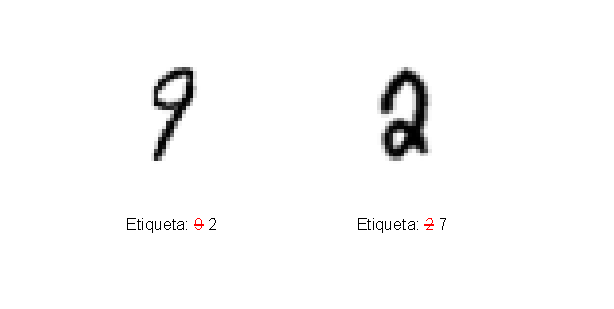
\includegraphics[width=0.8\textwidth]{figuras/labelflipping.pdf}
    \caption{Ejemplo de ataque \textit{random label flipping} en el conjunto de datos EMNIST. Las etiquetas de las muestras son cambiadas por una nueva etiqueta aleatoria manteniendo la muestra original. Fuente: Elaboración propia.}
    \label{fig:enter-label}
\end{figure}

\subsection{Ataques \textit{backdoor} basado en patrones}
También realizamos un ataque de \textit{backdoor} basado en patrones, en el que todos los clientes conocen el patrón completo y lo usan en su proceso de entrenamiento. Establecemos una etiqueta objetivo y un patrón. El número de tareas de \textit{backdoor} es el número de clientes adversarios. Con el fin de demostrar que el comportamiento observado no depende del patrón usado, usamos dos patrones: (1) un píxel blanco en la esquina inferior izquierda para EMNIST y Fashion MNIST o un cuadrado blanco de 5x5 en CIFAR-10, y (2) una cruz blanca de longitud 3 para EMNIST y Fashion MNIST y de longitud 5 para CIFAR-10. La diferencia de tamaño en los patrones se debe al uso del modelo de \textit{EfficientNet} pues este usa un recorte central en la imagen. Se pueden ver los patrones en la Figura \ref{fig:patterns}.

\begin{figure}[h!]
\centering
\begin{subfigure}{.16\linewidth}
  \centering
  
\includegraphics[width=0.8\linewidth]{figuras/backdoor/emnist.png}
  \caption{Imagen.}
  %\label{fig:sfig1}
\end{subfigure}
\begin{subfigure}{.16\linewidth}
  \centering
  
\includegraphics[width=0.8\linewidth]{figuras/backdoor/emnist_cross.png}
  \caption{Cruz.}
  %\label{fig:sfig2}
\end{subfigure}
\begin{subfigure}{.16\linewidth}
  \centering
  
\includegraphics[width=0.8\linewidth]{figuras/backdoor/emnist_square.png}
  \caption{Cuadrado.}
  %\label{fig:sfig3}
\end{subfigure}
\vskip\baselineskip
\begin{subfigure}{.16\linewidth}
  \centering
  
\includegraphics[width=0.8\linewidth]{figuras/backdoor/fashion.png}
  \caption{Imagen.}
  %\label{fig:sfig4}
\end{subfigure}
\begin{subfigure}{.16\linewidth}
  \centering
  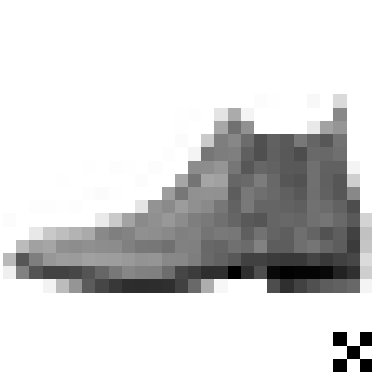
\includegraphics[width=0.8\linewidth]{figuras/backdoor/fashion_cross.png}
  \caption{Cruz.}
  %\label{fig:sfig5}
\end{subfigure}
\begin{subfigure}{.16\linewidth}
  \centering
  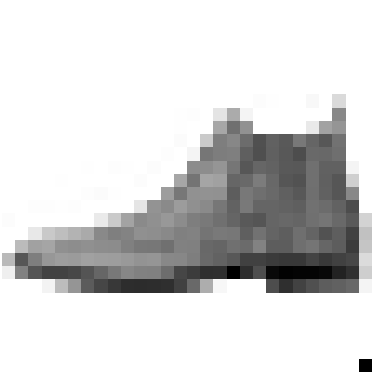
\includegraphics[width=0.8\linewidth]{figuras/backdoor/fashion_square.png}
  \caption{Cuadrado.}
  %\label{fig:sfig6}
\end{subfigure}
\vskip\baselineskip
\begin{subfigure}{.16\linewidth}
  \centering
  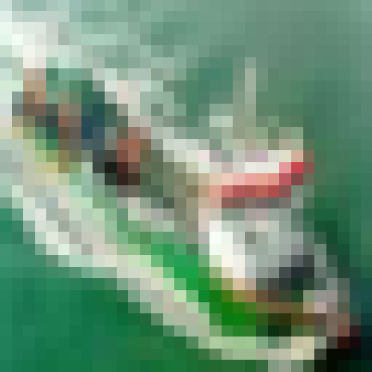
\includegraphics[width=0.8\linewidth]{figuras/backdoor/cifar.png}
  \caption{Imagen.}
  %\label{fig:sfig4}
\end{subfigure}
\begin{subfigure}{.16\linewidth}
  \centering
  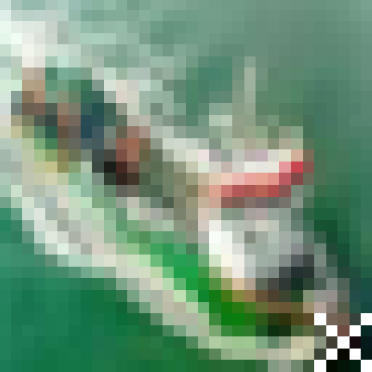
\includegraphics[width=0.8\linewidth]{figuras/backdoor/cifar_cross.png}
  \caption{Cruz.}
  %\label{fig:sfig5}
\end{subfigure}
\begin{subfigure}{.16\linewidth}
  \centering
  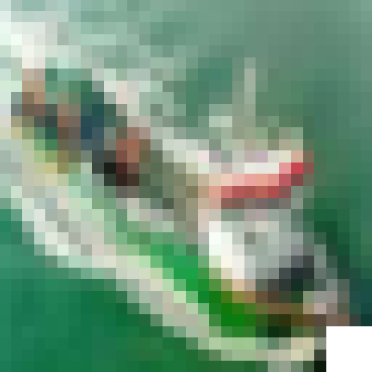
\includegraphics[width=0.8\linewidth]{figuras/backdoor/cifar_square.png}
  \caption{Cuadrado.}
  %\label{fig:sfig6}
\end{subfigure}
\vskip\baselineskip
\caption{Ejemplos de muestras originales (a, d y g) y envenenadas con patrón de cruz (b, e y h), y de cuadrado (c, f and i) en los conjuntos de datos
EMNIST, Fashion-MNIST y CIFAR, respectivamente.}
\label{fig:patterns}
\end{figure}

\section{Escenarios de los ataques}\label{sec:escenarios}
Con el objetivo de poner a prueba nuestras propuestas en distintos entornos consideramos dos escenarios distintos:
\begin{enumerate}
    \item \textbf{Escenario A:} Solo hay un único cliente adversario participando en una ronda de aprendizaje $t$.
    \item \textbf{Escenario B:} La cantidad de clientes adversarios en una ronda de aprendizaje se establece a la cantidad de mineros en la red. En el caso de que la arquitectura a comprobar haga uso de \textit{pooled-mining}, esto es, a cada minero se le asigna un subconjunto de los clientes y no hace uso de ningún tipo de recurso del subconjunto de otro minero, nos aseguramos que cada subconjunto contenga un cliente adversario.
\end{enumerate}

\section{Métricas usadas para la evaluación}\label{sec:metricas}
Consideraremos las métricas según el escenario que estemos cubriendo:

\subsection{Métricas en el caso sin atacantes}
En esta situación nos encontramos ante un caso genérico de clasificación de imágenes. Por lo tanto, usaremos la precisión o \textit{accuracy} en el conjunto de test de nuestro conjunto de datos para medir el rendimiento del modelo.

\subsection{Métricas para ataques bizantinos}
Cuando medimos una defensa contra un ataque bizantino, el objetivo es obtener el mejor rendimiento del modelo en la tarea planteada. Es por ello que comprobamos la precisión o \textit{accuracy} del modelo en el subconjunto de test del conjunto de datos que estamos considerando. Claramente, cuanto mayor sea este valor, mejor será la defensa contra este tipo de ataques.

\subsection{Métricas para ataques de backdoor}
A la hora de defendernos de un ataque de \textit{backdoor}, debemos de considerar dos aspectos distintos. Estos son, el rendimiento del modelo resultante en la tarea original y en la tarea inyectada. La meta es reducir el impacto del ataque lo máximo posible sin comprometer el rendimiento del modelo en la tarea original. Para ello consideramos dos conjuntos de test:
\begin{enumerate}
    \item \textbf{Conjunto de test original}. El conjunto de test original usado para medir el rendimiento en términos de la precisión o \textit{accuracy} en la tarea original.
    \item \textbf{Conjunto de test de \textit{backdoor}}. Este conjunto representa el ataque con el fin de medir el rendimiento de la tarea de \textit{backdoor}. Consiste del conjunto de test original pero envenenado usando el patrón, con el fin de medir la capacidad de generalización del ataque. 
\end{enumerate}

Una defensa será más efectiva cuanto más consiga prevenir el ataque (menor rendimiento en el test de \textit{backdoor}) minimizando la pérdida de rendimiento en la tarea original (mayor rendimiento en el test original).

Dado que los resultados pueden ser altamente heterogéneos en cada ronda de aprendizaje y con el fin de mostrar resultados robustos, mostramos tanto la métrica de la última ronda (\textit{accuracy}) como la media de cada una de estas métricas en las últimas diez rondas de aprendizaje ($accuracy_{10}$). Además, dado que los resultados entre mineros de una misma red pueden diferir en el caso de \ac{PoFL} y \ac{KFC}, mostramos las métricas del mejor minero en términos del rendimiento en la tarea original la cual se supone que puede ser medida en un caso real mediante el conjunto de validación usado en estas arquitecturas.

\section{Arquitecturas de referencia}
Comparamos \ac{KFC} y \ac{PoFL} con las siguientes arquitecturas de \ac{FL}, que representan las referencias clásicas y más estudiadas para \textit{blockchain} aplicado al \ac{FL}:
\begin{enumerate}
    \item \textbf{Cliente-Servidor (C-S)}. No hace ningún uso de \textit{blockchain}. Es uno de los escenarios de \ac{FL} más comunes donde un servidor central actúa como agregador y organiza todo el proceso de aprendizaje.
    \item \textbf{\textit{Proof of Work}}. El mecanismo de consenso donde los mineros compiten en una carrera computacional para resolver un puzzle. El ganador actúa como el agregador para una ronda dada. Consiste en un modelo desacoplado.
    \item \textbf{\textit{Proof of Stake}}. Una arquitectura similar a la anterior pero donde se decide usar \ac{PoS} como mecanismo de consenso como alternativa más eficiente a nivel energético para la red. Consiste en un modelo desacoplado.
\end{enumerate}

En todas las arquitecturas de referencia anteriores y en \ac{PoFL} usamos \ac{FedAvg}~\cite{mcmahan-2023} como el operador de agregación el cual es muchas veces considerado el operador de agregación por defecto para \ac{FL} y el más estudiado en la literatura. Además, dado que \ac{PoW} y \ac{PoS} utilizan la misma arquitectura \textit{blockchain} subyacente hemos decidido combinar los resultados de ambos con el fin de obtener una mayor comprensión y que llamaremos PoW/S.

\section{Detalles de implementación}
Los experimentos han sido realizados usando el framework de simulación de \ac{FL} \texttt{flex}~\cite{flex} y la librería de \ac{AA} \texttt{pytorch}~\cite{pytorch}. Con el fin de simular el comportamiento de una \textit{blockchain} en un escenario federado se ha implementado una librería compañera a \texttt{flex} llamada \texttt{flex-block}~\cite{flex}\footnote{\url{https://github.com/FLEXible-FL/flex-block}}. Además, se adjunta el código realizado\footnote{\url{https://github.com/mariogmarq/kfc-experiments}} para asegurar la reproducibilidad de los experimentos realizados.

 \chapter{Análisis de los resultados}\label{sec:resultados}

En esta sección se exponen los resultados de los experimentos explicados en la Sección~\ref{sec:experimentos}. En primer lugar, en la Sección \ref{sec:hipotesis} analizamos el funcionamiento de \ac{PoFL} como mecanismo de defensa. De las debilidades detectadas en esta sección surge \ac{KFC}, cuyo rendimiento como defensa analizamos, de forma comparativa con la propuesta anterior, en la sección \ref{sec:kfc_experiments}. 

\section{Análisis de PoFL como mecanismo de defensa}\label{sec:hipotesis}

A continuación veremos el rendimiento de \ac{PoFL} tanto en el caso en el que no hay ningún atacante en la red (vea Sección \ref{sec:sin_attack_pofl}) como en los escenarios A (vea Sección \ref{sec:pofl_a}) y B (vea Sección \ref{sec:pofl_b}).

\subsection{Rendimiento sin atacantes}\label{sec:sin_attack_pofl}
Al considerar el caso de que no haya ningún atacante en la red podemos observar tanto en la Tabla \ref{tab:baseline_pofl} como en la Figura \ref{fig:pofl_no_attacks} que tanto nuestra arquitecturas de referencia como aquella basada en \ac{PoFL} obtienen un rendimiento en términos de precisión
similar en todos los conjuntos de datos. Esto nos muestra que \ac{PoFL} es una buena arquitectura para el aprendizaje y una buena alternativa a nuestras arquitecturas de referencia. Esto indica que seleccionar únicamente un modelo basándose en un criterio de eficiencia en un conjunto de validación obtiene resultados similares a los de considerar todas las actualizaciones posibles.

\begin{table*}[!ht]
\centering
\begin{tabular}{lrrrrrr}
\toprule
 & \multicolumn{3}{c}{\textit{accuracy}} & \multicolumn{3}{c}{\textit{$accuracy_{10}$}}   \\
\toprule
       & \textbf{C-S} & \textbf{PoW/S} & \textbf{PoFL} & \textbf{C-S} & \textbf{PoW/S} & \textbf{PoFL}  \\ 
\toprule
\textbf{EMNIST} & 0.9810& \textbf{0.9924}& 0.9869& 0.9805& \textbf{0.9924}& 0.9845\\  
\midrule
\textbf{Fashion MNIST}& 0.9030& \textbf{0.9033}& 0.8972& \textbf{0.9041}& 0.9040& 0.8973\\ 
\midrule
\textbf{CIFAR-10}        & \textbf{0.9688}& 0.9677& 0.9569& \textbf{0.9686}& 0.9676& 0.9564\\
\bottomrule
\end{tabular}
\caption{\textit{accuracy} y \textit{$accuracy_{10}$} comparando PoFL con las arquitecturas de referencia sin ningún atacante.}\label{tab:baseline_pofl}

\end{table*}
\begin{figure}[!ht]
\begin{subfigure}{0.49\linewidth}
  \centering
  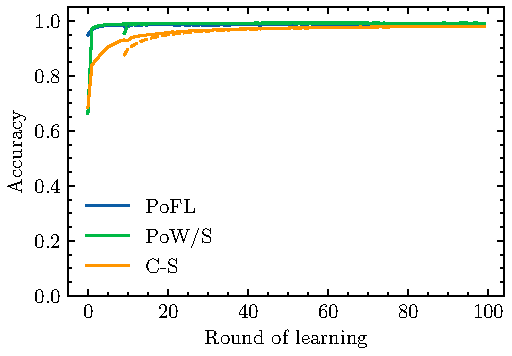
\includegraphics[width=\linewidth]{figuras/graficas/baseline_mnist_one.pdf}
  \caption{EMNIST.}
  %\label{fig:sfig1}
\end{subfigure} 
\begin{subfigure}{0.49\linewidth}
  \centering
  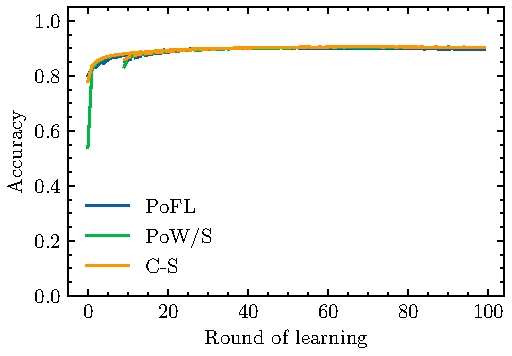
\includegraphics[width=\linewidth]{figuras/graficas/baseline_fashion_one.pdf}
  \caption{Fashion MNIST.}
  %\label{fig:sfig3}
\end{subfigure} 
\vskip\baselineskip
\centering
\begin{subfigure}{0.49\linewidth}
  \centering
  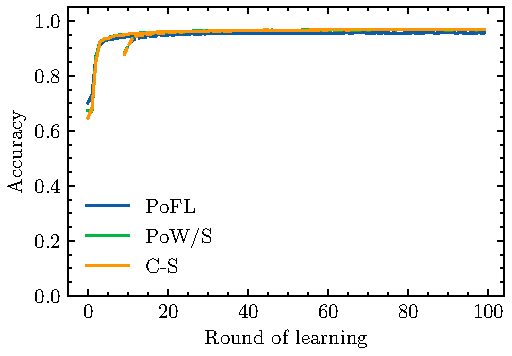
\includegraphics[width=\linewidth]{figuras/graficas/baseline_cifar_one.pdf}
  \caption{CIFAR.}
  %\label{fig:sfig2}
\end{subfigure}
\vskip\baselineskip
\caption{$accuracy$ (línea) y $accuracy_{10}$ (línea discontinua) de las tareas originales  EMNIST (a), Fashion MNIST (b) y CIFAR (c), sin ningún atacante presente.}
\label{fig:pofl_no_attacks}
\end{figure}


\newpage
\subsection{Escenario A: Un solo atacante}\label{sec:pofl_a}
En esta sección analizamos el rendimiento de \ac{PoFL} en el \textbf{escenario A}. Analizando los resultados expuestos en las Tablas \ref{tab:poflbackdoor_a} y \ref{tab:poflbyzantine_a} junto a las Figuras \ref{fig:pofl_a_backdoor} y \ref{fig:pofl_byzantine_a}, aunque se abarcan diferentes tipos de ataques, se puede observar las siguientes conclusiones comunes:

\begin{itemize}
	\item \ac{PoFL} demuestra una superioridad en rendimiento en todos los conjuntos de datos bajo ambos ataques, obteniendo la mayor precisión durante todo el proceso de entrenamiento. Además los resultados logrados por \ac{PoFL} son similares a los obtenidos para el caso donde no considerábamos atacantes, resaltando así su capacidad como mecanismo de defensa.

    \item Para nuestra tarea de \textit{backdoor}, representada en la Tabla \ref{tab:poflbackdoor_a} y Figura \ref{fig:pofl_a_backdoor}, \ac{PoFL} logra mitigar el ataque obteniendo una precisión mínima que nos sugiere la exitosa supresión de la tarea inyectada. Además, \ac{PoFL} además de mitigar el ataque consigue mantener un buen rendimiento en la tarea original, asegurando tanto la mitigación de ataques como el objetivo original. Por otra parte, nuestras arquitecturas de referencia no ofrecen ningún tipo de resistencia obteniendo una precisión casi perfecta en la tarea secundaria.

    \item Si observamos el ataque bizantino, cuyos resultados aparecen en la Tabla \ref{tab:poflbyzantine_a} y Figura \ref{fig:pofl_byzantine_a}, vemos como \ac{PoFL} vuelve a obtener los mismos resultados mientras que nuestras arquitecturas de referencia ven cómo su rendimiento es degradado presentando además múltiples perturbaciones en las medidas.
\end{itemize}

\begin{table*}[!ht]
\centering
\begin{tabular}{llrrrrrr}
\toprule
 & & \multicolumn{3}{c}{\textit{accuracy}} & \multicolumn{3}{c}{\textit{$accuracy_{10}$}}   \\
\toprule
       &          & \textbf{C-S} & \textbf{PoW/S} & \textbf{PoFL} & \textbf{C-S} & \textbf{PoW/S} & \textbf{PoFL}  \\ 
\toprule
\textbf{EMNIST} & Original & 0.9821        & 0.9793  & \textbf{0.9930}  & 0.9825        & 0.9809  & \textbf{0.9930}   \\  
       & Backdoor & 0.9999        & 0.9994  & \textbf{0.0980} & 0.9997        & 0.9996  & \textbf{0.0979}   \\  
\midrule
\textbf{Fashion}   & Original & 0.8462        & 0.8414  & \textbf{0.8961}  & 0.8416        & 0.8486  & \textbf{0.8986}  \\ 
 \textbf{MNIST}    & Backdoor & 0.9955        & 0.9969  & \textbf{0.0871}& 0.9884        & 0.9878  & \textbf{0.0989}   \\ 
\midrule
\textbf{CIFAR-10}        & Original & 0.9103        & 0.9038  & \textbf{0.9397}  & 0.9021        & 0.8762  & \textbf{0.9283}   \\ 
                & Backdoor & 0.9676        & 0.9704  & \textbf{0.1163}   & 0.9348        & 0.9736  & \textbf{0.0849}  \\ 
\bottomrule
\end{tabular}
\caption{\textit{accuracy} y \textit{$accuracy_{10}$} comparando PoFL con las arquitecturas de referencia en el \textbf{escenario A} ante un ataque de backdoor.}\label{tab:poflbackdoor_a}
\end{table*}

\begin{figure}[!ht]
\begin{subfigure}{0.49\linewidth}
  \centering
  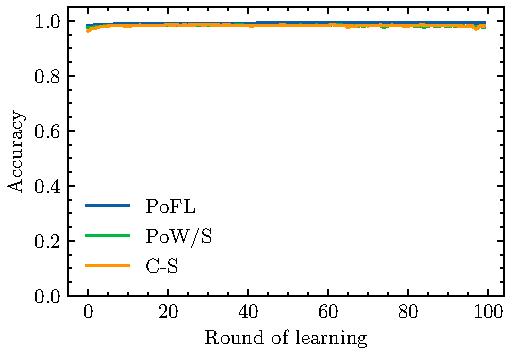
\includegraphics[width=\linewidth]{figuras/graficas/original_mnist_one.pdf}
  \caption{EMNIST (Tarea original).}
  %\label{fig:sfig1}
\end{subfigure} 
\begin{subfigure}{0.49\linewidth}
  \centering
  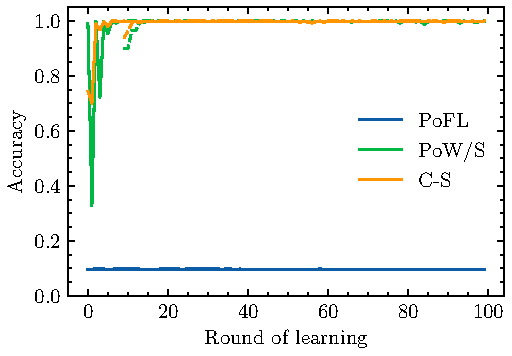
\includegraphics[width=\linewidth]{figuras/graficas/backdoor_mnist_one.pdf}
  \caption{EMNIST (Tarea backdoor).}
  %\label{fig:sfig1}
\end{subfigure} 
\vskip\baselineskip
\begin{subfigure}{0.49\linewidth}
  \centering
  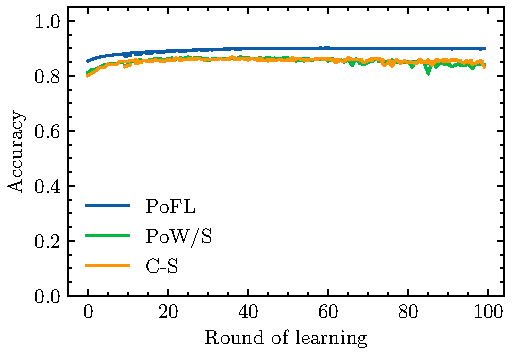
\includegraphics[width=\linewidth]{figuras/graficas/original_fashion_one.pdf}
  \caption{Fashion EMNIST (Tarea original).}
  %\label{fig:sfig3}
\end{subfigure} 
\begin{subfigure}{0.49\linewidth}
  \centering
  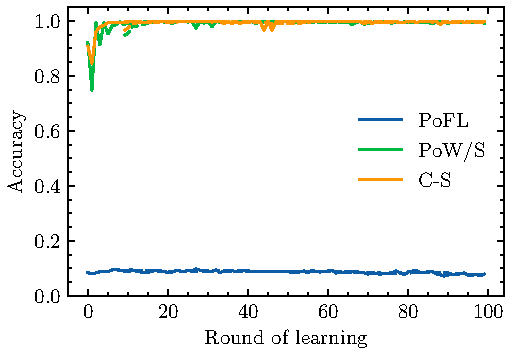
\includegraphics[width=\linewidth]{figuras/graficas/backdoor_fashion_one.pdf}
  \caption{Fashion EMNIST (Tarea backdoor).}
  %\label{fig:sfig2}
\end{subfigure}
\vskip\baselineskip
\begin{subfigure}{0.49\linewidth}
  \centering
  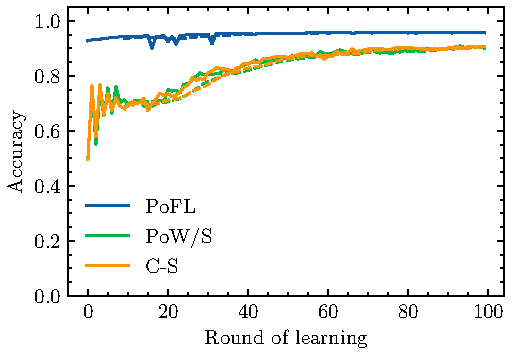
\includegraphics[width=\linewidth]{figuras/graficas/original_cifar_one.pdf}
  \caption{CIFAR (Tarea original).}
  %\label{fig:sfig2}
\end{subfigure}
\begin{subfigure}{0.49\linewidth}
  \centering
  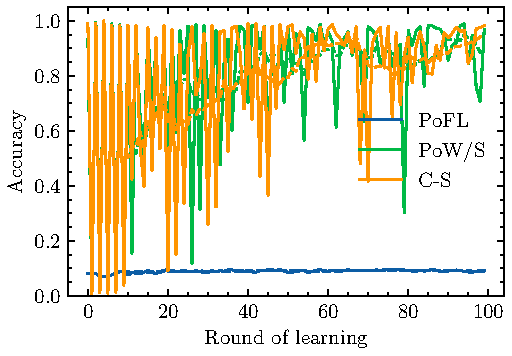
\includegraphics[width=\linewidth]{figuras/graficas/backdoor_cifar_one.pdf}
  \caption{CIFAR (Tarea backdoor).}
  %\label{fig:sfig4}
\end{subfigure}
\vskip\baselineskip
\caption{$accuracy$ (línea) y $accuracy_{10}$ (línea discontinua) de las tareas originales y backdoor en EMNIST (a y b), Fashion MNIST (c y d) y CIFAR (e y f), respectivamente, en el \textbf{escenario A}.}
\label{fig:pofl_a_backdoor}
\end{figure}

Basándonos en estas observaciones, los resultados experimentales ofrecen pruebas convincentes de que \ac{PoFL} constituye una arquitectura de \textit{blockchain} aplicada a \ac{FL} robusta contra ataques de \textit{backdoor} y bizantinos dentro del escenario investigado. Estos hallazgos confirman que el mecanismo de consenso basado en el rendimiento empleado por \textit{PoFL}, junto con la arquitectura de \textit{pooled-mining}, filtra de manera eficaz las actualizaciones maliciosas inyectadas por clientes adversarios debido a que estos tienden a crear actualizaciones con mala calidad.

\begin{table*}[!ht]
\centering
\begin{tabular}{lrrrrrr}
\toprule
 & \multicolumn{3}{c}{\textit{accuracy}} & \multicolumn{3}{c}{\textit{$accuracy_{10}$}}   \\
\toprule
       & \textbf{C-S} & \textbf{PoW/S} & \textbf{PoFL} & \textbf{C-S} & \textbf{PoW/S} & \textbf{PoFL}  \\ 
\toprule
\textbf{EMNIST} & 0.8931& 0.1000& \textbf{0.9926}& 0.6594& 0.1030& \textbf{0.9925}\\  
\midrule
\textbf{Fashion MNIST}& 0.8264& 0.1041& \textbf{0.9051}& 0.8363& 0.0978& \textbf{0.9049}\\ 
\midrule
\textbf{CIFAR-10}        & 0.2868& 0.6870& \textbf{0.9628}& 0.4196& 0.6685& \textbf{0.9604}\\
\bottomrule
\end{tabular}
\caption{\textit{accuracy} y \textit{$accuracy_{10}$} comparando PoFL con las arquitecturas de referencia en el \textbf{escenario A} ante un ataque bizantino.}\label{tab:poflbyzantine_a}

\end{table*}


\begin{figure}[!ht]
\begin{subfigure}{0.49\linewidth}
  \centering
  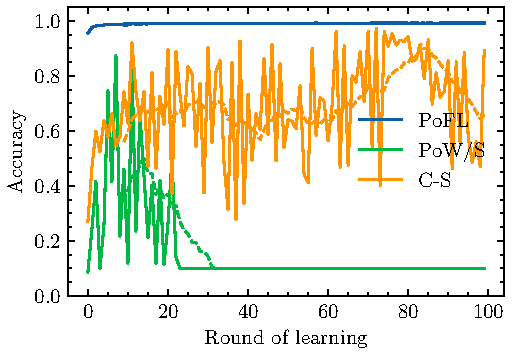
\includegraphics[width=\linewidth]{figuras/graficas/byzantine_mnist_one.pdf}
  \caption{EMNIST.}
  %\label{fig:sfig1}
\end{subfigure} 
\begin{subfigure}{0.49\linewidth}
  \centering
  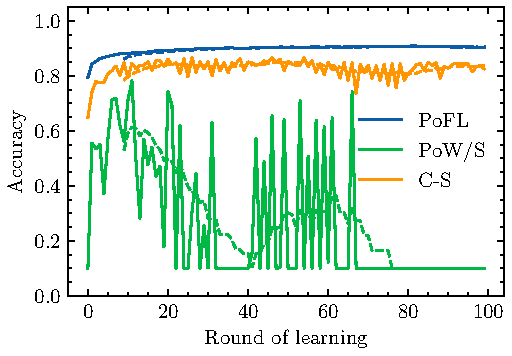
\includegraphics[width=\linewidth]{figuras/graficas/byzantine_fashion_one.pdf}
  \caption{Fashion EMNIST.}
  %\label{fig:sfig3}
\end{subfigure} 
\vskip\baselineskip
\centering
\begin{subfigure}{0.49\linewidth}
  \centering
  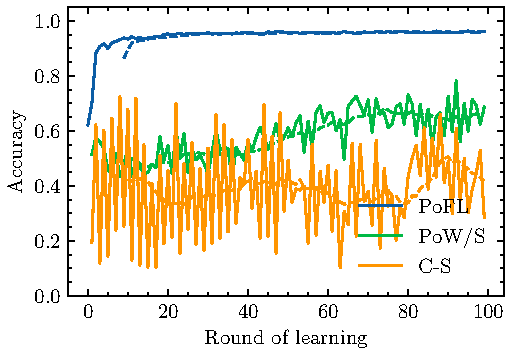
\includegraphics[width=\linewidth]{figuras/graficas/byzantine_cifar_one.pdf}
  \caption{CIFAR.}
  %\label{fig:sfig2}
\end{subfigure}
\vskip\baselineskip
\caption{$accuracy$ (línea) y $accuracy_{10}$ (línea discontinua) de las tareas originales  EMNIST (a), Fashion MNIST (b) y CIFAR (c), bajo un ataque bizantino en el \textbf{escenario A}.}
\label{fig:pofl_byzantine_a}
\end{figure}

\newpage
\subsection{Escenario B: Todos los mineros son atacados}\label{sec:pofl_b}
A continuación estudiamos el rendimiento de \ac{PoFL} como defensa en el \textbf{escenario B}. Los resultados han sido representados tanto en las Tablas \ref{tab:poflbackdoor_b} y \ref{tab:poflbyzantine_b} como en las Figuras \ref{fig:pofl_b_backdoor} y \ref{fig:pofl_byzantine_b}. Tras su observación llegamos a las siguientes conclusiones:
\begin{itemize}
	\item A diferencia del escenario anterior, donde \ac{PoFL} aparecía como la arquitectura con mayor rendimiento, en este caso exhibe el peor rendimiento en la mayoría de las tareas. En todas ellas muestra un comportamiento inconsistente con grandes fluctuaciones durante todo el proceso de entrenamiento. Nuestras arquitecturas de referencia, sin embargo, mantienen una precisión similar en todas las pruebas en comparación con el escenario anterior.
	
	\item En la tarea de \textit{backdoor}, acudiendo a la Tabla \ref{tab:poflbackdoor_b} y Figura \ref{fig:pofl_b_backdoor}, vemos como \ac{PoFL} tiene el peor rendimiento en la tarea original en los tres conjuntos. Además, aunque inferior a las arquitecturas de referencia, \ac{PoFL} muestra un alto rendimiento en la tarea secundaria indicando el éxito del ataque de \textit{backdoor} bajo estas circunstancias.
	
	\item Respecto al ataque bizantino, observando la Tabla \ref{tab:poflbyzantine_b} y Figura \ref{fig:pofl_byzantine_b}, vemos que el rendimiento de \ac{PoFL} es similar al de las arquitecturas de referencia, denotando ser vulnerable ante este tipo de ataques.
\end{itemize}


\begin{table}

    \centering
    \begin{tabular}{llcccccc}
    	\toprule
           &&\multicolumn{3}{c}{\textit{accuracy}}&  \multicolumn{3}{c}{\textit{$accuracy_{10}$}}\\
           \toprule
           &&\textbf{C-S} &  \textbf{PoW/S} &  \textbf{PoFL} &  \textbf{C-S} &  \textbf{PoW/S} & \textbf{PoFL} 
\\
\toprule
           \textbf{EMNIST} &Original 
&0.9863        &  \textbf{0.9889}  &  0.8986&  0.9866        &  0.9888  & \textbf{0.9108} 
\\
           &Backdoor 
&0.9999        &  1.0000     &  \textbf{0.7536}   &  0.9997        &  1.0000     & \textbf{0.8002} 
\\
\midrule
           \textbf{Fashion}   &Original 
&0.8593        &  \textbf{0.8729}  &  0.8133    &  0.9997        &  1.0000     & \textbf{0.8002} 
\\
           \textbf{MNIST}    &Backdoor 
&0.9955        &  0.9977  &  \textbf{0.8199} &  0.9891        &  0.9963  & \textbf{0.9181}
\\
\midrule
           \textbf{CIFAR-10}        &Original 
&0.9101        &  \textbf{0.9436}  &  0.8485  &  0.9032        &  \textbf{0.9402}  & 0.8223 
\\
           &Backdoor &0.9676        &  0.9922  &  \textbf{0.8535}   &  0.9837        &  0.9928  & \textbf{0.9151} \\
           \bottomrule
    \end{tabular}
    \caption{\textit{accuracy} y \textit{$accuracy_{10}$} comparando PoFL con las arquitecturas de referencia en el \textbf{escenario B} ante un ataque de backdoor.}\label{tab:poflbackdoor_b}
\end{table}


\begin{figure}[h!]
\begin{subfigure}{0.49\linewidth}
  \centering
  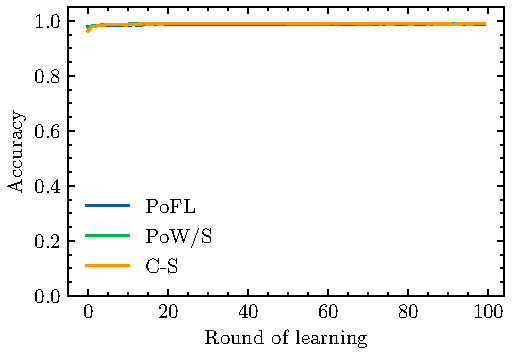
\includegraphics[width=\linewidth]{figuras/graficas/original_mnist_all.pdf}
  \caption{EMNIST (Tarea original).}
  %\label{fig:sfig1}
\end{subfigure} 
\begin{subfigure}{0.49\linewidth}
  \centering
  \includegraphics[width=\linewidth]{figuras/graficas/backdoor_mnist_all.pdf}
  \caption{EMNIST (Tarea backdoor).}
  %\label{fig:sfig1}
\end{subfigure} 
\vskip\baselineskip
\begin{subfigure}{0.49\linewidth}
  \centering
  \includegraphics[width=\linewidth]{figuras/graficas/original_fashion_all.pdf}
  \caption{Fashion EMNIST (Tarea original).}
  %\label{fig:sfig3}
\end{subfigure} 
\begin{subfigure}{0.49\linewidth}
  \centering
  \includegraphics[width=\linewidth]{figuras/graficas/backdoor_fashion_all.pdf}
  \caption{Fashion EMNIST (Tarea backdoor).}
  %\label{fig:sfig2}
\end{subfigure}
\vskip\baselineskip
\begin{subfigure}{0.49\linewidth}
  \centering
  \includegraphics[width=\linewidth]{figuras/graficas/original_cifar_all.pdf}
  \caption{CIFAR (Tarea original).}
  %\label{fig:sfig2}
\end{subfigure}
\begin{subfigure}{0.49\linewidth}
  \centering
  \includegraphics[width=\linewidth]{figuras/graficas/backdoor_cifar_all.pdf}
  \caption{CIFAR (Tarea backdoor).}
  %\label{fig:sfig4}
\end{subfigure}
\vskip\baselineskip
\caption{$accuracy$ (línea) y $accuracy_{10}$ (línea discontinua) de las tareas originales y backdoor en EMNIST (a y b), Fashion MNIST (c y d) y CIFAR (e y f), respectivamente, en el \textbf{escenario B}.}
\label{fig:pofl_b_backdoor}
\end{figure}
\begin{table}
    \centering
    \begin{tabular}{lcccccc}
    	\toprule
           &\multicolumn{3}{c}{\textit{accuracy}}&  \multicolumn{3}{c}{\textit{$accuracy_{10}$}}\\
           \toprule
           &\textbf{C-S} &  \textbf{PoW/S} &  \textbf{PoFL} &  \textbf{C-S} &  \textbf{PoW/S} & \textbf{PoFL} 
\\
\toprule
           \textbf{EMNIST} &\textbf{0.9232}&  0.7351&  0.9202&  0.7770&  0.7246& \textbf{0.9120}\\
           \midrule
           \textbf{Fashion MNIST}&\textbf{0.8329}&  0.7372&  0.7344&  \textbf{0.8222}&  0.8087& 0.7476\\
           \midrule
           \textbf{CIFAR-10}        &0.6168&  \textbf{0.7967}&  0.5648&  0.6692&  \textbf{0.7545}& 0.5648\\
           \bottomrule
    \end{tabular}
    \caption{\textit{accuracy} y \textit{$accuracy_{10}$} comparando PoFL con las arquitecturas de referencia en el \textbf{escenario B} ante un ataque de bizantino.}\label{tab:poflbyzantine_b}

\end{table}
\begin{figure}[!ht]
\begin{subfigure}{0.49\linewidth}
  \centering
  \includegraphics[width=\linewidth]{figuras/graficas/byzantine_mnist_all.pdf}
  \caption{EMNIST.}
  %\label{fig:sfig1}
\end{subfigure} 
\begin{subfigure}{0.49\linewidth}
  \centering
  \includegraphics[width=\linewidth]{figuras/graficas/byzantine_fashion_all.pdf}
  \caption{Fashion EMNIST.}
  %\label{fig:sfig3}
\end{subfigure} 
\vskip\baselineskip
\centering
\begin{subfigure}{0.49\linewidth}
  \centering
  \includegraphics[width=\linewidth]{figuras/graficas/byzantine_cifar_all.pdf}
  \caption{CIFAR.}
  %\label{fig:sfig2}
\end{subfigure}
\vskip\baselineskip
\caption{$accuracy$ (línea) y $accuracy_{10}$ (línea discontinua) de las tareas originales  EMNIST (a), Fashion MNIST (b) y CIFAR (c), bajo un ataque bizantino en el \textbf{escenario B}.}
\label{fig:pofl_byzantine_b}
\end{figure}

En conclusión, los experimentos muestran un panorama preocupante sobre la idoneidad de \ac{PoFL} en este escenario. Como se ha demostrado en las observaciones anteriores, \ac{PoFL} exhibe una vulnerabilidad significativa a los ataques de \textit{backdoor}. No solo logra una precisión preocupantemente alta en las tareas de \textit{backdoor} en promedio, sino que su rendimiento en la tarea original también sufre un detrimento sustancial. Además, muestra un deterioro grave ante ataques bizantinos, obteniendo resultados similares a aquellos obtenidos por nuestras arquitecturas de referencia. Esto se debe a que cuando el rendimiento de todas las \textit{pools} se ve comprometido, el mecanismo de consenso es incapaz de filtrar las actualizaciones maliciosas.

Esta vulnerabilidad de \ac{PoFL} motiva el diseño de \ac{KFC}, como la combinación de \ac{PoFL} y un mecanismo de defensa en cada minero, lo que lo hace resistente a ataques adversarios incluso cuando todos los mineros están siendo atacados. Abordamos esta cuestión en la siguiente sección.


\newpage
\section{Análisis de rendimiento de KFC}\label{sec:kfc_experiments}
En esta sección analizaremos los resultados de \ac{KFC} en los escenarios A (vea Sección \ref{sec:kfc_a}) y B (vea Sección \ref{sec:kfc_b}). Además, los compararemos con aquellos de \ac{PoFL} obtenidos en la Sección \ref{sec:hipotesis}.

\subsection{Escenario A: Un solo atacante}\label{sec:kfc_a}

Primero nos centraremos en el \textbf{escenario A} donde \ac{PoFL} ya se mostraba como una defensa válida. Los resultados expuestos en las Tablas \ref{tab:kfcbackdoor_a} y \ref{tab:kfcbyzantine_a} junto a las Figuras \ref{fig:kfc_a} y \ref{fig:kfc_byzantine_a}, nos indican que \ac{KFC} también es una defensa eficaz para ambos tipos de ataques. Si observamos con detalle, vemos que el rendimiento de \ac{KFC} tanto en la tarea original del ataque de \textit{backdoor} como en el ataque bizantino es ligeramente inferior al de \ac{PoFL}. Esto es un resultado esperado y conocido del mecanismo de agregación Krum~\cite{krum-2017}, debido a seleccionar únicamente al cliente que minimiza la distancia geométrica, lo que causa una pérdida de precisión en la tarea original pero también en la tarea de \textit{backdoor}. Podemos concluir por tanto que \ac{KFC} se presenta en este escenario como una arquitectura viable para implementar \ac{FL} y \textit{blockchain} mientras ofrece una capa de seguridad, siendo igual de viable que \ac{PoFL} pues ambas tienen sus características.


\begin{table*}[h!]
\centering
\begin{tabular}{llrrrr}
\toprule
 & & \multicolumn{2}{c}{\textit{accuracy}} & \multicolumn{2}{c}{\textit{$accuracy_{10}$}}   \\
 \toprule
\textbf{}     &          & \textbf{PoFL}    & \textbf{KFC} & \textbf{PoFL}    & \textbf{KFC} \\ 
\midrule
\textbf{EMNIST}        & Original &   \textbf{0.9930}&  0.9889& \textbf{0.9930}& 0.9887 \\ 
              & Backdoor &     0.0980& \textbf{0.0964}&    0.0979&     \textbf{ 0.0970} \\ 
\midrule
\textbf{Fashion} & Original &    \textbf{0.8961}& 0.8645&  \textbf{0.8986}&   0.8645    \\ 
\textbf{MNIST}  & Backdoor &   0.0871& \textbf{0.0768}&  0.0989   &  \textbf{0.0813}    \\ 
\midrule
\textbf{CIFAR-10}      & Original & \textbf{0.9397}& 0.8870& \textbf{0.9283}& 0.8839\\ 
                        & Backdoor &  0.1163& \textbf{0.1025}& \textbf{0.0849}&  0.0981\\ 
\bottomrule
\end{tabular}
    \caption{\textit{accuracy} y \textit{$accuracy_{10}$} comparando PoFL y KFC en el \textbf{escenario A} ante un ataque de backdoor.} \label{tab:kfcbackdoor_a}

\end{table*}


\begin{figure}[h!]
\begin{subfigure}{0.49\linewidth}
  \centering
  \includegraphics[width=\linewidth]{figuras/graficas/kfc_vs_pofl_original_mnist_one.pdf}
  \caption{EMNIST (Tarea original).}
  %\label{fig:sfig1}
\end{subfigure} 
\begin{subfigure}{0.49\linewidth}
  \centering
  \includegraphics[width=\linewidth]{figuras/graficas/kfc_vs_pofl_backdoor_mnist_one.pdf}
  \caption{EMNIST (Tarea backdoor).}
  %\label{fig:sfig1}
\end{subfigure} 
\vskip\baselineskip
\begin{subfigure}{0.49\linewidth}
  \centering
  \includegraphics[width=\linewidth]{figuras/graficas/kfc_vs_pofl_original_fashion_one.pdf}
  \caption{Fashion EMNIST (Tarea original).}
  %\label{fig:sfig3}
\end{subfigure} 
\begin{subfigure}{0.49\linewidth}
  \centering
  \includegraphics[width=\linewidth]{figuras/graficas/kfc_vs_pofl_backdoor_fashion_one.pdf}
  \caption{Fashion EMNIST (Tarea backdoor).}
  %\label{fig:sfig2}
\end{subfigure}
\vskip\baselineskip
\begin{subfigure}{0.49\linewidth}
  \centering
  \includegraphics[width=\linewidth]{figuras/graficas/kfc_vs_pofl_original_cifar_one.pdf}
  \caption{CIFAR (Tarea original).}
  %\label{fig:sfig2}
\end{subfigure}
\begin{subfigure}{0.49\linewidth}
  \centering
  \includegraphics[width=\linewidth]{figuras/graficas/kfc_vs_pofl_backdoor_cifar_one.pdf}
  \caption{CIFAR (Tarea backdoor).}
  %\label{fig:sfig4}
\end{subfigure}
\vskip\baselineskip
\caption{$accuracy$ (linea) y $accuracy_{10}$ (linea discontinua) de la tarea original y backdoor en EMNIST (a y b), Fashion MNIST (c y d) y CIFAR (e y f), respectivamente, en el \textbf{escenario A}.}
\label{fig:kfc_a}
\end{figure}


\begin{table*}[h!]
\centering
\begin{tabular}{lrrrr}
\toprule
 & \multicolumn{2}{c}{\textit{accuracy}} & \multicolumn{2}{c}{\textit{$accuracy_{10}$}}   \\
 \toprule
\textbf{}     & \textbf{PoFL}    & \textbf{KFC} & \textbf{PoFL}    & \textbf{KFC} \\ 
\midrule
\textbf{EMNIST}        &   \textbf{0.9926}&  0.9882& \textbf{0.9925}& 0.9880\\ 
\midrule
\textbf{Fashion MNIST}&    \textbf{0.9051}& 0.8705&  \textbf{0.9049}&   0.8684\\ 
\midrule
\textbf{CIFAR-10}      & \textbf{0.9628}& 0.8901& \textbf{0.9604}& 0.8875\\
\bottomrule
\end{tabular}
    \caption{\textit{accuracy} y \textit{$accuracy_{10}$} comparando PoFL y KFC en el \textbf{escenario A} ante un ataque bizantino.}  \label{tab:kfcbyzantine_a}

\end{table*}


\begin{figure}[!ht]
\begin{subfigure}{0.49\linewidth}
  \centering
  \includegraphics[width=\linewidth]{figuras/graficas/kfc_vs_pofl_byzantine_mnist_one.pdf}
  \caption{EMNIST.}
  %\label{fig:sfig1}
\end{subfigure} 
\begin{subfigure}{0.49\linewidth}
  \centering
  \includegraphics[width=\linewidth]{figuras/graficas/kfc_vs_pofl_byzantine_fashion_one.pdf}
  \caption{Fashion EMNIST.}
  %\label{fig:sfig3}
\end{subfigure} 
\vskip\baselineskip
\centering
\begin{subfigure}{0.49\linewidth}
  \centering
  \includegraphics[width=\linewidth]{figuras/graficas/kfc_vs_pofl_byzantine_cifar_one.pdf}
  \caption{CIFAR.}
  %\label{fig:sfig2}
\end{subfigure}
\vskip\baselineskip
\caption{$accuracy$ (línea) y $accuracy_{10}$ (línea discontinua) de las tareas originales  EMNIST (a), Fashion MNIST (b) y CIFAR (c), bajo un ataque bizantino en el \textbf{escenario A}.}
\label{fig:kfc_byzantine_a}
\end{figure}


\subsection{Escenario B: Todos los mineros son atacados}\label{sec:kfc_b}

En esta sección volvemos al escenario más exigente en el que ya no se puede asumir la existencia de una \textit{pool} no siendo atacada. Los resultados de \ac{KFC} en este escenario se muestran en las Tablas \ref{tab:kfcbackdoorb} y \ref{tab:kfcbyzantine_b} y Figuras \ref{fig:kfc_b_backdoor} y \ref{fig:kfc_byzantine_b}. Un análisis detallado de los resultados nos lleva a las siguientes conclusiones comunes:

\begin{itemize}
	\item La capacidad de \ac{KFC} para mantener la precisión en la tarea original de \textit{backdoor} en comparación con \ac{PoFL} demuestra su resistencia en el nuevo escenario donde todos los mineros están bajo ataque.
    \item Al el contrario que \ac{PoFL}, \ac{KFC} demuestra una resistencia excepcional ante todos los ataques, logrando una precisión mínima en la tarea de \textit{backdoor} y mantener el rendimiento en el ataque bizantino, mitigando efectivamente los ataques.
\end{itemize}

En resumen, \ac{KFC} destaca como mecanismo de defensa. Los resultados nos indica como logra mitigar ambos tipos de ataques considerados, logrando reducir el impacto de la \textit{backdoor} mientras se observa un rendimiento alto en la tarea original y en el ataque de tipo bizantino, superando a \ac{PoFL} y nuestras arquitecturas de referencia en los entornos de la experimentación. Estos hallazgos confirman con firmeza que \ac{KFC} supera a \ac{PoFL} como la mejor opción en escenarios donde todas las \textit{pools} podrían estar comprometidas. \ac{KFC} logra eficazmente el doble objetivo de defender contra los ataques de \textit{backdoor} en \ac{FL}: maximizar el rendimiento de la tarea original y minimizar el impacto de la tarea inyectada. Además, su rendimiento contra ataques bizantinos se muestra excelente al presentar un comportamiento estable y una alta precisión. Esto se debe a que el mecanismo de agregación Krum permite filtrar actualizaciones maliciosas dentro de cada \textit{pool} y logrando así que el mecanismo de consenso basado en rendimiento ofrezca un modelo no comprometido.



\begin{table}
    \centering
    \begin{tabular}{llcccc}
    	\toprule
            &&\multicolumn{2}{c}{\textit{accuracy}}&  \multicolumn{2}{c}{\textit{$accuracy_{10}$}
}\\
\toprule
            &&\textbf{PoFL}    &  \textbf{KFC} &  & \textbf{KFC}
\\
\toprule
            \textbf{EMNIST}        &Original 
&0.8986  &  \textbf{0.9921}  &  0.9108 & \textbf{0.9922}    
\\
            &Backdoor 
&0.7536  &  \textbf{0.0995}   &  0.8002 & \textbf{0.0994}     
\\
\midrule
            \textbf{Fashion} &Original 
&0.8133 &  \textbf{0.9000}   &  0.8002 & \textbf{0.9000}    
\\
            \textbf{MNIST}  &Backdoor 
&0.8199  &  \textbf{0.0958}  &  0.9181 & \textbf{0.0894}    
\\
\midrule
            \textbf{CIFAR-10}      &Original 
&\textbf{0.8485}  &  0.8214  &  0.8223 & \textbf{0.9123}     
\\
            &Backdoor &0.8535  &  \textbf{0.1163}  &  0.9151 & \textbf{0.1016}    \\
\bottomrule
    \end{tabular}
     \caption{\textit{accuracy} y \textit{$accuracy_{10}$} comparando PoFL y KFC en el \textbf{escenario B} ante un ataque de backdoor.}
    \label{tab:kfcbackdoorb}
\end{table}

\begin{figure}[h!]
\begin{subfigure}{0.49\linewidth}
  \centering
  \includegraphics[width=\linewidth]{figuras/graficas/pofl_vs_kfc_original_mnist_all.pdf}
  \caption{EMNIST (Tarea original).}
  %\label{fig:sfig1}
\end{subfigure} 
\begin{subfigure}{0.49\linewidth}
  \centering
  \includegraphics[width=\linewidth]{figuras/graficas/pofl_vs_kfc_backdoor_mnist_all.pdf}
  \caption{EMNIST (Tarea backdoor).}
  %\label{fig:sfig1}
\end{subfigure} 
\vskip\baselineskip
\begin{subfigure}{0.49\linewidth}
  \centering
  \includegraphics[width=\linewidth]{figuras/graficas/pofl_vs_kfc_original_fashion_all.pdf}
  \caption{Fashion EMNIST (Tarea original).}
  %\label{fig:sfig3}
\end{subfigure} 
\begin{subfigure}{0.49\linewidth}
  \centering
  \includegraphics[width=\linewidth]{figuras/graficas/pofl_vs_kfc_backdoor_fashion_all.pdf}
  \caption{Fashion EMNIST (Tarea backdoor).}
  %\label{fig:sfig2}
\end{subfigure}
\vskip\baselineskip
\begin{subfigure}{0.49\linewidth}
  \centering
  \includegraphics[width=\linewidth]{figuras/graficas/pofl_vs_kfc_original_cifar_all.pdf}
  \caption{CIFAR (Tarea original).}
  %\label{fig:sfig2}
\end{subfigure}
\begin{subfigure}{0.49\linewidth}
  \centering
  \includegraphics[width=\linewidth]{figuras/graficas/pofl_vs_kfc_backdoor_cifar_all.pdf}
  \caption{CIFAR (Tarea backdoor).}
  %\label{fig:sfig4}
\end{subfigure}
\vskip\baselineskip
\caption{$accuracy$ (linea) y $accuracy_{10}$ (linea discontinua) de la tarea original y backdoor en EMNIST (a y b), Fashion MNIST (c y d) y CIFAR (e y f), respectivamente, en el \textbf{escenario B}.}
\label{fig:kfc_b_backdoor}
\end{figure}

\begin{table*}[h!]
\centering
\begin{tabular}{lrrrr}
\toprule
 & \multicolumn{2}{c}{\textit{accuracy}} & \multicolumn{2}{c}{\textit{$accuracy_{10}$}}   \\
 \toprule
\textbf{}     & \textbf{PoFL}    & \textbf{KFC} & \textbf{PoFL}    & \textbf{KFC} \\ 
\midrule
\textbf{EMNIST}        &   0.9202&  \textbf{0.9881}& 0.9120& \textbf{0.9881}\\ 
\midrule
\textbf{Fashion MNIST}&    0.7344& \textbf{0.8709}&  0.7476&   \textbf{0.8690}\\ 
\midrule
\textbf{CIFAR-10}      & 0.5681& \textbf{0.8856}& 0.5648& \textbf{0.8914}\\
\bottomrule
\end{tabular}
    \caption{\textit{accuracy} y \textit{$accuracy_{10}$} comparando PoFL y KFC en el \textbf{escenario B} ante un ataque bizantino.}  \label{tab:kfcbyzantine_b}

\end{table*}


\begin{figure}[!ht]
\begin{subfigure}{0.49\linewidth}
  \centering
  \includegraphics[width=\linewidth]{figuras/graficas/pofl_vs_kfc_byzantine_mnist_all.pdf}
  \caption{EMNIST.}
  %\label{fig:sfig1}
\end{subfigure} 
\begin{subfigure}{0.49\linewidth}
  \centering
  \includegraphics[width=\linewidth]{figuras/graficas/pofl_vs_kfc_byzantine_fashion_all.pdf}
  \caption{Fashion EMNIST.}
  %\label{fig:sfig3}
\end{subfigure} 
\vskip\baselineskip
\centering
\begin{subfigure}{0.49\linewidth}
  \centering
  \includegraphics[width=\linewidth]{figuras/graficas/pofl_vs_kfc_byzantine_cifar_all.pdf}
  \caption{CIFAR.}
  %\label{fig:sfig2}
\end{subfigure}
\vskip\baselineskip
\caption{$accuracy$ (línea) y $accuracy_{10}$ (línea discontinua) de las tareas originales  EMNIST (a), Fashion MNIST (b) y CIFAR (c), bajo un ataque bizantino en el \textbf{escenario B}.}
\label{fig:kfc_byzantine_b}
\end{figure}


\part{Conclusiones y trabajo futuro}

\chapter{Conclusiones}\label{sec:conclusiones}

En este capítulo se resumen las conclusiones principales del trabajo. Algunas de ellas darán lugar a posibles líneas de desarrollo de trabajo futuro.

En el contexto de los sistemas de \ac{IA}, la seguridad y la privacidad son aspectos fundamentales que no pueden ser subestimados. La creciente preocupación popular debido al creciente uso de estos sistemas ha llevado a la aparición del concepto de sistemas de \textit{Trustworthy AI} y  \textit{High-Risk AI Systems} por parte de organismos como la Unión Europea. Estos requisitos nos llevan a investigar maneras de garantizar la fiabilidad de los sistemas. Usualmente, aquellos sistemas de \ac{IA} que utilizan \ac{FL} manejan datos sensibles que, si no se protegen adecuadamente, pueden ser vulnerables a una variedad de ataques, incluyendo la filtración de datos privados y la manipulación maliciosa del modelo.

Es por ello que durante este trabajo nos hemos centrado en estudiar cómo la tecnología \textit{blockchain} puede ayudarnos a proteger un esquema federado. Se exponen a continuación los resultados observados:
\begin{itemize}
    \item Se ha observado cómo la combinación de las tecnologías \textit{blockchain} y \ac{FL} ayudan a resolver muchos problemas presentes en el paradigma de aprendizaje actual. Aunque hayamos hecho hincapié en aquellos relacionados con la seguridad del modelo, hemos visto también cómo el uso de la \textit{blockchain} ayuda a tener una mejor escalabilidad de la red o a no depender de una entidad central entre otros beneficios. Esto demuestra el enorme potencial que tiene aún por explotar este campo en el que no existe un estándar claro y está lleno de constantes innovaciones y propuestas.
    
    \item Los experimentos avalan la hipótesis planteada de que \ac{PoFL} resulta ser un mecanismo de defensa viable contra ataques al modelo en el escenario en el que haya menos clientes bizantinos que mineros. Esta conclusión puede resultar sorprendente pues \ac{PoFL} fue concebido originalmente como un método de consenso para resolver el problema de la eficiencia energética de la \textit{blockchain}, por lo que esta resistencia resulta un efecto secundario del diseño del método.
    
    \item Nuestra propuesta \ac{KFC}, basada en la combinación de \ac{PoFL} con un agregador más robusto, demuestra ser una defensa sólida contra los ataques al modelo en escenarios más difíciles donde el número de atacantes es igual o mayor al de mineros. Además, al basarse en \ac{PoFL}, sigue manteniendo el diseño centrado en la eficiencia energética, algo clave para cualquier arquitectura de \textit{blockchain} que se quiera aplicar en la realidad. Por lo tanto, se puede considerar una mejora considerable sobre \ac{PoFL} y una gran opción para integrar \textit{blockchain} y \ac{FL}.

    % Parrafito en el que hables de que la experimentación realizada es grande y por eso las conclusiones obtenidas son válidas?
    \item Durante la experimentación realizada se han considerado múltiples modelos de \ac{AA} de distinta complejidad y en múltiples conjuntos de datos con tamaño y características variadas. Es por ello y por la consistencia de los resultados en las distintas configuraciones por lo que se puede afirmar que las conclusiones extraídas de esta experimentación son robustas y generalizables a otros entornos federados.
    
\end{itemize}



Estas observaciones nos muestran cómo la incorporación de la tecnología \textit{blockchain} puede ofrecer una capa adicional de seguridad mediante la descentralización y la inmutabilidad de los datos, lo que reduce el riesgo de manipulación y aumenta la transparencia. Sin embargo, la tecnología \textit{blockchain} por sí sola no es suficiente para garantizar una protección completa. Por ello es crucial implementar mecanismos adicionales, como métodos robustos de agregación y algoritmos de consenso seguros, para defenderse contra ataques sofisticados y garantizar la integridad y confidencialidad de los datos y el modelo. Un ejemplo de estos mecanismos adicionales es nuestra propuesta \ac{KFC}.

Estos resultados obtenidos son prometedores y novedosos. Es por ello, que se ha elaborado un artículo científico y ha sido presentado al congreso \textit{European Conference on Artificial Intelligence}\footnote{\url{https://www.ecai2024.eu/}} recopilando los experimentos y resultados expuestos en esta memoria. %También cabe destacar que en esta memoria, si bien se han tratado los ataques al modelo, estos no son todos los posibles ataques presentes en los esquemas federados.


\chapter{Trabajo futuro}

El trabajo realizado, al estar en un área en auge y tratar con un problema realmente importante (la privacidad de los datos en \ac{IA}), tiene un amplio recorrido. A continuación planteamos el posible trabajo a realizar a raíz de las conclusiones extraídas de esta memoria:

\begin{itemize}
    \item Con el fin de solventar el problema presente de \ac{PoFL}, que radica en una falta de protección dentro de una \textit{pool}, hemos decidido usar Krum. Sin embargo, como hemos visto este no es el único mecanismo posible para agregar esta capa adicional de seguridad. Por lo tanto, se pueden realizar variaciones de \ac{KFC} donde se usen mecanismos alternativos a Krum.
    \item Los ataques al modelo probados han sido los ataques bizantinos y los de \textit{backdoor}. Sin embargo, existe una mayor variedad de ataques al modelo que no han sido probados en esta memoria, como por ejemplo aquellos ataques realizados durante la inferencia del modelo.
    \item Una línea futura de trabajo es ver cómo la \textit{blockchain} puede ayudar a mitigar ataques de privacidad a los datos en un esquema federado. Estos ataques constituyen un gran interés pues están directamente vinculados con el problema de la privacidad. Se podría tomar como base los resultados encontrados en esta memoria con el fin de construir, deseablemente, una defensa conjunta frente ataques a la privacidad de los datos y la integridad al modelo federado, el cual es uno de los mayores retos que existen a día de hoy en el paradigma del \ac{FL}.
\end{itemize}

En conclusión, este trabajo profundiza en el estado actual de la aplicabilidad de \textit{blockchain} y \ac{FL} ofreciendo una solución novedosa a uno de los principales problemas actuales. Es por ello que este problema puede causar un gran impacto ya sea ofreciendo arquitecturas más seguras en entornos en los que ya se aplica la combinación nombrada o abriendo paso a futuras investigaciones que sigan la línea aquí planteada.


% Añade sección de referencias al final del documento.
% Selecciona un estilo de cita.
\bibliographystyle{plainnat}
% En research.bib están las entradas de los artículos que citamos.
% Podemos cambiar el nombre del archivo aquí.
\bibliography{references}

\end{document}

